%!TEX program = xelatex
% 完整编译: xelatex -> biber/bibtex -> xelatex -> xelatex
\documentclass[lang=cn,12pt,a4paper]{elegantpaper}
\usepackage{pdfpages}
\usepackage{authblk}  
% Added package for spacing
\usepackage{setspace}  
\usepackage{graphicx}

\usepackage[export]{adjustbox}   % 放在导言区
% 设置参考文献样式
\usepackage{fancybox}
\usepackage{tikz}
\usepackage{pdflscape}
% 用于自定义列格式
\usepackage{array} 
% 添加颜色支持宏包
\usepackage{xcolor} 
% 确保浮动格式正常
\usepackage{float}    
% 美化表格线
\usepackage{booktabs} 
% 处理跨行内容
\usepackage{multirow} 
% AMS数学公式支持
\usepackage{amsmath}
% 定理环境
\usepackage{amsthm}
\newcommand{\cornerradius}{0.5cm}
% 定义引理环境
%\newtheorem{lemma}{Lemma}
% 超链接,隐藏链接的颜色框
% 允许使用UTF-8编码
% 使用8位T1编码字体
% 额外的数学符号
% AMS字体
% 自定义列表格式
% 简单的URL排版
\usepackage{url}            
% 文本自动换行和对齐
\usepackage{ragged2e}       
% 自适应列宽的表格
\usepackage{tabularx}       
% 改进浮动对象的处理
\usepackage{float}          
% 含注释的表格
\usepackage{threeparttable} 
% 跨页的长表格
\usepackage{longtable}      
% 自定义标题
\usepackage{caption}        
% 子图
\usepackage{subcaption}     
% 旋转对象
\usepackage{rotating}       
% 附录支持
\usepackage{appendix}       
% 更好的数值和科学记数法
\usepackage{siunitx}        
\title{数字经济}
\author{李展利 \\  中南财经政法大学}
\institute{\href{https://elegantlatex.org/}{Elegant\LaTeX{} 项目组}}

\version{0.10}
\date{}
\hypersetup{
  colorlinks=true,      % 启用彩色超链接
  linkcolor=blue,       % 目录和内部链接为蓝色
  urlcolor=blue,        % URL 链接为蓝色
  filecolor=blue,       % 文件链接为蓝色
  citecolor=blue,       % 文献引用链接为蓝色
}
\definecolor{skillcolor}{RGB}{0,78,150}
\newcommand{\skillexample}[1]{\smallskip\noindent\textcolor{gray}{\textit{\footnotesize\textbf{示例:}} \textit{\footnotesize #1}}}

% 本文档命令
\usepackage{array}
\newcommand{\ccr}[1]{\makecell{{\color{#1}\rule{1cm}{1cm}}}}
\usepackage{float}
\begin{document}

\includepdf[pages=-]{论文封面.pdf}
\newpage

\tableofcontents
\newpage  % 目录后分页
\part{报告一:数字经济研究所需知识、技能与数字经济课程设计}
\begin{abstract}

\keywords{Elegant\LaTeX{},工作论文,模板}
\end{abstract}
\section{数字经济研究所需知识}
\subsection{数学基础}
数字经济研究需掌握多层次的数学工具,涵盖代数、分析、概率统计与优化理论。各知识模块及应用领域如下:

\subsubsection{代数与线性代数}
\begin{itemize}[leftmargin=*,noitemsep]
    \item 掌握向量空间、矩阵运算(加法、数乘、内积)
    \item 理解行列式、逆矩阵和秩的代数性质
    \item 应用场景:主成分分析、特征提取等数据降维技术
\end{itemize}

\noindent \textbf{推荐教材:}
\begin{enumerate}[leftmargin=*,nosep]
    \item 丘维声. \textit{高等代数}
    \item 丘维声. \textit{高等代数学习指导书}
\end{enumerate}

\subsubsection{微积分与数学分析}
\begin{itemize}[leftmargin=*,noitemsep]
    \item 掌握函数极限、连续性、微分与积分
    \item 理解梯度、方向导数等多元函数性质
    \item 应用场景:优化问题求解、供需动态建模
\end{itemize}

\noindent \textbf{推荐教材:}
\begin{enumerate}[leftmargin=*,nosep]
    \item 陈纪修. \textit{数学分析}
    \item 张筑生. \textit{数学分析新讲}
\end{enumerate}

\subsubsection{概率与统计基础}
\begin{itemize}[leftmargin=*,noitemsep]
    \item 掌握期望、方差、协方差等统计量
    \item 理解最大似然估计与最小二乘原理
    \item 应用场景:回归分析、用户评分模型
\end{itemize}

\noindent \textbf{推荐教材:}
\begin{enumerate}[leftmargin=*,nosep]
    \item 茆诗松. \textit{概率论与数理统计教程}
    \item Ross S M. \textit{概率论基础教程} (梁宝生等译)
\end{enumerate}

\subsubsection{优化理论}
\begin{itemize}[leftmargin=*,noitemsep]
    \item 掌握凸优化、梯度下降及拉格朗日法
    \item 理解牛顿法、黄金分割等求解技术
    \item 应用场景:资源分配优化、价格策略制定
\end{itemize}

\noindent \textbf{推荐教材:}
\begin{enumerate}[leftmargin=*,nosep]
    \item 文再文. \textit{最优化:建模、算法与理论}
    \item 袁亚湘. \textit{最优化理论与方法}
\end{enumerate}

\subsubsection{高等分析理论}
\begin{itemize}[leftmargin=*,noitemsep]
    \item 掌握赋范空间、巴拿赫空间性质
    \item 理解隐函数定理及存在性证明
    \item 应用场景:市场均衡分析、动态竞争建模
\end{itemize}

\noindent \textbf{推荐教材:}
\begin{enumerate}[leftmargin=*,nosep]
    \item Rudin W. \textit{Real and Complex Analysis}
    \item Stein E M. \textit{Real Analysis}
\end{enumerate}

\subsubsection{矩阵理论与分解}
\begin{itemize}[leftmargin=*,noitemsep]
    \item 掌握奇异值分解(SVD)技术
    \item 理解主成分分析(PCA)原理
    \item 应用场景:交易数据降维、平台匹配算法
\end{itemize}

\noindent \textbf{推荐教材:}
\begin{enumerate}[leftmargin=*,nosep]
    \item Horn R A. \textit{Matrix Analysis}
    \item Golub G H, Van Loan C F. \textit{Matrix Computations}
\end{enumerate}

\subsubsection{随机过程理论}
\begin{itemize}[leftmargin=*,noitemsep]
    \item 掌握马尔可夫链、泊松过程建模
    \item 理解EM算法、贝叶斯推断技术
    \item 应用场景:用户行为预测、金融风险评估
\end{itemize}

\noindent \textbf{推荐教材:}
\begin{enumerate}[leftmargin=*,nosep]
    \item Durrett R. \textit{Essentials of Stochastic Processes}
    \item Casella G. \textit{Statistical Inference}
\end{enumerate}

\subsubsection{现代优化方法}
\begin{itemize}[leftmargin=*,noitemsep]
    \item 掌握内点法、对偶理论
    \item 理解分布式优化框架
    \item 应用场景:实时竞价系统、多智能体调度
\end{itemize}

\noindent \textbf{推荐教材:}
\begin{enumerate}[leftmargin=*,nosep]
    \item Boyd S, Vandenberghe L. \textit{Convex Optimization}
    \item Bertsekas D P. \textit{Convex Analysis and Optimization}
\end{enumerate}

\subsection{计算机技术}
\subsubsection{编程语言体系}
\begin{itemize}[leftmargin=*,noitemsep]
    \item 核心工具:Python(数据分析)、R(统计建模)、Stata(计量实证)
    \item 辅助技术:Shell脚本(系统自动化)
    \item 应用场景:数据清洗、计量模型实现
\end{itemize}

\noindent \textbf{推荐教材:}
\begin{enumerate}[leftmargin=*,nosep]
    \item VanderPlas J. \textit{Python Data Science Handbook}
    \item Kabacoff R I. \textit{R in Action}
    \item 陈强. \textit{高级计量经济学及Stata应用}
    \item Blum R. \textit{Linux命令行与Shell脚本编程大全}
\end{enumerate}

\subsubsection{数据处理技术}
\begin{itemize}[leftmargin=*,noitemsep]
    \item 核心框架:Pandas数据清洗、Spark分布式计算
    \item 可视化工具:Matplotlib图形引擎
    \item 应用场景:用户行为分析、市场趋势预测
\end{itemize}

\noindent \textbf{推荐教材:}
\begin{enumerate}[leftmargin=*,nosep]
    \item McKinney W. \textit{Python for Data Analysis}
    \item Bruce P. \textit{数据科学实战指南}
    \item 刘思远. \textit{数据可视化:原理与实践}
    \item 李戈. \textit{Spark大数据处理与分析实战}
\end{enumerate}

\subsubsection{数据管理系统}
\begin{itemize}[leftmargin=*,noitemsep]
    \item 数据库技术:SQL关系型、NoSQL非关系型
    \item 流程工具:Apache Airflow工作流引擎
    \item 应用场景:高并发交易系统、ETL管道设计
\end{itemize}

\noindent \textbf{推荐教材:}
\begin{enumerate}[leftmargin=*,nosep]
    \item Forta B. \textit{SQL必知必会}
    \item 宋天龙. \textit{MongoDB权威指南与实践}
    \item Housman B. \textit{Data Engineering: Building Reliable Pipelines}
    \item Burkov A. \textit{Data Version Control in Action}
\end{enumerate}

\subsubsection{机器学习框架}
\begin{itemize}[leftmargin=*,noitemsep]
    \item 基础工具:Scikit-learn传统算法库
    \item 深度框架:PyTorch神经网络引擎
    \item 应用场景:用户画像构建、价格弹性预测
\end{itemize}

\noindent \textbf{推荐教材:}
\begin{enumerate}[leftmargin=*,nosep]
    \item 周志华. \textit{机器学习}
    \item Goodfellow I, et al. \textit{Deep Learning}
    \item Jurafsky D, Martin J H. \textit{Speech and Language Processing}
    \item Szeliski R. \textit{Computer Vision: Algorithms and Applications}
\end{enumerate}

\subsection{经济学理论}
\subsubsection{微观经济理论}
\begin{itemize}[leftmargin=*,noitemsep]
    \item 核心概念:网络效应、双边市场、信息不对称
    \item 研究重点:平台竞争策略、数据产权配置
    \item 应用场景:电商平台生态、订阅定价模型
\end{itemize}

\noindent \textbf{推荐教材:}
\begin{enumerate}[leftmargin=*,nosep]
    \item 徐晋. \textit{平台经济学}
    \item Evans D S, Schmalensee R. \textit{企业触媒策略}
    \item Gawer A. \textit{平台、市场和创新}
    \item 张维迎. \textit{博弈论与信息经济学}
\end{enumerate}

\subsubsection{宏观经济理论}
\begin{itemize}[leftmargin=*,noitemsep]
    \item 核心问题:数据要素增长模型、数字货币政策
    \item 研究重点:Solow模型扩展、通吃效应分析
    \item 应用场景:央行数字货币、生产率测算
\end{itemize}

\noindent \textbf{推荐教材:}
\begin{enumerate}[leftmargin=*,nosep]
    \item 程实, 高欣弘. \textit{数字经济与数字货币}
    \item 白津夫, 葛红玲. \textit{央行数字货币:理论、实践与影响}
    \item Blanchard O. \textit{宏观经济学}
    \item 集体著. \textit{数据要素前沿研究进展}
\end{enumerate}

\subsubsection{计量经济学方法}
\begin{itemize}[leftmargin=*,noitemsep]
    \item 核心方法:面板数据分析、因果推断
    \item 关键技术:DID评估、GARCH预测
    \item 应用场景:出口质量研究、加密货币分析
\end{itemize}

\noindent \textbf{推荐教材:}
\begin{enumerate}[leftmargin=*,nosep]
    \item 陈强. \textit{高级计量经济学及Stata应用}
    \item Ardia D. \textit{GARCH Models: Structure, Statistical Inference and Financial Applications}
    \item McKinney W. \textit{Python for Data Analysis}
\end{enumerate}


\section{数字经济研究所需技能}

\subsection{发现问题的能力}
{\textbf{核心能力:}} 数字经济研究的起点,它决定了整个研究的方向及其潜在价值。研究者需要具备敏锐的洞察力,能够在大量的信息中迅速识别出真正有价值的研究课题,主要包括:
\begin{itemize}
    \item 跟踪数字经济前沿动态的能力
    \item 对产业变革的敏感度
    \item 对社会需求的灵敏捕捉
\end{itemize}

{\textbf{重要性:}} 数字经济的飞速发展带来了大量新兴的现象和问题,研究者需要敏锐地捕捉并转化为具体的研究课题,例如平台垄断、数据隐私、数字鸿沟等。相关研究表明,数字经济领域大约60\%的创新成果来源于对新兴问题的准确发现。

{\textbf{应用场景:}} 主要体现在研究选题阶段:
\begin{itemize}
    \item 通过监测数字支付普及率的变化,揭示传统金融与数字金融融合过程中存在的问题
    \item 通过分析用户行为数据,识别数字经济如何改变消费决策模式
    \item 在研究过程中不断捕捉新现象,并根据新的发现调整研究方向
\end{itemize}

{\textbf{培养方法:}} 多角度培养这一能力:
\begin{itemize}
    \item 持续关注数字经济的最新发展(如阅读权威期刊、参与行业会议)
    \item 强化跨学科的交流与合作,从多个角度去发现研究问题
    \item 掌握文献综述技巧,通过系统的梳理工作来发现研究空白
    \item 培养从数据中提炼信息的能力,发现潜在的研究议题
\end{itemize}

\skillexample{艾丝特·杜芙若(EstherDuflo)\\
\textbf{问题:}迪弗洛、班纳吉等通过大量严谨的田野实验/随机对照试验发现了一些关键问题:导致贫困的原因非常复杂且非直观;传统的援助项目设计常常忽视穷人的实际行为和心理(例如穷人倾向于购买口味更好的昂贵粮食而非更有营养的便宜粮食,或宁愿贷款买电视也不愿用于提高生产力)。\\
\textbf{理论/贡献:} 他们运用类似医学药物试验的随机对照试验方法(RCT),在现实世界中(如印度村庄)将受试者随机分为接受某项干预(如发放驱虫药、提供小额信贷、安装蚊帐、给老师发绩效工资)的“治疗组”和不接受干预的“对照组”,然后精准测量干预效果。这种方法极大地提高了对发展项目因果效应的识别能力,发现了许多“小而有效”的干预措施(如在疫区免费发放蚊帐能显著降低儿童疟疾发病率)。他们将经济学的研究方法引向更微观、更实证、更科学化的方向,共同获得诺贝尔经济学奖。}

\subsection{明确问题的能力}
{\textbf{核心能力:}} 能够将模糊的研究方向转化为清晰的研究课题是研究成功的关键。研究者必须能够准确界定复杂现象,并明确其研究边界及核心问题,主要包括:
\begin{itemize}
    \item 研究问题的精准表达
    \item 关键概念的清晰定义
    \item 研究范围的合理界定
\end{itemize}

{\textbf{重要性:}} 数字经济问题通常具有较强的跨领域性,且边界模糊(例如数据垄断问题涉及技术、法律、经济多个层面)。

{\textbf{应用场景:}} 主要适用于研究设计阶段:
\begin{itemize}
    \item 在研究"数字鸿沟"时,明确研究的是技术接入、技能差距,还是信息获取的差异
    \item 研究"平台经济"时,确定是讨论商业模式、监管框架,还是社会影响
    \item 在研究中,根据不断变化的情况对研究问题进行调整和再定义
\end{itemize}

{\textbf{培养方法:}} 需要系统化的训练:
\begin{itemize}
    \item 学习概念分析和理论建构的基本方法
    \item 掌握如何使用研究问题模板(如"如何..."、"为什么..."等)
    \item 通过不断的练习和同行评审,提升问题表述的准确性
    \item 学习根据实际情况动态调整问题的定义
\end{itemize}

\skillexample{%
\textbf{罗纳德·科斯(Ronald Coase)}\\
\textbf{问题:}%
科斯观察到现实中普遍存在“外部性”矛盾(如工厂污染损害居民健康、农场牲畜破坏邻居庄稼),但传统经济学(庇古理论)主张通过征税或补贴解决,实践效果有限。这一现象背后的核心矛盾模糊不清——究竟是市场失灵?产权归属?还是交易成本问题?\\
\textbf{理论/贡献:}%
科斯在《社会成本问题》中突破性地将抽象的“外部性冲突”转化为可操作的\textbf{产权界定与交易成本}问题。他提出:若交易成本为零,无论初始产权如何分配,市场谈判总能达成最优解(科斯定理)。这一重构将研究焦点精准定位于:
\begin{enumerate}
    \item 产权法律界定的清晰度
    \item 现实交易成本的构成
    \item 制度设计对谈判效率的影响
\end{enumerate}
\textbf{意义:}%
为法律经济学与新制度经济学奠基,颠覆了政府干预外部性的传统认知,指出明晰产权和降低交易成本才是核心解决路径,获1991年诺贝尔经济学奖。}

\subsection{信息搜集能力}
{\textbf{核心能力:}} 数据搜集是研究的基础能力,它决定了数据的广度与深度。研究者需要从多个渠道获取高质量的数据,主要包括:
\begin{itemize}
    \item 学术文献
    \item 行业报告
    \item 企业数据
    \item 政府统计数据
    \item 社交媒体数据
\end{itemize}

{\textbf{重要性:}} 研究极度依赖数据,但数据来源的多样性和复杂性构成了巨大的挑战。例如,研究就业影响时需要多维度的数据。依据数据分析的拇指法则,研究中大约70\%的时间都用于数据的搜集与处理,而数据的质量直接影响结论的可信度。

{\textbf{应用场景:}} 主要应用于数据获取阶段:
\begin{itemize}
    \item 通过爬虫技术获取电商平台的用户行为数据
    \item 通过政府公开数据获取数字经济相关的规模统计
    \item 通过企业访谈获得数字化转型过程中的内部视角
    \item 处理非结构化数据,如文本和图像等
\end{itemize}

{\textbf{培养方法:}} 技术和方法的双重训练:
\begin{itemize}
    \item 掌握学术数据库和行业数据库的基础检索技术
    \item 学习数据获取技术(如API调用、爬虫开发、问卷设计)
    \item 掌握数据整理工具(如Excel、Python Pandas)
    \item 了解数据获取过程中的伦理和法律边界
\end{itemize}

\skillexample{研究者结合工商局企业注册数据、电商平台交易记录和招聘网站岗位信息,构建了一个多维数据库,以研究数字经济对就业的影响}
\subsection{做汇报能力}
{\textbf{核心能力:}} 做汇报能力是在数字经济研究中至关重要的沟通技巧,能够将复杂的研究成果以清晰、有条理的方式传递给不同的听众。研究者需要具备结构化思维、有效表达和应对听众反馈的能力,主要包括:
\begin{itemize}
\item 信息整理与结构化表达
\item 演讲技巧与情感感染力
\item 数据展示与可视化技巧
\item 听众互动与问题应对
\end{itemize}

{\textbf{重要性:}} 在学术交流中,研究者不仅要能进行高水平的研究,还需将其成果有效地分享给同行、政策制定者或公众。优秀的汇报能力能使研究者的工作得到更广泛的关注与认可。汇报的质量直接影响研究的传播效果与影响力。例如,在国际学术会议上,研究者通过高效的汇报,能够获得更多的合作机会和研究资源。

{\textbf{应用场景:}} 主要体现在研究成果展示与学术交流中:
\begin{itemize}
\item 在学术会议中做报告,展示研究成果并解答与会者的问题
\item 在团队内部进行研究进展汇报,帮助成员理解关键发现与研究方向
\item 向非学术界(如企业管理者、政策制定者)汇报数字经济相关研究,促进跨界合作
\item 通过多媒体工具进行数字经济的趋势分析报告,并通过数据可视化增强报告的说服力
\end{itemize}

{\textbf{培养方法:}} 强化演讲与沟通技巧的培养:
\begin{itemize}
\item 参与演讲培训课程,提升公众演讲的信心与技巧
\item 经常进行汇报演练,增强对时间管理和听众互动的掌控
\item 学习使用各类可视化工具(如PowerPoint、Prezi)有效传达数据与研究成果
\item 接受他人的反馈,不断优化汇报内容与演讲风格
\end{itemize}

\skillexample{研究者在学术会议中通过清晰的汇报和生动的案例分析,成功展示了基于人工智能的数字支付系统研究,赢得了学界和行业专家的广泛关注}
\subsection{数据分析能力}
{\textbf{核心能力:}} 数据分析是数字经济研究中的核心环节,能够从大量数据中提取有价值的信息并进行有效的推理。研究者需要具备高效处理和分析数据的能力,主要包括:
\begin{itemize}
    \item 数据预处理与清洗
    \item 数据可视化
    \item 数据建模与预测
    \item 统计分析与推断
\end{itemize}

{\textbf{重要性:}} 随着数字经济的不断发展,数据量日益庞大,单纯的描述性分析已无法满足需求,研究者必须通过深入的分析得出更有意义的结论。例如,基于机器学习模型预测用户行为、分析市场趋势等。研究表明,数据分析能力直接影响研究结果的精确性和可靠性。

{\textbf{应用场景:}} 主要适用于数据分析阶段:
\begin{itemize}
    \item 通过回归分析研究数字支付普及对经济增长的影响
    \item 利用聚类分析方法识别不同消费群体的行为模式
    \item 采用时序分析技术对数字经济发展趋势进行预测
    \item 结合机器学习算法,分析电商平台上消费者的购买预测
\end{itemize}

{\textbf{培养方法:}} 强化统计学和计算机科学的双重训练:
\begin{itemize}
    \item 学习数据分析的基本理论(如假设检验、回归分析等)
    \item 掌握常见的数据分析工具(如R、Python、SPSS)
    \item 熟练使用数据可视化工具(如Tableau、Matplotlib、Power BI)
    \item 深入学习机器学习算法及其应用(如聚类、回归、分类模型)
\end{itemize}

\skillexample{研究者使用回归分析模型,探索数字广告投入与消费者购买行为之间的关系,并通过机器学习优化广告投放策略}

\subsection{跨学科协作能力}
{\textbf{核心能力:}} 数字经济作为一个高度复杂和跨领域的研究领域,研究者需要与不同学科的专家合作,整合不同领域的知识与视角,解决复杂的经济和技术问题。主要包括:
\begin{itemize}
    \item 跨学科的知识整合
    \item 团队协作与项目管理
    \item 与非学术机构的沟通与合作
\end{itemize}

{\textbf{重要性:}} 数字经济涉及技术、经济、社会等多个层面,研究者不能仅依赖单一学科的知识。例如,研究“数字货币”的时候需要同时了解计算机科学、金融学、法学等多个领域的内容。跨学科合作可以为研究提供新的思路,解决单一学科无法处理的复杂问题。

{\textbf{应用场景:}} 主要体现在跨学科合作的过程中:
\begin{itemize}
    \item 与计算机科学专家共同研究人工智能在数字金融中的应用
    \item 与法律专家合作探讨数据隐私保护与数字经济监管框架
    \item 与企业管理学者合作研究数字化转型的战略规划
    \item 参与国际合作,了解全球数字经济的不同发展趋势
\end{itemize}

{\textbf{培养方法:}} 强化跨学科的合作与沟通:
\begin{itemize}
    \item 积极参与跨学科的研讨会和论坛
    \item 与不同领域的专家开展合作项目
    \item 学习如何将复杂问题转化为各学科都能理解的语言
    \item 在研究中锻炼团队管理和项目协调能力
\end{itemize}

\skillexample{研究者与计算机科学家和金融专家联合进行区块链技术在支付系统中的应用研究,共同解决技术与经济的融合难题}

\subsection{批判性思维能力}
{\textbf{核心能力:}} 批判性思维是数字经济研究中的必备能力,能够帮助研究者对现有理论和数据进行深入分析,识别潜在的偏差与不足。研究者需要具备独立思考和逻辑推理的能力,主要包括:
\begin{itemize}
    \item 评估已有文献的可信度与局限性
    \item 提出有力的反驳与替代理论
    \item 从多角度审视问题
\end{itemize}

{\textbf{重要性:}} 在数字经济这一快速发展的领域,研究者不可盲目接受传统观点,需要通过批判性思维提出新的视角。例如,对于现有的"共享经济"理论,研究者需质疑其适用性,并结合新兴现象提出不同的见解。批判性思维有助于推动理论创新,提升研究的深度和广度。

{\textbf{应用场景:}} 主要体现在文献综述与理论框架的构建阶段:
\begin{itemize}
    \item 对传统的“平台经济”理论进行批判性分析,提出“平台生态系统”模型
    \item 对现有的“数字货币”研究提出异议,探讨其技术安全性和市场应用的局限
    \item 在数据分析中识别出数据偏差并提出修正方案
\end{itemize}

{\textbf{培养方法:}} 加强思维训练和实践:
\begin{itemize}
    \item 经常阅读具有批判性思维的经典文献,学习如何质疑和分析理论
    \item 在论文写作过程中反复推敲论点,提出不同的观点和假设
    \item 参与学术讨论,接受他人对自己观点的挑战
    \item 与同行进行思维碰撞,激发创新性思维
\end{itemize}

\skillexample{研究者通过批判性思维,重新定义“数字支付”概念,提出数字支付与传统支付的不同影响机制,推动了相关研究的进一步发展}


\section{数字经济课程设计方案}

本课程围绕“数字技术重构经济活动”这一主线展开,旨在帮助本科生理解数字经济的核心概念、技术工具和应用场景,培养数字化思维和创新能力。课程设计充分考虑本科生的知识背景,将复杂的数字经济理论简化为易于理解的概念框架,同时通过最新的案例和实践项目,使学生能够将理论应用于实际问题解决。

\subsection{模块一:数字经济基础理论(1-3周课程)}

本模块旨在帮助学生了解数字经济的基本概念和理论基础,涵盖以下内容:
\begin{itemize}
    \item 数字经济的定义与发展历程
    \item 传统经济与数字经济的区别
    \item 数字化转型的基本框架
    \item 数字经济的核心要素:数据、算法、平台、网络
    \item 数字经济对全球经济格局的影响
    \item 数字经济的政策与法律框架
\end{itemize}

\subsection{模块二:数字经济相关技术(4-12周课程)}

本模块深入探讨支撑数字经济的核心技术,涵盖以下主要技术内容:
\begin{itemize}
    \item 云计算与大数据分析
    \item 人工智能与机器学习
    \item 区块链与去中心化应用
    \item 物联网与智能设备
    \item 数字支付与电子商务技术
    \item 虚拟现实与增强现实的应用
    \item 数字安全与隐私保护技术
\end{itemize}

本模块还将通过技术案例分析,帮助学生理解技术如何驱动数字经济的发展与创新。

\subsection{模块三:数字经济最新文献导读(13-14周课程)}

本模块通过导读最新的学术文献,帮助学生了解数字经济的前沿研究和最新发展:
\begin{itemize}
    \item 数字经济的研究热点与发展趋势
    \item 数字化转型中的经济与社会问题
    \item 数字技术对行业结构的影响与重构
    \item 数字经济中的创新模式与企业战略
    \item 未来数字经济的挑战与机遇
\end{itemize}

\subsection{模块四:学生自主解决数字经济中的问题(15-16周课程)}

本模块鼓励学生通过自主研究和团队协作,解决实际中的数字经济问题。课程重点包括:
\begin{itemize}
    \item 项目选题与问题定义:学生可选择与数字经济相关的实际问题进行研究
    \item 数据收集与分析:学生根据问题选择合适的数据和分析方法
    \item 方案设计与技术实现:学生设计基于数字技术的创新解决方案
    \item 项目汇报与展示:学生最终提交研究报告并进行项目展示
\end{itemize}

通过本模块,学生不仅能够应用所学知识,还能锻炼团队合作与项目管理能力。
\newpage
\part{报告二:数字化农产品补货与定价策略:深度学习算法设计与实证验证}
\begin{abstract}
数字经济的发展离不开农业供应链管理数字化水平的提升。本文提出了一个数据驱动的框架,将KAN-LSTM模型与非线性规划相结合,以优化农产品市场中新鲜蔬菜的采购和定价策略。在预测阶段,KAN-LSTM在需求预测和补货价格预测方面表现出卓越的准确性,在消融实验中显著优于LSTM和xLSTM模型。KAN-LSTM的最佳预测性能达到了$R^2$为0.9903,RMSE为2.4215,MAPE为2.1889\%。在此基础上,多元逐步回归模型量化了价格弹性和交叉弹性效应,为定价策略提供了理论支撑。在优化阶段,模拟退火算法在15天规划期内全局优化采购数量和加价率,实现了12,881.68元人民币的总利润。该数字化框架有望提高农产品市场的有效性和效率。数据集、代码及相关附件在\url{https://github.com/Zhanli-Li/Digital-Agricultural-Economics}开源。
\keywords{数据驱动框架 \quad KAN-LSTM \quad 农业供应链 \quad 非凸优化}
\end{abstract}
\setcounter{section}{0}
\renewcommand{\theHsection}{partB.\arabic{section}} % 添加唯一前缀
\section{引言}
\label{sec:introduction}
在数字经济时代,发展数字化农业供应链至关重要。本节安排如下:首先,我在第\ref{subsec:policy_background}节介绍政策背景;其次,我在第\ref{subsec:theoretical_background}节阐述理论背景;第三,我在第\ref{subsec:real_background}节描述现实背景;第四,我在第\ref{subsec:problem_definition}节定义研究问题;最后,我在第\ref{subsec:research_contribution}节总结研究贡献。

\subsection{政策背景}
\label{subsec:policy_background}
% ---------- 历史沿革 ----------
自古以农立国:农强则国强,农安则天下安。春秋战国时期,齐相管仲推行"平准仓法",通过国家储备调节粮价保障供给,开创系统化治理先河。李冰修建都江堰后,"使蜀沃野千里,号为陆海",使成都平原成为秦汉帝国坚实的"后方粮仓"。隋唐大运河的开凿构筑庞大水运网络,"使江浙之粟可渐达于涿郡",洛阳含嘉仓的巨型窖藏见证了中央集权下的供应链效能。宋代则达致精细化管理巅峰:王安石的"青苗法"与"市易法"分别保障生产源头供给与流通环节调控,配合标准化漕运及徽商构建的民间粮贸网络,共同维系庞大帝国的运转。

进入21世纪,伴随科技进步与数字经济高速发展,传统农业正经历深刻变革。区别于既往经验驱动的农业供应链管理,现代农业供应链正转向数据驱动的智能化模式。在数字经济与人工智能蓬勃发展的当下,如何实现农业供应链的数智化管理已成为国家战略层面的重要议题。
\begin{figure}
    \centering
  % roundcorner=5pt 指定圆角半径
  
\includegraphics[width=\linewidth]{policy.pdf}
\end{figure}
% ---------- 政策演进 ----------
2017年国务院办公厅印发\href{https://www.gov.cn/gongbao/content/2017/content_5234516.htm}{《关于积极推进供应链创新与应用的指导意见》},首次将农业供应链纳入国家战略框架\footnote{https://www.gov.cn/gongbao/content/2017/content\_5234516.htm}。明确提出"推动农村一二三产业融合发展",鼓励建立集生产、加工、流通和服务于一体的农业供应链体系。设定2020年形成覆盖重点产业的智慧供应链体系,培育约100家全球领先供应链创新企业等政策目标。此阶段政策侧重于供应链组织形式创新与基础能力建设,为后续数据驱动的农业供应链发展奠定基础。

2019年农业农村部会同中央网信办联合发布\href{https://www.gov.cn/zhengce/zhengceku/2020-01/20/content_5470944.htm}{《数字农业农村发展规划(2019-2025年)》},标志着农业供应链管理进入数字化转型阶段\footnote{https://www.gov.cn/zhengce/zhengceku/2020-01/20/content\_5470944.htm}。规划明确"数据作为关键生产要素"的定位,强调基础数据资源体系建设,强化数字化生产能力,加快农业农村生产经营管理服务数字化改造。设定2025年农业数字经济占比达15\%、农产品网络零售额占比达15\%、农村互联网普及率达70\%等具体指标,为农业供应链数智化转型提供明确指引与量化标准。

2020年农业农村部等六部门印发\href{https://www.gov.cn/zhengce/zhengceku/2020-05/08/content_5509715.htm}{《"互联网+"农产品出村进城工程试点工作方案》},着力构建农产品产销一体化供应链\footnote{https://www.gov.cn/zhengce/zhengceku/2020-05/08/content\_5509715.htm}。提出2020年底前每个农产品生产县培育1-3个特色优质农产品品牌,至少形成1条产销一体的农产品电商供应链,推动"互联网+"与农村一二三产业深度融合。此阶段政策重心转向数字技术在农业供应链各环节的具体应用,特别聚焦电商平台与农产品供应链的融合创新。

2024年农业农村部发布\href{https://www.gov.cn/zhengce/zhengceku/202410/content_6983051.htm}{《农业农村部关于大力发展智慧农业的指导意见》},进一步细化数据驱动型农业供应链建设路径\footnote{https://www.gov.cn/zhengce/zhengceku/202410/content\_6983051.htm}。文件强调"坚持数据驱动、普惠共享",主张通过资源整合与数据共享促进数据融合、挖掘与应用;构建共享平台实现农业务互联、资源共建共享、业务协同。提出"先易后难、循序渐进"的实施策略:优先选择基础较好区域、关键领域和重要品种,按"一品种一链条"方式开展大数据试点,边试点边总结,稳步实现成效可视化。

2025年商务部等八部门联合印发\href{https://www.mofcom.gov.cn/zwgk/zcfb/art/2025/art_7db50f28395b49e9851fb27e4d2c1aed.html}{《加快推进数智供应链创新发展专项行动方案》},标志着农业供应链管理进入数智化转型阶段\footnote{https://www.mofcom.gov.cn/zwgk/zcfb/art/2025/art\_7db50f28395b49e9851fb27e4d2c1aed.html}。方案明确设定2030年形成可复制可推广的数智供应链建设发展模式,在重点行业关键领域基本建成深度嵌入、智能高效、自主可控的数智供应链体系,培育约100家全国供应链数智化领先企业等目标。农业领域要求发展智慧农业,深化"互联网+"农产品出村进城工程,推动农业全领域全环节数智化转型,为农业数智供应链发展夯实基础。
\subsection{理论背景}
\label{subsec:theoretical_background}

需求预测与价格优化构成现代零售运营的核心决策模块,二者的协同优化直接决定库存周转效率与利润最大化目标的实现路径 \citep{Mahapatra2025,Lu2024}。在生鲜领域,由于易腐性、季节性及受天气、促销等外生变量的显著影响,精准捕捉需求动态并制定适应性定价策略已成为跨学科前沿课题 \citep{Badakhshan2024,Hashemi-Amiri2023,Hofmann2018}。

作为时间序列预测的主流工具,长短期记忆网络(LSTM)通过门控机制有效建模长期依赖关系 \citep{Hochreiter1997}。但传统LSTM处理生鲜需求数据时面临挑战:短期波动特征与长期趋势特征高度耦合,特征空间存在复杂非线性映射。原生LSTM的单记忆细胞结构难以动态调整不同时间尺度的特征提取权重,导致多尺度特征融合效率不足 \citep{Chien2021}。鉴于此,本文通过引入分层注意力机制构建改进型KAN-LSTM模型:在保留原生LSTM记忆细胞基础上,增加短期波动增强层与长期趋势精炼层,实现对生鲜蔬菜销量-进价时序多尺度特征的差异化建模,从根本上提升预测模型的时变适应性。

价格弹性理论体系为定价决策提供理论基础,包含两个关键维度:自身价格弹性与交叉价格弹性 \citep{Ellison2009}。前者量化需求对自身价格变动的敏感性,后者描述相关产品价格波动对目标产品需求的交叉影响 \citep{Chen2023,Mantrala2006}。传统弹性估计计量模型(如OLS回归)存在显著局限:其线性假设框架难以捕捉产品间复杂非线性交互作用,在高维变量空间易出现多重共线性问题 \citep{Bell2019,Rushchitsky2016}。非参数模型(如神经网络)虽在非线性关系建模上展现优势,但其"黑箱"特性导致弹性估计缺乏经济学可解释性,难以直接服务实际定价决策。本文采用基于逐步回归技术的多元线性回归模型:通过双向变量选择机制(后向消除与前向选择结合)动态优化变量集,在控制多重共线性同时有效识别具显著经济意义的弹性系数,为构建包含价格-需求联动关系的定价库存决策模型提供可解释理论框架 \citep{Kamakura1996,Walters1996}。

在多约束非线性优化领域,算法选择需权衡解空间搜索能力、计算复杂度与约束适应性 \citep{Belkourchia2019}。序列最小二乘二次规划(SLSQP)作为典型梯度基方法,处理连续可微约束时收敛速度快,但其局部搜索特性在非凸问题中易陷入局部最优 \citep{Gad2022a}。相较而言,粒子群优化(PSO)、遗传算法(GA)、模拟退火(SA)等元启发式算法通过自然现象模拟构建全局搜索机制:PSO利用粒子间信息共享与协作在高维空间展现高效局部搜索能力 \citep{Gad2022b};GA通过选择-交叉-变异操作在离散变量优化问题中实现强全局探索性 \citep{Mangla2021};SA模拟物理系统退火过程,采用Metropolis准则概率性逃离局部最优,具有独特的搜索深度与广度平衡特性 \citep{Yunzhu2023a}。针对生鲜零售场景下订货量与加价优化的混合整数非线性规划问题,本文选择SA算法作为求解工具。其优势在于设计自适应温度衰减函数与邻域搜索策略:在保证求解质量同时将计算复杂度控制在多项式时间内,且较梯度基方法在处理非光滑目标函数时展现更强鲁棒性。
\subsection{现实背景}
\label{subsec:real_background}
农产品供应链的高效、稳定运行,不仅关乎亿万农民的生计与消费者的“菜篮子”安全,更是国家粮食安全和乡村振兴战略的基石。然而,传统农产品供应链,尤其是生鲜农产品领域,正面临着深刻的结构性挑战,这些痛点已成为制约产业升级、农民增收和消费体验提升的关键瓶颈,亟需通过数字化手段进行系统性破局。

\textbf{信息孤岛与决策失效:}供应链各环节(生产端、批发端、零售端)信息割裂严重,形成典型的“信息孤岛”。生产者(农户)往往基于经验或有限信息决策种植品类和规模,对瞬息万变的市场需求感知滞后(“种什么”、“种多少”的盲目性)。批发商和零售商则因缺乏精准的需求预测和历史数据支持,在“订什么”、“订多少”、“定什么价”等核心决策上高度依赖主观判断,导致“牛鞭效应”放大:上游微小的需求波动引发下游巨大的库存波动。其结果常表现为:产地滞销价贱与销地短缺价高的怪象并存,造成巨大的资源浪费和经济损失。

\textbf{流通冗长与效率低下:}农产品从田间到餐桌往往经历生产者→产地集散市场→多级批发商→零售商→消费者的漫长链条。每个环节的加价、仓储、物流都增加了成本和时间消耗,导致“最后一公里”价格显著高于“最初一公里”。这种低效结构不仅推高了终端价格、降低了农产品的新鲜度,也压缩了农民的实际收益。复杂的分销网络(如“兰溪花猪”案例中涉及的RFID信息采集、多环节监控等)虽然试图提升管理,但本身也增加了操作复杂性和成本。

\textbf{生鲜易腐性与高损耗风险:}生鲜蔬菜具有高度易腐性,对物流时效、温度控制(冷链)提出了严苛要求。然而,当前我国冷链物流等基础设施相对薄弱,覆盖率不足、断链现象时有发生。在缺乏精准需求预测和协同调度的传统模式下,库存积压成为常态,直接加剧了产品的物理损耗(腐烂变质)和经济损耗(被迫降价甩卖)。尤其在农产品集中上市期,损耗问题更为突出。这不仅吞噬了经营者的利润,也造成了宝贵的食物资源浪费。

\textbf{价格形成机制不透明与弹性管理缺失:}农产品价格波动剧烈,受季节、天气、替代品、节日等多重因素影响。传统模式下,批发商和零售商难以科学量化产品自身的价格弹性以及品类之间的交叉价格弹性,定价决策往往基于简单的成本加成或经验法则,无法实现动态、精细化的价格管理以平衡销量、利润与库存周转。这既可能导致利润流失(价格过低),也可能抑制消费(价格过高),更无法有效利用价格杠杆调节库存。

传统农业供应链管理面临多重挑战,其中信息不对称问题尤为突出。信息不对称表现为生产者与消费者之间存在多重中间环节,阻碍有效信息传递。生产者难以精准把握市场需求,消费者亦无法获知农产品真实来源与品质。例如某地区苹果丰产时,因生产者无法及时获取市场需求信息,导致苹果积压价格暴跌;同时其他地区消费者却面临短缺与价格上涨。此类信息传递中断不仅影响农产品销售,更导致补货决策失误,使供应链各环节库存管理陷入困境。

\subsection{问题定义}
\label{subsec:problem_definition}
较为粗略地来看,农产品在抵达消费者前通常经历三阶段流程\citep{lee2007coordination,zhao2023optimizing}:

\begin{itemize}
  \item \textbf{阶段一:} 生产者(农户)从产地采收农产品,确定面向批发商的供应价格
  \item \textbf{阶段二:} 批发商按特定采购价向生产者订货,经加价后转售给零售商
  \item \textbf{阶段三:} 零售商按特定采购价向批发商订货,经加价后销售给终端消费者
\end{itemize}

此过程中,批发商作为连接生产者与零售的关键节点,其订货量与加价率直接影响零售端的库存决策与定价策略\citep{ke2018coordinating}。因此,优化批发商订货策略对提升农业供应链整体效率至关重要。

本研究聚焦\textbf{阶段二},旨在构建批发商数据驱动的决策优化框架\footnote{
聚焦阶段二优化的原因:一方面,中国生产者(农户)普遍缺乏高精度数据记录习惯,数据采集难度大(阶段一);另一方面,零售商分布分散且存在样本选择偏差,数据记录质量劣于批发商(阶段三)。
}。核心待解问题如下:

\begin{itemize}
  \item \textbf{问题1:} 批发环节未来进货价格与补货量的精准预测
  \item \textbf{问题2:} 基于利润最大化目标进行未来库存水平与定价水平(加价幅度)优化
\end{itemize}
\subsection{研究贡献}
\label{subsec:research_contribution}
在数字经济时代对经济管理研究提出新要求的背景下,本文融合数据科学与农业经济学领域,面向现实问题开展研究,预期为计算机科学界、经济学界及农业供应链实践做出以下三方面贡献:

\begin{itemize}
  \item \textbf{计算机科学贡献:} 不同于\citet{lee2025kolmogorov,shen2025reduced}等学者对KAN架构效用的质疑,通过在时序数据场景验证其特征学习能力,验证了KAN架构的独特价值。
  \item \textbf{经济学贡献:} 运用深度学习模型与价格弹性模型,实证验证农产品价格-销量间的可预测性及潜在替代关系,为市场干预政策提供微观理论基础。
  \item \textbf{农业供应链贡献:} 构建数据驱动的预测-优化框架,实现批发商利润显著优化、损耗率降低及农业市场运行效率提升的三重改进目标。
\end{itemize}

本文后续结构安排如下:第\ref{sec:data_methodology}节阐述数据与方法论,涵盖数据来源、预测方法与优化方法;第\ref{sec:results}节呈现预测与优化结果;第\ref{sec:discussion_comparison}节讨论消融实验与非凸优化算法比较;第\ref{sec:conclusions}节总结研究结论并阐明局限性与未来研究方向。
\section{数据与方法}
\label{sec:data_methodology}
本节阐述本研究采用的数据集与方法论体系。数据来源与描述性统计分析见第\ref{subsec:data}节,预测方法详述于第\ref{subsec:forecasting_method}节,优化方法在第\ref{subsec:optimization_method}节系统说明。

\subsection{数据}
\label{subsec:data}

\subsubsection{数据来源}
\label{subsubsec:data_sources}
本研究所用数据源于中国地方农产品批发市场的官方交易记录,涵盖六大类生鲜蔬菜产品:花菜类、叶菜类、椒类、茄果类、食用菌类及水生块根类。数据集时间跨度为2020年7月至2023年6月,共计三年期连续观测数据。鉴于单一品类生鲜蔬菜的订货-定价策略制定复杂性,本研究将六类产品作为整体分析单元。通过对历史销量、批发价格、损耗率及零售价格等核心指标的联合分析,构建综合预测模型与优化策略,以实现产品组合的全局订货-定价方案优化。

\subsubsection{描述性分析}
\label{subsubsec:descriptive_analysis}
本研究聚焦生鲜蔬菜销量与成本间关联关系,重点解析不同类别生鲜蔬菜的销售表现与价格波动特征。采用折线图可视化各类蔬菜销量趋势与进货价格轨迹,并构建相关系数矩阵揭示品类间销售关联。

\begin{figure}[H]
    \centering
    \includegraphics[width=1\textwidth]{图片1.png}
    \caption{描述性分析结果。(A)销售趋势 (B)品类间销量相关系数矩阵 (C)进货价格趋势}
    \label{fig:fig1}
\end{figure}

图\ref{fig:fig1}(A)显示不同生鲜蔬菜进货价格波动轨迹。水生块根类价格显著高于其他品类且波动剧烈,表明其进货成本具有较大不确定性;而花菜类、叶菜类、椒类、茄果类与食用菌类价格相对平稳,反映供应链成本稳定性较高。

图\ref{fig:fig1}(B)呈现品类间销量的皮尔逊相关系数矩阵。花菜类、叶菜类与椒类间存在显著正相关性(p<0.05),暗示其需求模式受共同因素驱动或存在互补效应;食用菌类与水生块根类则表现出弱相关性,显示独立需求特征。

图\ref{fig:fig1}(C)展示各类蔬菜销量时序趋势,具有明显的消费习惯与供应链周期驱动的波动规律。叶菜类与椒类销量位居前列,反映强劲的市场需求;水生块根类受高价制约销量最低,符合需求规律预期。
\subsection{预测方法}
\label{subsec:forecasting_method}

\subsubsection{LSTM模型}
\label{subsubsec:lstm_model}
长短期记忆网络(LSTM)是由\citet{Hochreiter1997}提出的特殊循环神经网络结构,旨在解决传统RNN中的长期依赖问题。  
LSTM基本单元包含多个关键组件:输入门、遗忘门、输出门和细胞状态\citep{Hochreiter1997}。通过门控机制,LSTM单元动态决策各时间步需记忆的信息、遗忘的信息及输出内容\citep{Hochreiter1997}。设$x_t$为时间步$t$的输入向量,$h_{t-1}$为时间步$t-1$的隐藏状态,$C_t$为时间步$t$的细胞状态。LSTM各组件更新计算如下:
\begin{align}  
f_t &= \sigma(W_f x_t + U_f h_{t-1} + b_f) \label{eq:forget_gate}\\  
i_t &= \sigma(W_i x_t + U_i h_{t-1} + b_i) \label{eq:input_gate}\\  
\tilde{c}_t &= \tanh(W_c x_t + U_c h_{t-1} + b_c) \label{eq:candidate_cell}\\  
c_t &= f_t \odot c_{t-1} + i_t \odot \tilde{c}_t \label{eq:memory_update}\\  
o_t &= \sigma(W_o x_t + U_o h_{t-1} + b_o) \label{eq:output_gate}\\  
h_t &= o_t \odot \tanh(c_t) \label{eq:hidden_update}  
\end{align}
公式\eqref{eq:forget_gate}定义遗忘门:控制历史信息保留程度,实现长期记忆管理  
公式\eqref{eq:input_gate}定义输入门:决定新信息与当前记忆状态的相关性  
公式\eqref{eq:candidate_cell}计算基于当前输入的候选记忆细胞  
公式\eqref{eq:memory_update}通过遗忘门与输入门输出组合更新细胞状态  
公式\eqref{eq:output_gate}定义输出门:调控传递至下一层或时间步的信息  
公式\eqref{eq:hidden_update}更新后续时间步的隐藏状态  
LSTM模型整体结构如图\ref{fig:fig2}所示。

\begin{figure}[H]
        \centering
        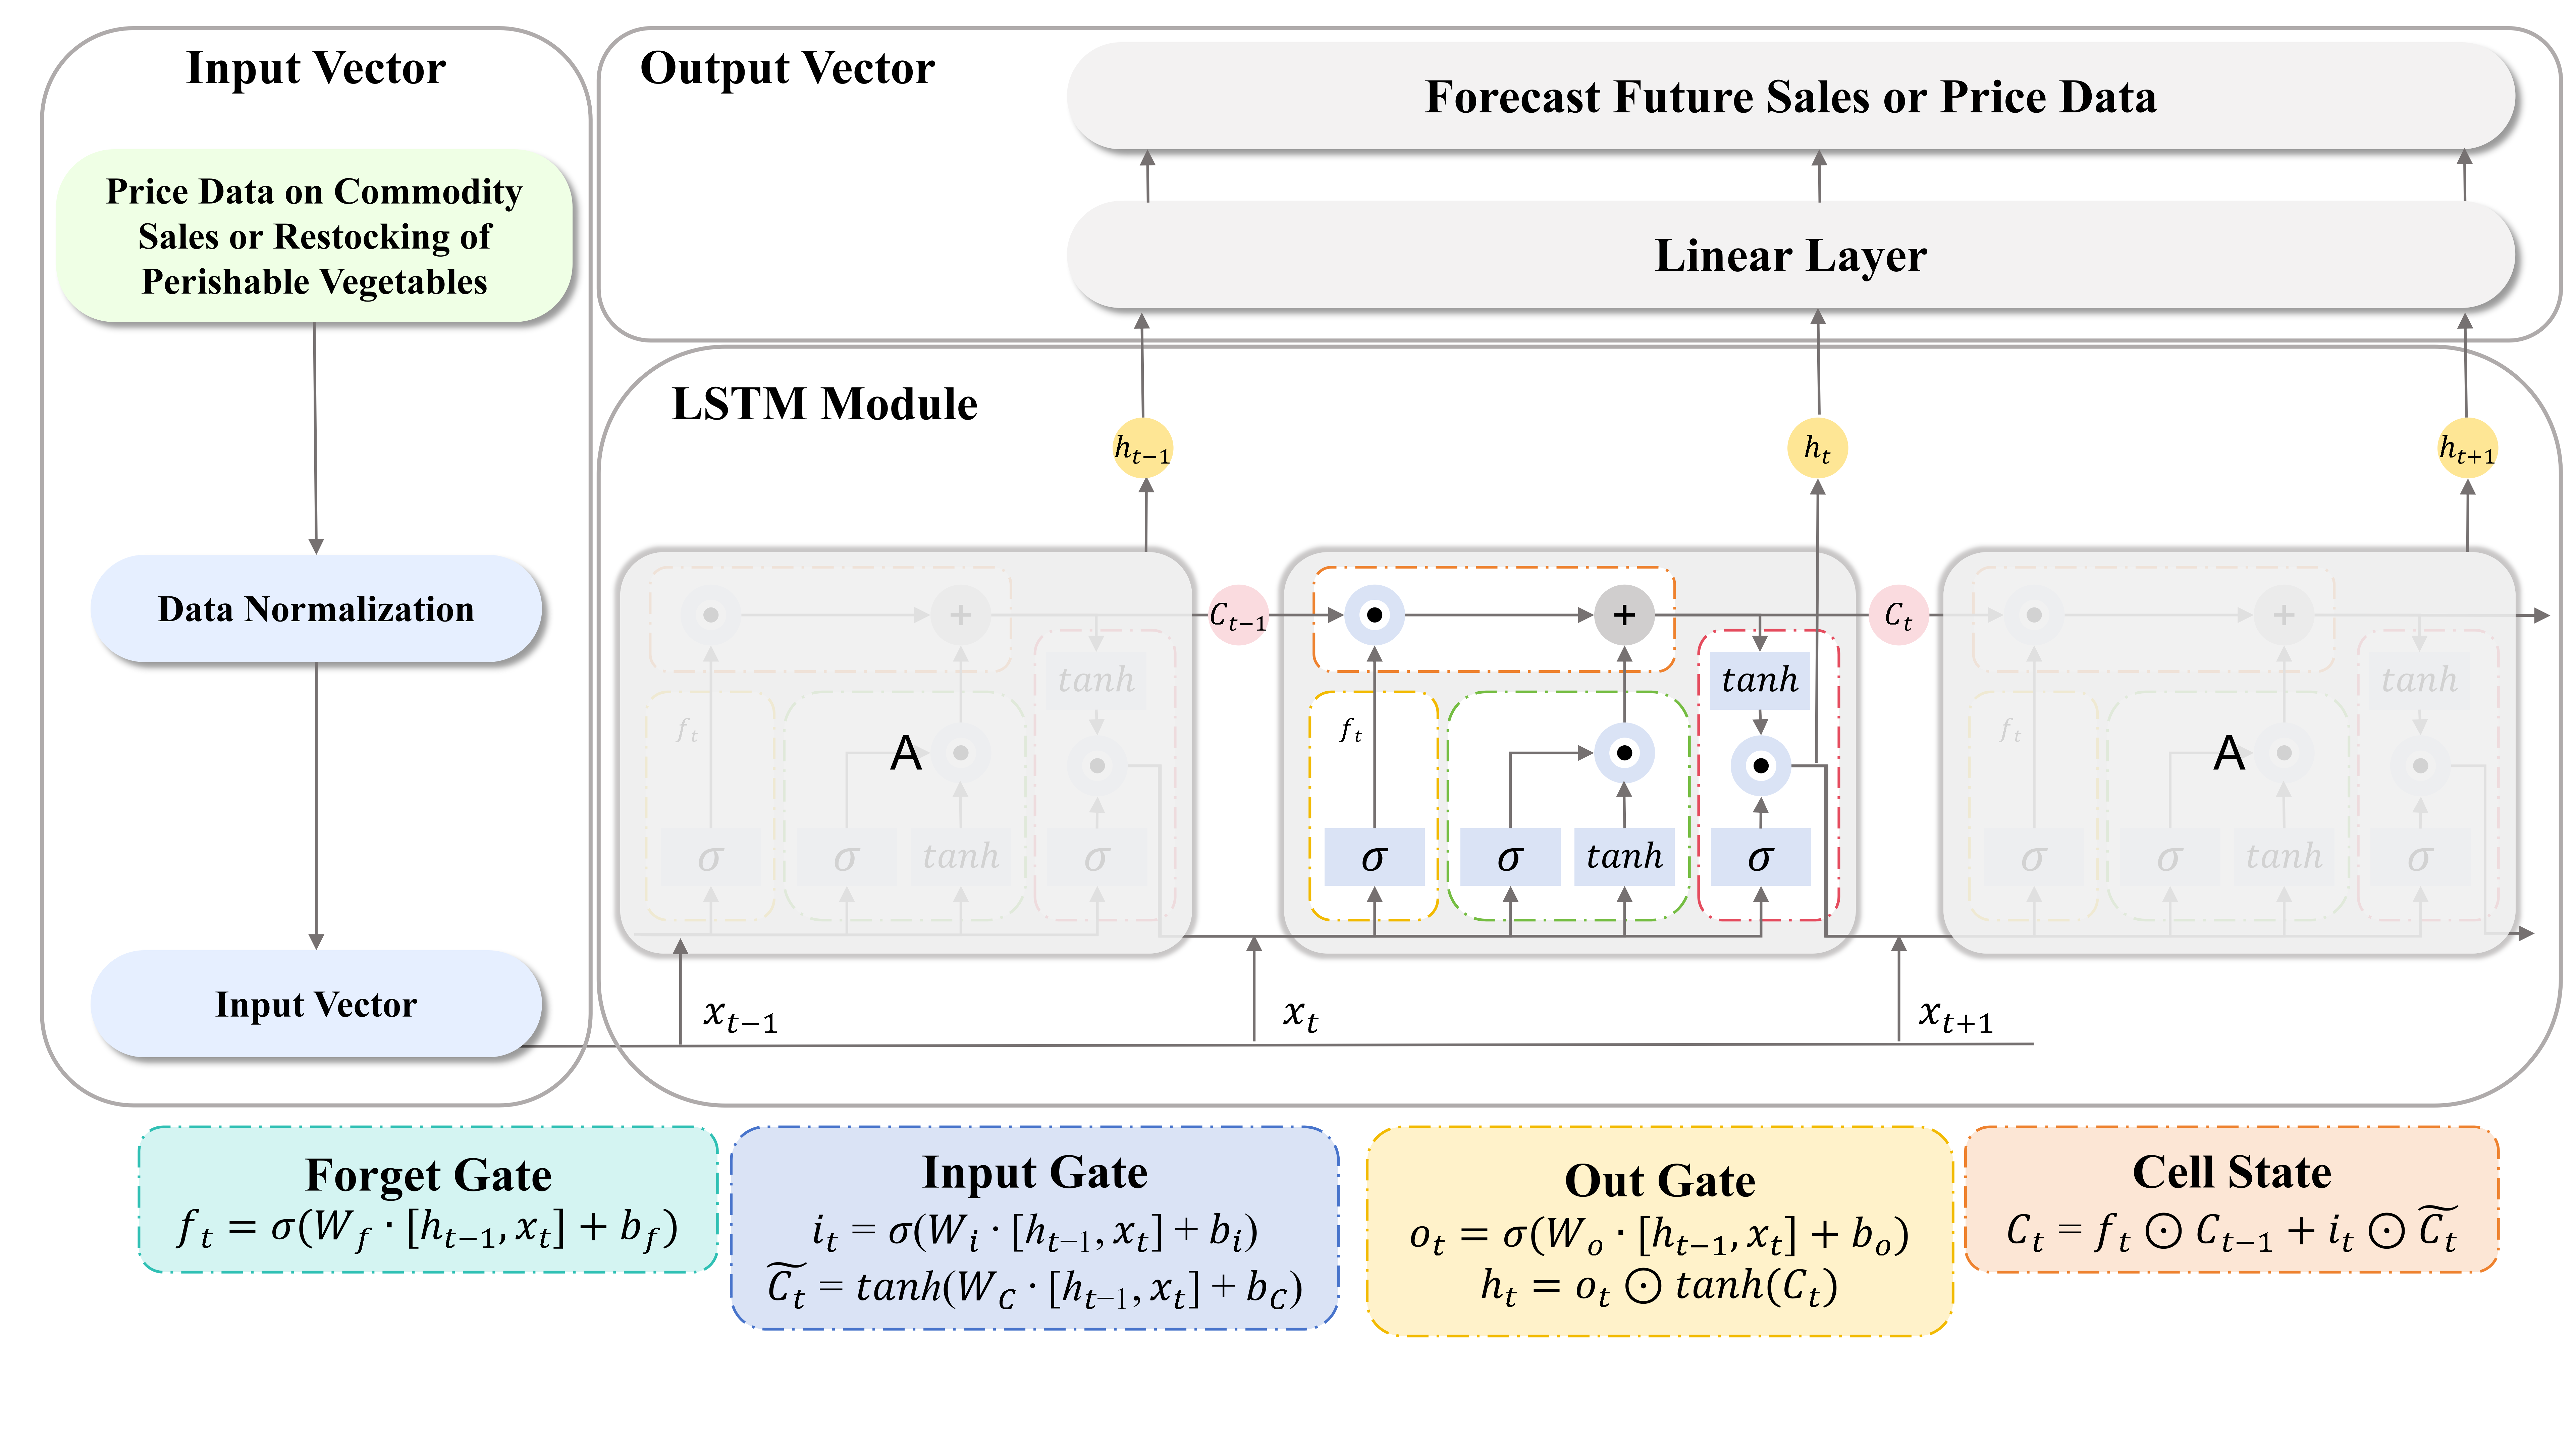
\includegraphics[width=0.9\textwidth]{图片2.png}
        \caption{LSTM模型架构}
        \label{fig:fig2}
\end{figure}

\subsubsection{KAN-LSTM模型}
\label{subsubsec:kan_lstm_model}

柯尔莫哥洛夫-阿诺德网络(KAN)是基于柯尔莫哥洛夫-阿诺德表示定理的神经网络架构。其核心思想是将任意多元连续函数表示为单变量函数的叠加与复合\citep{Ismailov2008,Genet2024}。该网络架构的数学推导详见附录A。为融合KAN与LSTM优势,构建KAN-LSTM模型如下:

\paragraph{KAN层输入变换}  
KAN层通过单变量映射$\phi_{q,p}$转换输入$x_t$:  
\begin{equation}
\hat{x}_{t,q} = \sum_{p=1}^{n} \phi_{q,p} \left( W_{x,p} x_{t,p} + b_{x,p} \right)
\end{equation}

\paragraph{RKAN状态更新}  
递归柯尔莫哥洛夫-阿诺德网络(RKAN)通过递归应用KAN层变换管理时间序列依赖关系:  
\begin{equation}
h_t = \sum_{q=1}^{2n+1} \Phi_q(\tilde{x}_{t,q})
\end{equation}
其中$\Phi_q$为KAN层学习的单变量映射函数。

\paragraph{LSTM门控机制融合}  
为增强模型捕捉长短期依赖能力,将LSTM门控机制融入RKAN隐藏状态更新过程:  
\begin{align}
f_t &= \sigma(W_{f,h}h_{t-1} + W_{f,x}x_t + b_f) \\
i_t &= \sigma(W_{i,h}h_{t-1} + W_{i,x}x_t + b_i) \\
\tilde{c}_t &= \tanh(W_{c,h}h_{t-1} + W_{c,x}x_t + b_c) \\
c_t &= f_t \odot c_{t-1} + i_t \odot \tilde{c}_t \\
o_t &= \sigma(W_{o,h}h_{t-1} + W_{o,x}x_t + b_o) \\
h_t &= o_t \odot \tanh(c_t)
\end{align}
KAN-LSTM最终架构如图\ref{fig:fig3}所示:

\begin{figure}[H]
        \centering
        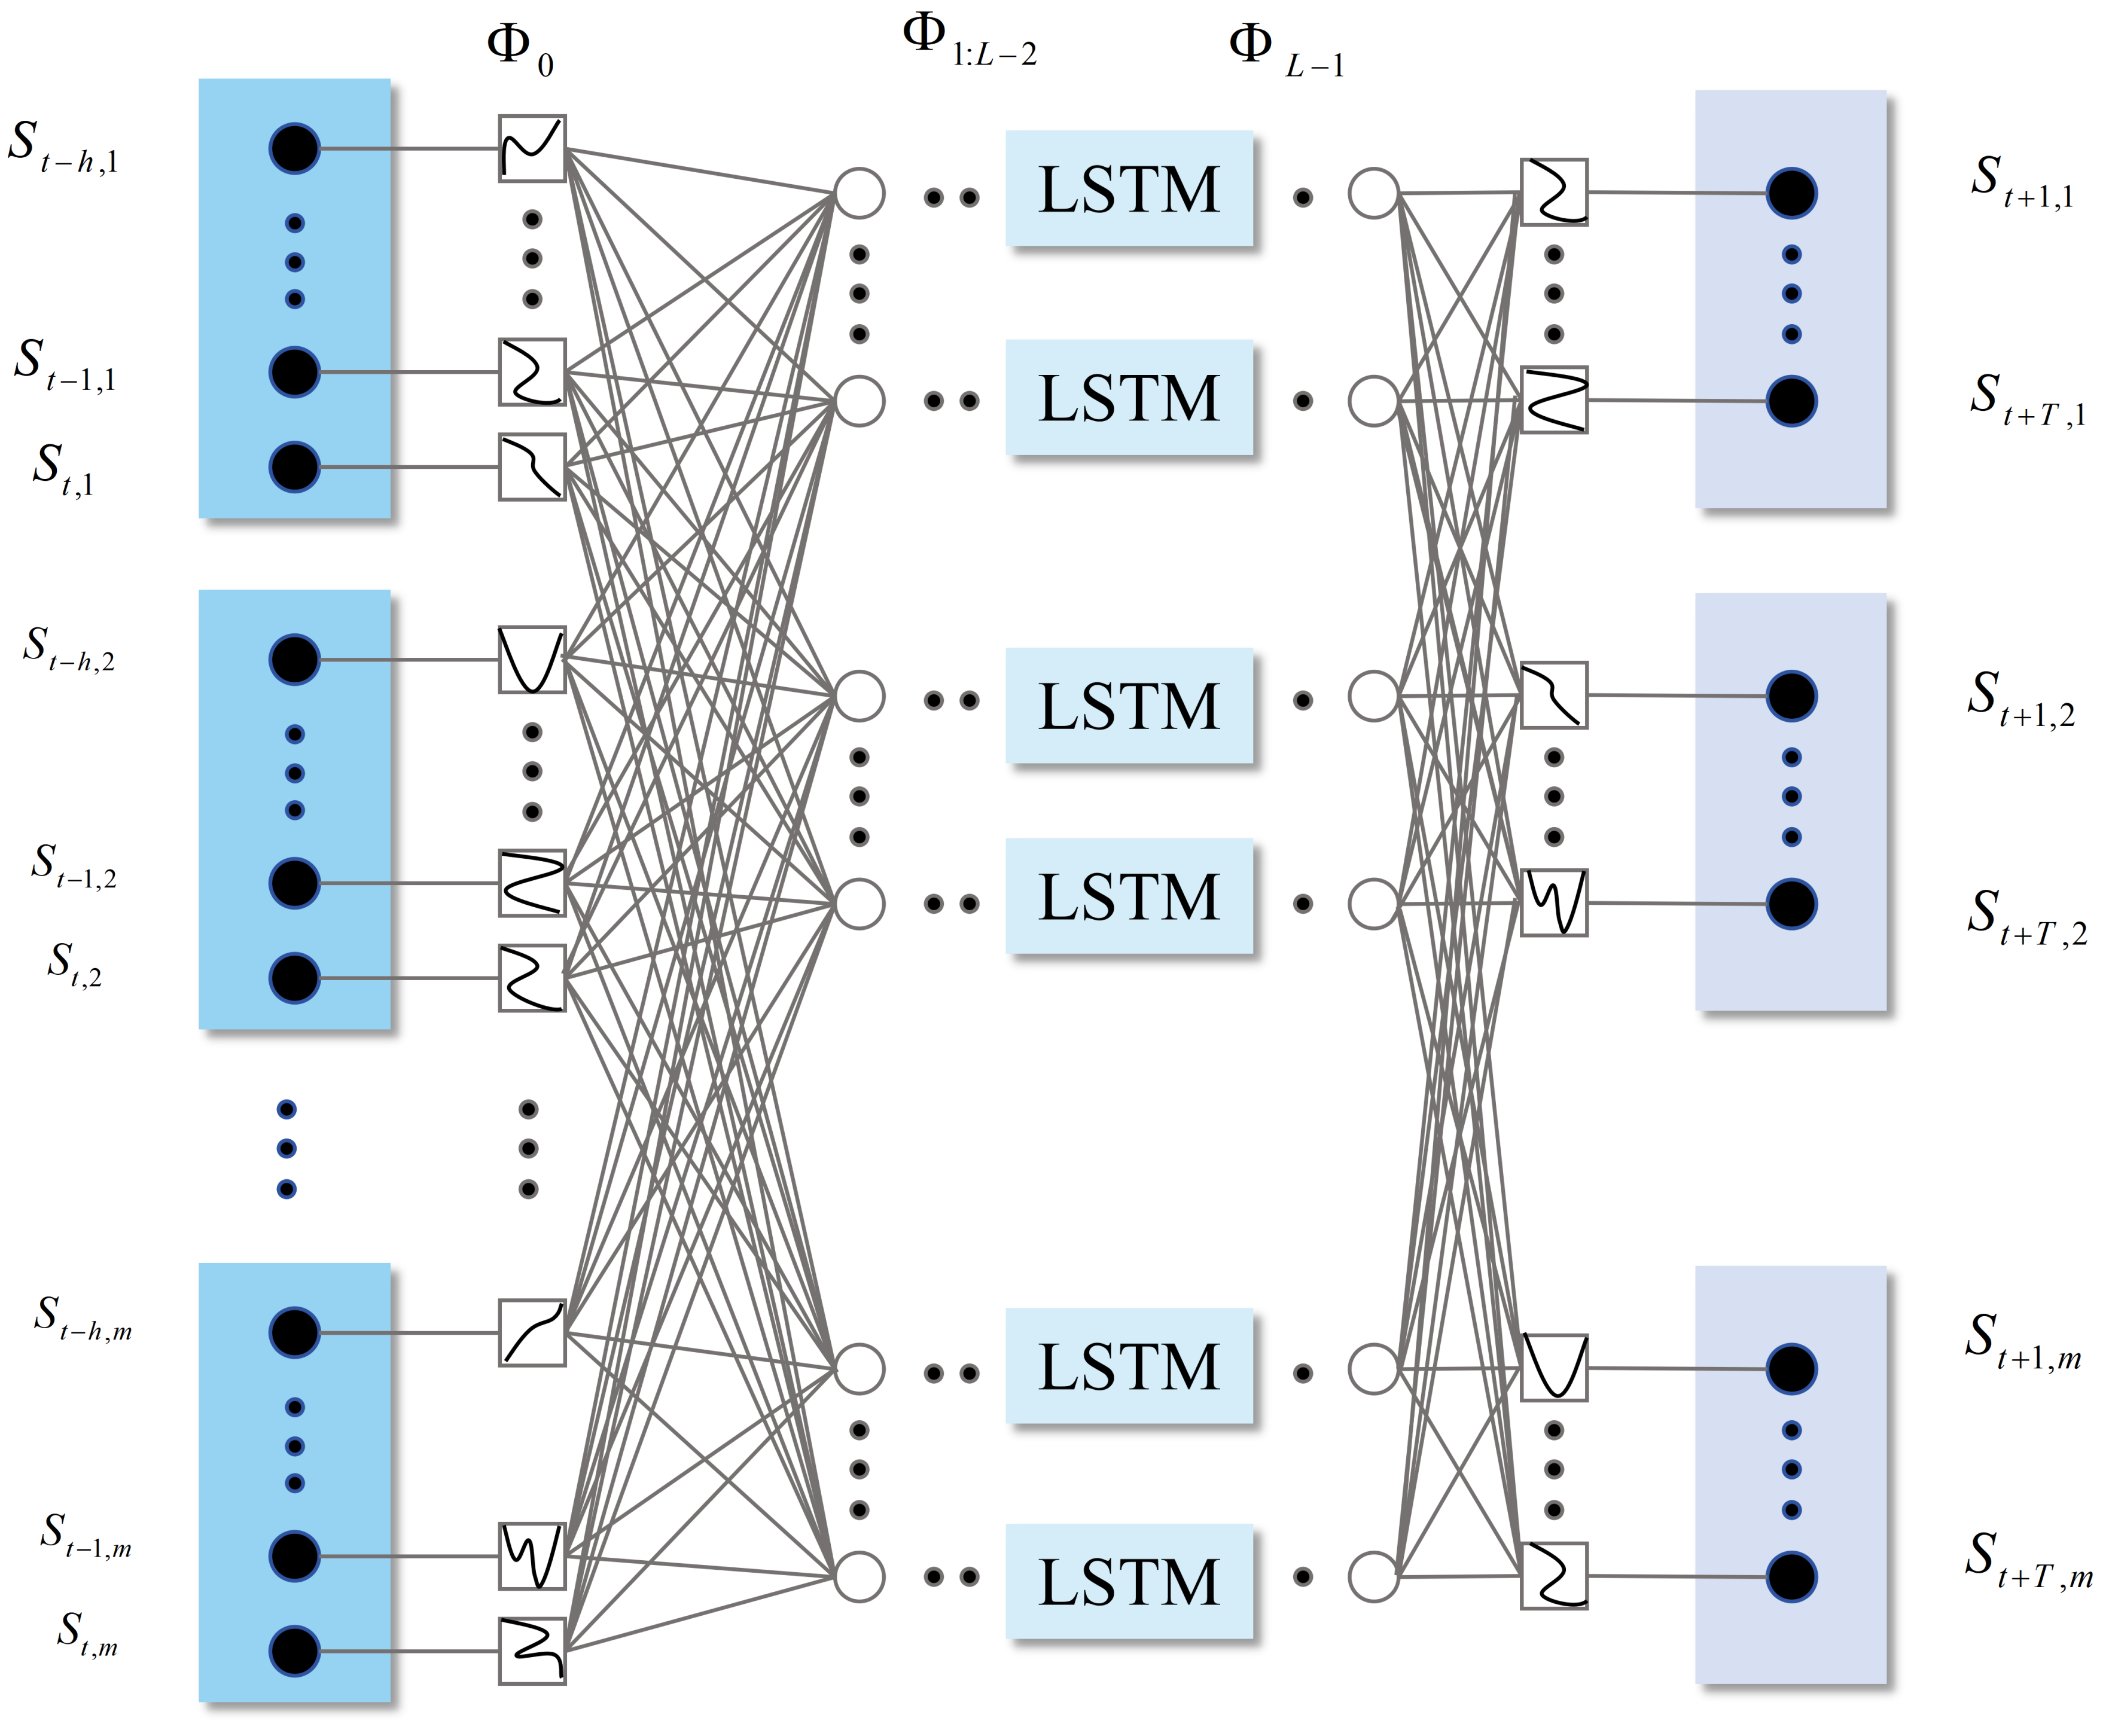
\includegraphics[width=0.9\textwidth]{图片3.png}
        \caption{KAN-LSTM模型架构}
        \label{fig:fig3}
\end{figure}

\subsubsection{模型评价指标}
\label{subsubsec:model_evaluation_metrics}
为全面评估预测值与实际观测值的偏离程度,本研究选用三种常用评价指标:决定系数($R^2$)、均方根误差(RMSE)和平均绝对百分比误差(MAPE)。其定义如下:

\begin{equation}
R^2 = 1 - \frac{\sum_{i=1}^{n} (y_i - \hat{y}_i)^2}{\sum_{i=1}^{n} (y_i - \bar{y})^2},
\end{equation}

\begin{equation}
RMSE = \sqrt{\frac{1}{n} \sum_{i=1}^{n} (y_i - \hat{y}_i)^2},
\end{equation}

\begin{equation}
MAPE = \frac{1}{n} \sum_{i=1}^{n} \left| \frac{y_i - \hat{y}_i}{y_i} \right| \times 100,
\end{equation}
其中$y_i$为实际观测值,$\hat{y}_i$为模型预测值,$\bar{y}$为实际值样本均值,$n$为样本量。上述指标将用于评估模型在训练集与测试集上的性能,验证所提方法的准确性与可靠性。
\subsection{优化方法}
\label{subsec:optimization_method}
订货策略优化需综合考虑定价、需求预测与库存管理,实现利润最大化目标。本研究通过三部分构建优化模型:成本加成定价模型、需求回归模型及非线性规划模型构建。

\subsubsection{成本加成定价模型}
\label{subsubsec:cost_plus_pricing}
成本加成定价是订货策略的基础,其核心通过在进货成本上加成确定产品销售价格。定价公式为:
\begin{equation}
p_i = c_i  (1 + m_i),
\end{equation}
其中$p_i$表示产品销售价格,$c_i$表示产品进货成本,$m_i$表示产品加价率。

合理的加价率$m_i$是后续规划模型中的关键决策变量。确定最优加价率需结合需求回归模型与规划目标进行综合优化。

\subsubsection{需求回归模型}
\label{subsubsec:demand_regression_model}
产品需求$D_i$不仅取决于自身价格$p_i$,更受相关产品价格$p_j$与销量$D_j$的非线性影响。为捕捉价格弹性与交叉弹性效应,基于弹性理论构建多元需求回归模型,其对数形式为:

\begin{equation}
\ln(D_i) = \alpha - \beta \ln(p_i) + \sum_j \gamma_j \ln(p_j) + \sum_j \delta_j \ln(D_j),
\end{equation}

式中$\alpha$为规模参数,$\beta$为自身价格弹性,$\gamma_j$、$\delta_j$分别为交叉价格弹性与交叉销量弹性系数。

结合成本加成定价公式,需求函数转换为:

\begin{equation}
D_i = e^{\alpha} [c_i(1 + m_i)]^{-\beta} \prod_j p_j^{\gamma_j} \prod_j D_j^{\delta_j}.
\end{equation}

通过估计参数$\alpha$、$\beta$、$\gamma_j$和$\delta_j$,可量化自身价格效应、交叉价格效应及交叉销量关系对需求的影响,为定价与订货决策提供依据。

\subsubsection{非线性规划模型构建}
\label{subsubsec:nonlinear_programming_model}
基于成本加成定价与需求回归模型,以进货量$Q_i$和加价率$m_i$为决策变量,构建考虑库存成本的利润最大化非线性规划模型:

\paragraph{目标函数}
店铺总利润由销售利润与库存成本构成:
\begin{equation}
\max_{Q, m} \text{Profit} = \sum_i [(p_i - c_i)  D_i - h_i  (Q_i - D_i)],
\end{equation}
其中$(p_i - c_i)  D_i$为产品销售利润,$h_i  (Q_i - D_i)$为库存持有成本,$h_i$为第$i$种产品损耗率,$Q_i$为产品进货量\footnote{在本文使用的数据集中,农贸市场并未形成日度记录损耗率的制度,因此本文中的损耗率均为不随时间变化的固定值,详细见https://github.com/Zhanli-Li/Digital-Agricultural-Economics}。

\paragraph{约束条件1:需求满足约束}
订货量至少需满足需求,确保库存非负:
\begin{equation}
Q_i \geq e^{\alpha_i} \cdot \left[ c_i \cdot (1 + m_i) \right]^{-\beta_i} \prod_j p_j^{\gamma_{ij}} \prod_j D_j^{\delta_{ij}}, \quad \forall i.
\end{equation}

\paragraph{约束条件2:加价率范围约束}
加价率需处于合理区间:
\begin{equation}
m_{\text{min}} \leq m_i \leq m_{\text{max}}, \quad \forall i.
\end{equation}

\paragraph{优化模型数学形式}
整合目标函数与约束条件,得完整优化模型:

\textbf{目标函数:}
\begin{equation}
\max_{Q, m} \quad \text{Profit} = \sum_i \left[ (p_i - c_i) \cdot D_i - h_i \cdot (Q_i - D_i) \right].
\end{equation}

\textbf{约束条件:}
\begin{equation}
\begin{cases}
Q_i &\geq e^{\alpha_i} \cdot \left[ c_i \cdot (1 + m_i) \right]^{-\beta_i} \prod_j p_j^{\gamma_{ij}} \prod_j D_j^{\delta_{ij}}, \quad \forall i \\
m_{\min} &\leq m_i \leq m_{\max}, \quad \forall i \\
D_i &= e^{\alpha_i} \cdot \left[ c_i \cdot (1 + m_i) \right]^{-\beta_i} \prod_j p_j^{\gamma_{ij}} \prod_j D_j^{\delta_{ij}} \\
p_i &= c_i \cdot (1 + m_i), \quad \forall i
\end{cases}
\end{equation}
\section{结果分析}
\label{sec:results}
本节展示KAN-LSTM模型预测性能与订货策略优化的实证结果。第\ref{subsec:prediction_results}节报告预测模型结果,第\ref{subsec:ordering_strategy}节阐述订货策略优化结果。

\subsection{KAN-LSTM模型预测结果}
\label{subsec:prediction_results}
本研究基于花菜类等六类生鲜蔬菜历史销售数据构建KAN-LSTM模型。模型训练超参数设置如表\ref{tab:hyperparameters}所示,数据集按7:3比例划分为训练集与测试集。

\begin{table}[H]
\centering
\caption{超参数配置}
\label{tab:hyperparameters}
\begin{tabular}{lcc}
\toprule
\textbf{超参数} & \textbf{取值} \\
\midrule
隐藏层数量 & 2 \\
单隐藏层单元数 & 6 \\
全连接层神经元数 & 7 \\
激活函数 & ReLU \\
优化器 & Adam \\
学习率 & 0.001 - 0.005 \\
损失函数 & 均方误差(MSE) \\
训练轮次 & 400 \\
\bottomrule
\end{tabular}
\end{table}

基于上述参数配置进行模型训练,记录损失函数值变化过程。通过损失函数曲线收敛趋势分析,证实KAN-LSTM模型在各类数据集上均达到稳定收敛状态。

\begin{figure}[H]
    \centering
    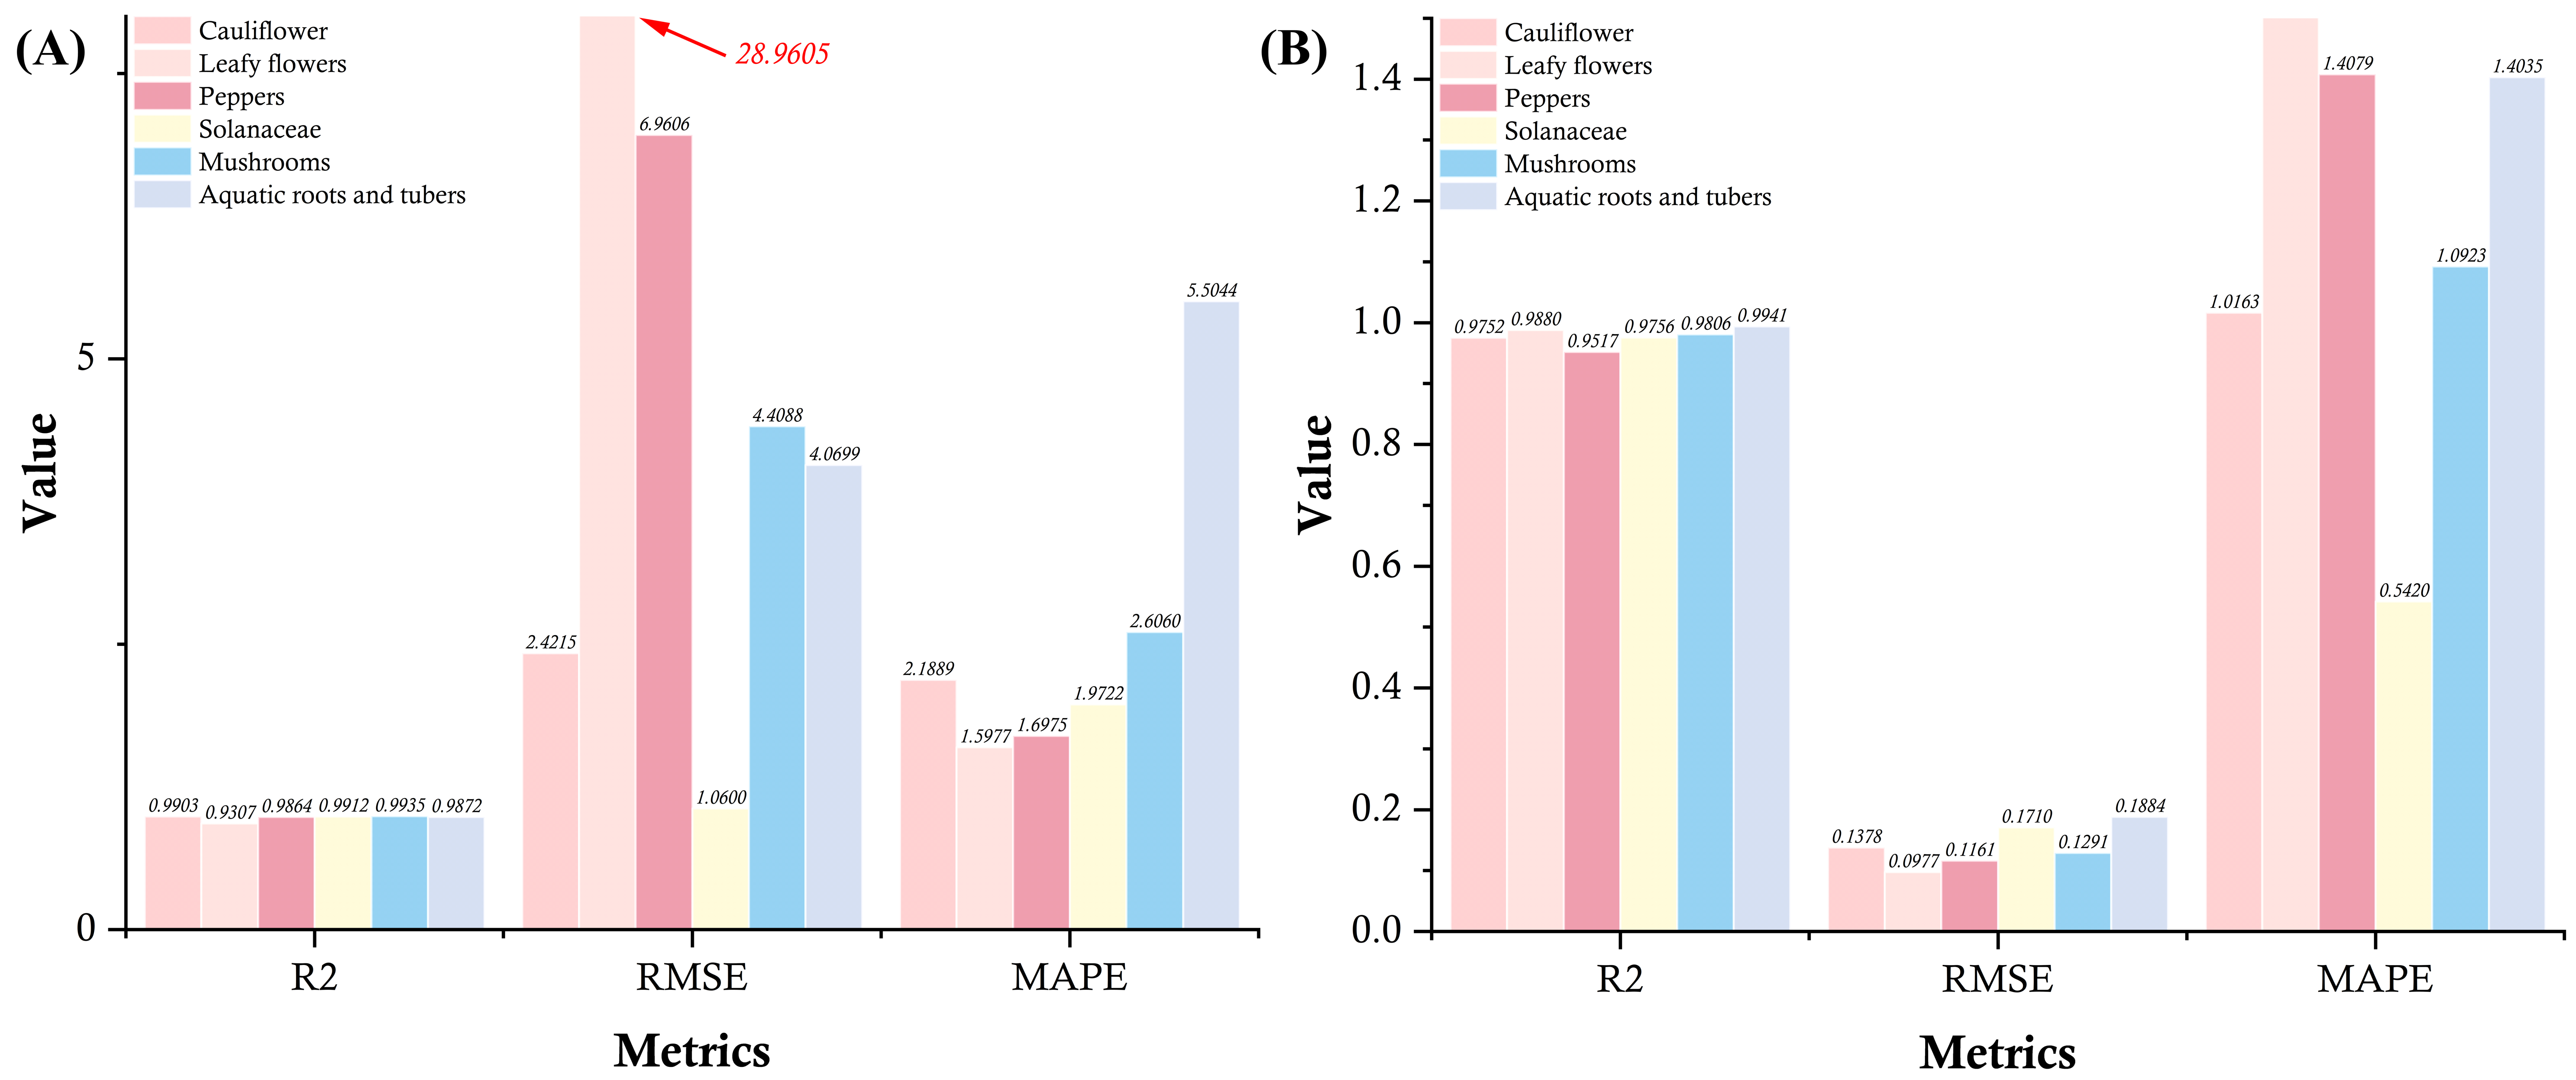
\includegraphics[width=1\textwidth]{图片4.png}
    \caption{预测性能评估。(A)销量数据预测效果 (B)进货价格预测效果}
    \label{fig:fig4}
\end{figure}

图\ref{fig:fig4}(A)(B)显示:KAN-LSTM模型在销量与进货价格预测中均表现优异。$R^2$值表明花菜类、叶菜类等六类产品的预测值与实际值高度吻合,模型整体拟合优度优越。RMSE与MAPE指标在多数品类处于较低水平,进一步验证模型捕捉复杂时间序列模式及非线性关系的能力。但叶菜类等品类RMSE值偏高,反映其数据波动性或市场不确定性较强。综合而言,KAN-LSTM在农产品销量与价格预测中展现出色精度。

\subsection{订货策略优化结果}
\label{subsec:ordering_strategy}

\subsubsection{需求回归模型参数估计}
\label{subsubsec:demand_regression_results}
采用多元逐步回归法求解需求模型,通过回归系数及其显著性水平(P值)识别影响需求变动的关键解释变量。最终回归模型参数估计及显著性结果见图\ref{fig:fig5}与表\ref{tab:param_estimates}。

如图\ref{fig:fig5}所示,六类蔬菜需求回归模型拟合良好:调整后$R^2$值介于0.545-0.839,F统计量均显著(p<0.05),表明模型整体显著且能有效解释需求变动。基于预测结果构建非线性规划模型如下:

\begin{equation}
\max_{Q,m} \quad \text{Profit} = \sum_i \left[ (p_i - c_i) \cdot D_i - h_i \cdot (Q_i - D_i) \right]
\end{equation}
\text{约束条件:}
\begin{equation}
\begin{cases}
Q_i \geq e^{\alpha_i} \cdot \left[ c_i \cdot (1 + m_i) \right]^{-\beta_i} \prod_j p_j^{\gamma_{ij}} \prod_j D_j^{\delta_{ij}}, & \forall i \\
m_{\min} \leq m_i \leq m_{\max}, & \forall i \\
D_C = e^{2.1886} \cdot p_C^{-0.9857} \cdot p_S^{0.5908} \cdot D_M^{0.4195} \cdot D_L^{0.4908}, & \text{花菜类需求} \\
D_L = e^{3.1204} \cdot p_L^{-0.6574} \cdot p_C^{0.3061} \cdot D_P^{0.2717} \cdot D_M^{0.3482} \cdot D_C^{0.2072}, & \text{叶菜类需求} \\
D_P = e^{3.2775} \cdot p_P^{-0.5992} \cdot p_M^{0.2702} \cdot D_M^{0.5095} \cdot D_S^{0.1585} \cdot D_C^{0.1067}, & \text{椒类需求} \\
D_S = e^{-2.9685} \cdot p_C^{0.5727} \cdot D_P^{0.6752} \cdot D_M^{0.4111}, & \text{茄果类需求} \\
D_M = e^{-0.4126} \cdot p_M^{-0.3457} \cdot p_P^{0.5006} \cdot D_P^{0.7163} \cdot D_L^{0.3453}, & \text{食用菌类需求} \\
D_A = e^{-0.9428} \cdot p_L^{-1.5807} \cdot p_S^{0.7967} \cdot D_P^{1.0462}, & \text{水生块根类需求} \\
p_i = c_i \cdot (1 + m_i), & \forall i
\end{cases}
\end{equation}

其中$D_C$、$D_L$、$D_P$、$D_S$、$D_M$、$D_A$分别表示花菜类、叶菜类、椒类、茄果类、食用菌类及水生块根类销量;$P_C$、$P_L$、$P_P$、$P_S$、$P_M$、$P_A$表示相应品类批发价格(含加价率)。

\begin{figure}[H]
    \centering
    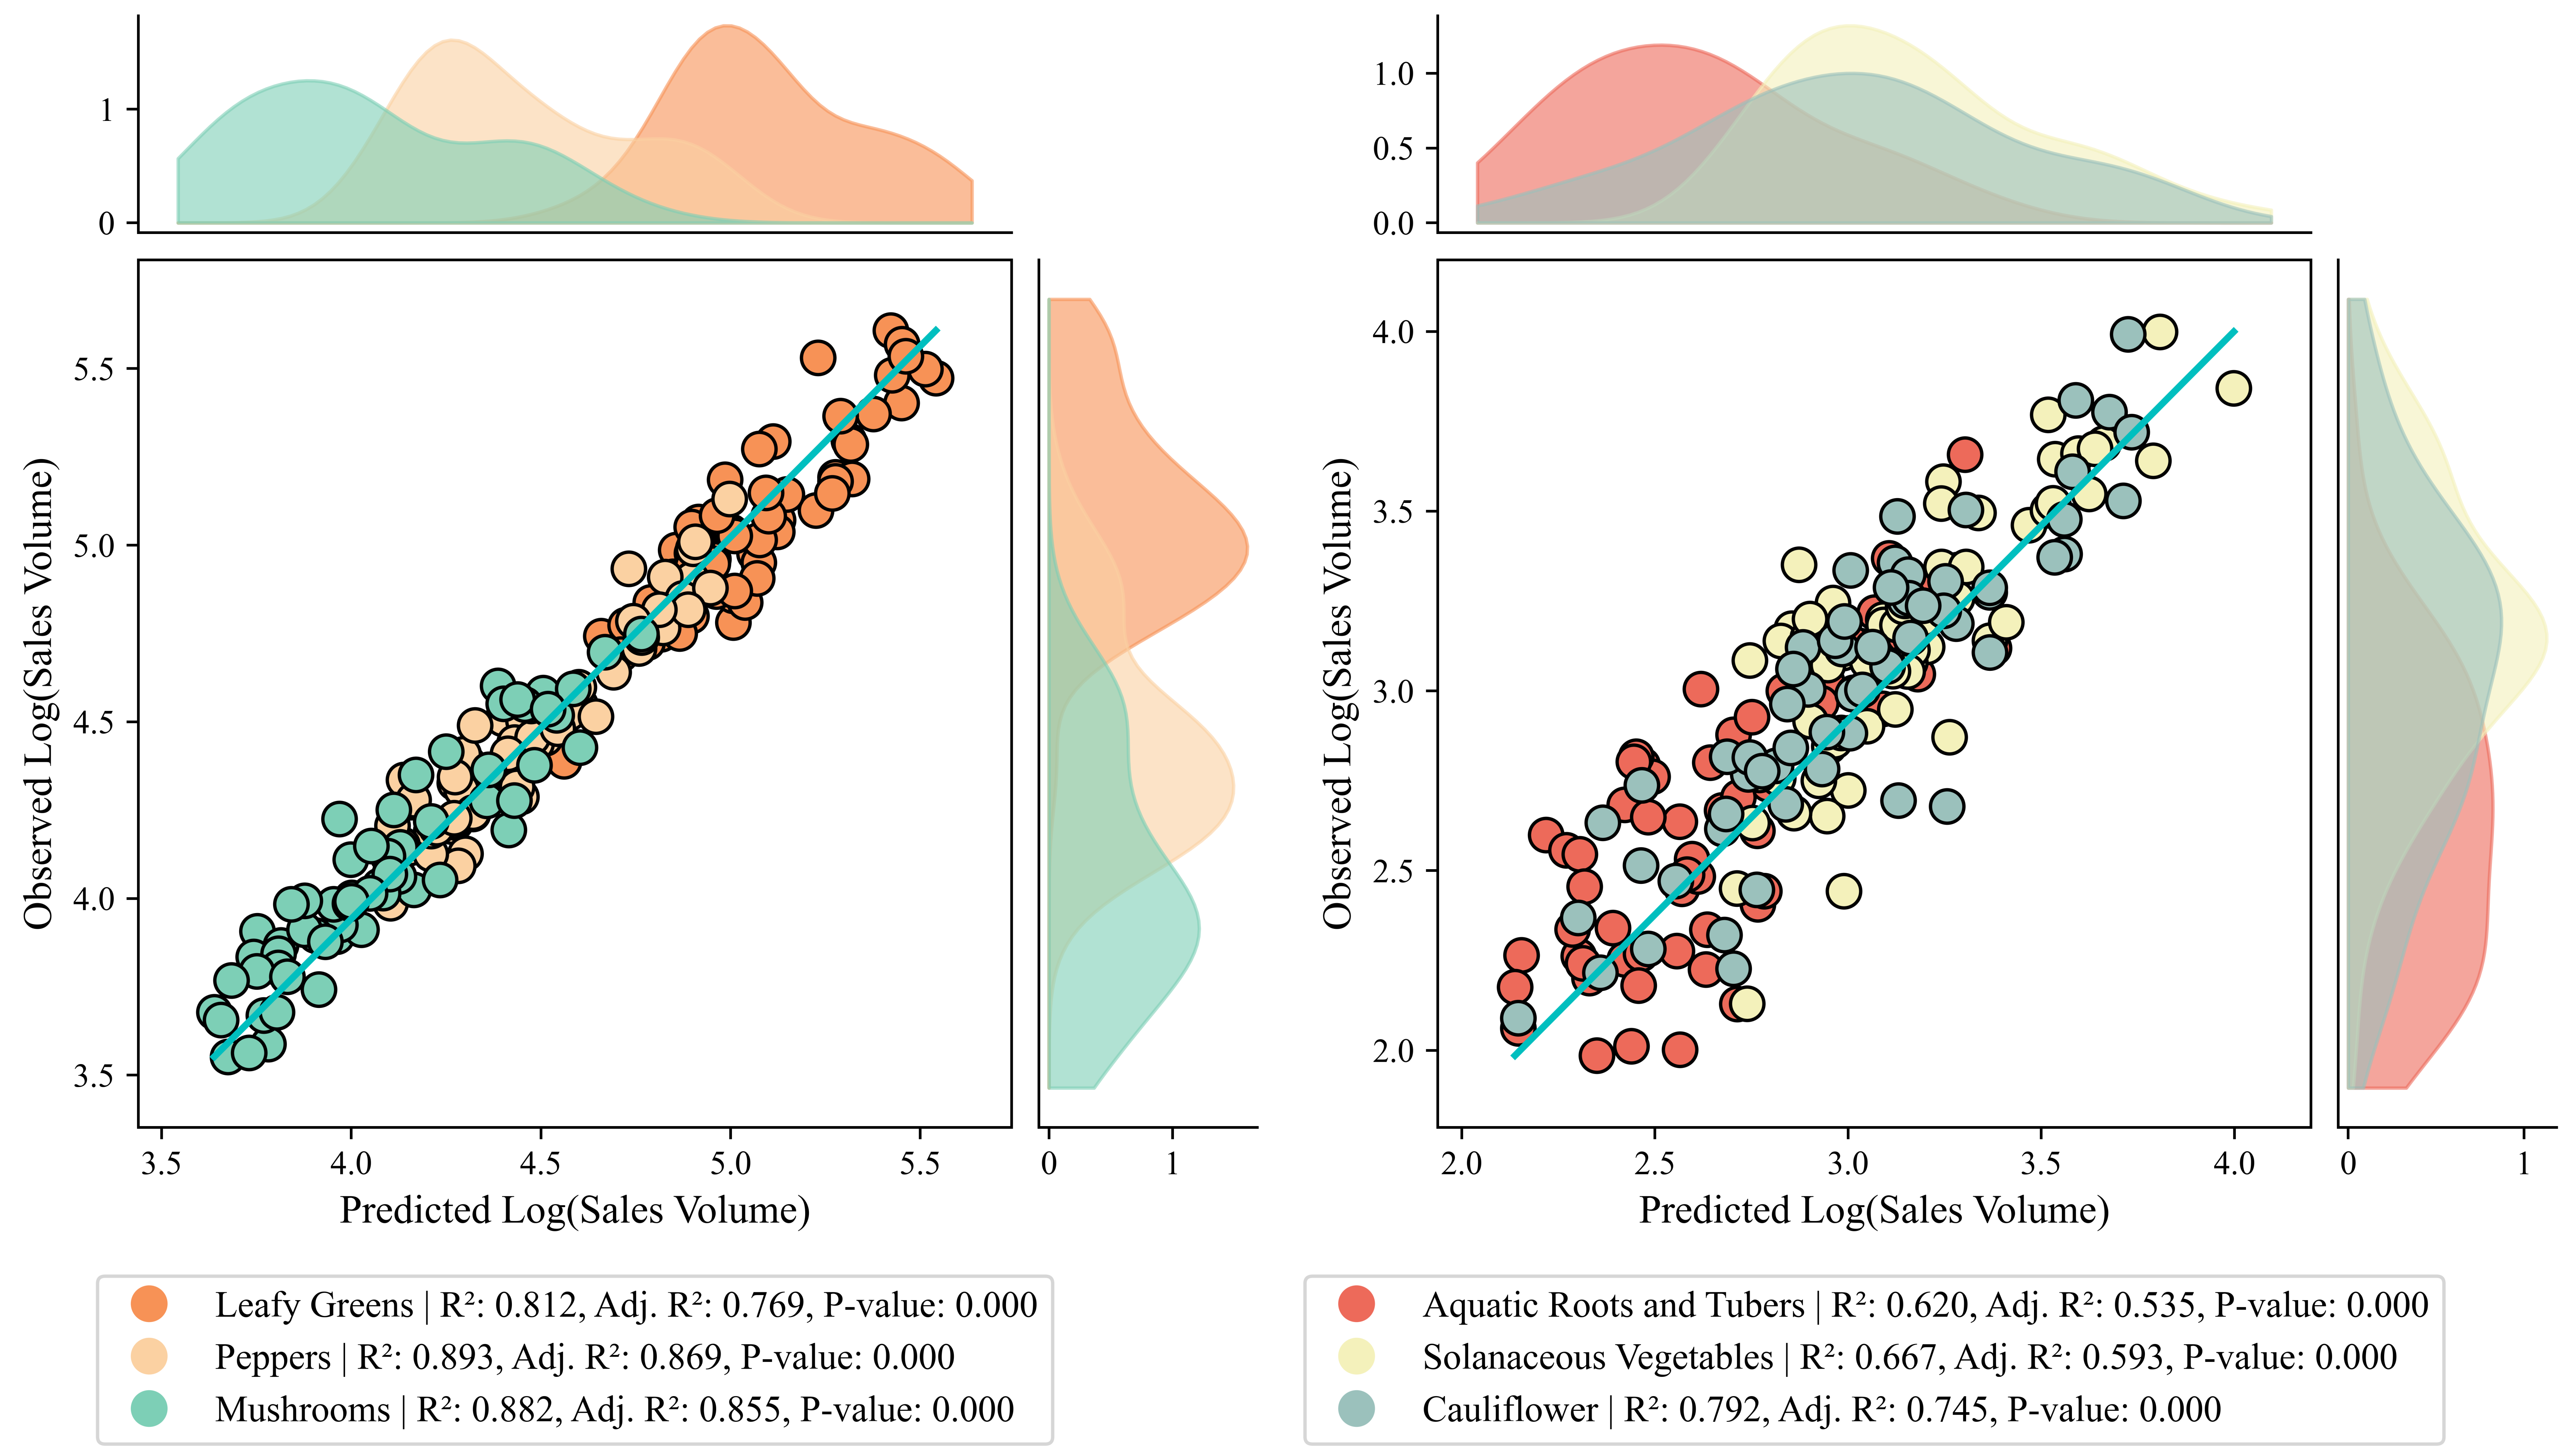
\includegraphics[width=1\textwidth]{图片5.png}
    \caption{需求回归模型估计结果}
    \label{fig:fig5}
\end{figure}

\begin{table}[H]
    \centering
    \caption{参数估计与显著性检验结果}
    \begin{tabular}{cccccc}
    \toprule
    \textbf{模型I} & \textbf{模型II} & \textbf{模型III} & \textbf{模型IV} & \textbf{模型V} & \textbf{模型VI} \\
    \midrule
    \textbf{常数项} & \textbf{常数项} & \textbf{常数项} & \textbf{常数项} & \textbf{常数项} & \textbf{常数项} \\
    (2.1886**) & (3.1204***) & (3.2775***) & (-2.6385***) & (-0.4126) & (-0.9428) \\
    $p_C$ & $p_L$ & $p_P$ & $p_C$ & $p_M$ & $p_L$ \\
    (-0.9857***) & (-0.6574***) & (-0.5992***) & (0.5727***) & (-0.3457***) & (-1.5807***) \\
    $p_S$ & $p_C$ & $p_M$ & $p_P$ & $p_P$ & $p_S$ \\
    (0.5908**) & (0.3061**) & (0.2702**) & (0.6752***) & (0.5006***) & (0.7967**) \\
    $D_M$ & $D_P$ & $D_M$ & $D_M$ & $D_P$ & $D_P$ \\
    (0.4195***) & (0.2717**) & (0.5095***) & (0.4111**) & (0.7163***) & (1.0462***) \\
    $D_L$ & $D_M$ & $D_S$ & \ & $D_L$ & \ \\
    (0.4908***) & (0.3482***) & (0.1585***) & \ & (0.3453***) & \ \\
    \ & $D_C$ & $D_C$ & \ & \ & \ \\
    \ & (0.2072***) & (0.1067**) & \ & \ & \ \\
    \bottomrule
    \end{tabular}
    \label{tab:param_estimates}
\end{table}
\begin{tablenotes}
\footnotesize
\item 注:模型I-VI分别对应$D_C$、$D_L$、$D_P$、$D_S$、$D_M$、$D_A$,括号内为系数估计值与显著性水平。***、**、*分别表示1\%、5\%、10\%显著性水平。
\end{tablenotes}

\subsubsection{未来15日订货决策求解}
\label{subsubsec:ordering_decision_15_days}

\textbf{定理1:} 在特定条件下,本文提出的批发市场供应链管理与订货策略优化问题为凸优化问题。具体而言,若各类产品需求函数$D_i$满足:
\begin{equation}
D_i = e^{\alpha_i} \left[ c_i (1 + m_i) \right]^{-\beta_i} \prod_j p_j^{\gamma_{ij}} \prod_j D_j^{\delta_{ij}},
\end{equation}
且$\beta_i \leq -1$或$\beta_i \geq 0$,则目标函数与约束条件定义的可行域为凸集。此时优化问题具有凸性,可采用凸优化算法获取全局最优解。定理证明见附录B。

基于表\ref{tab:param_estimates}需求函数及定理1分析:模型I($\beta_i$=-0.9857)和模型II($\beta_i$=-0.6574)满足凹函数条件;模型III($\beta_i$=-0.5992)与模型IV($\beta_i$=-0.5727)仍保持非凸性;模型V($\beta_i$=-0.3457)亦为非凸;模型VI因逐步回归剔除价格弹性变量而成为凸函数。整体而言,订货决策模型呈凹性结构。

需求函数凸凹性差异表明优化问题可能存在非凸性,增加全局最优解搜索难度。因此采用粒子群优化(PSO)、遗传算法(GA)等全局搜索算法提升解的可靠性与有效性。

基于需求预测模型与目标函数,本研究采用模拟退火算法\citep{Tavares2011}求解未来15日订货量与加价率。优化过程引入约束条件保证解可行性,最终实现总利润最大化(图\ref{fig:fig6})。

\begin{figure}[H]
    \centering
    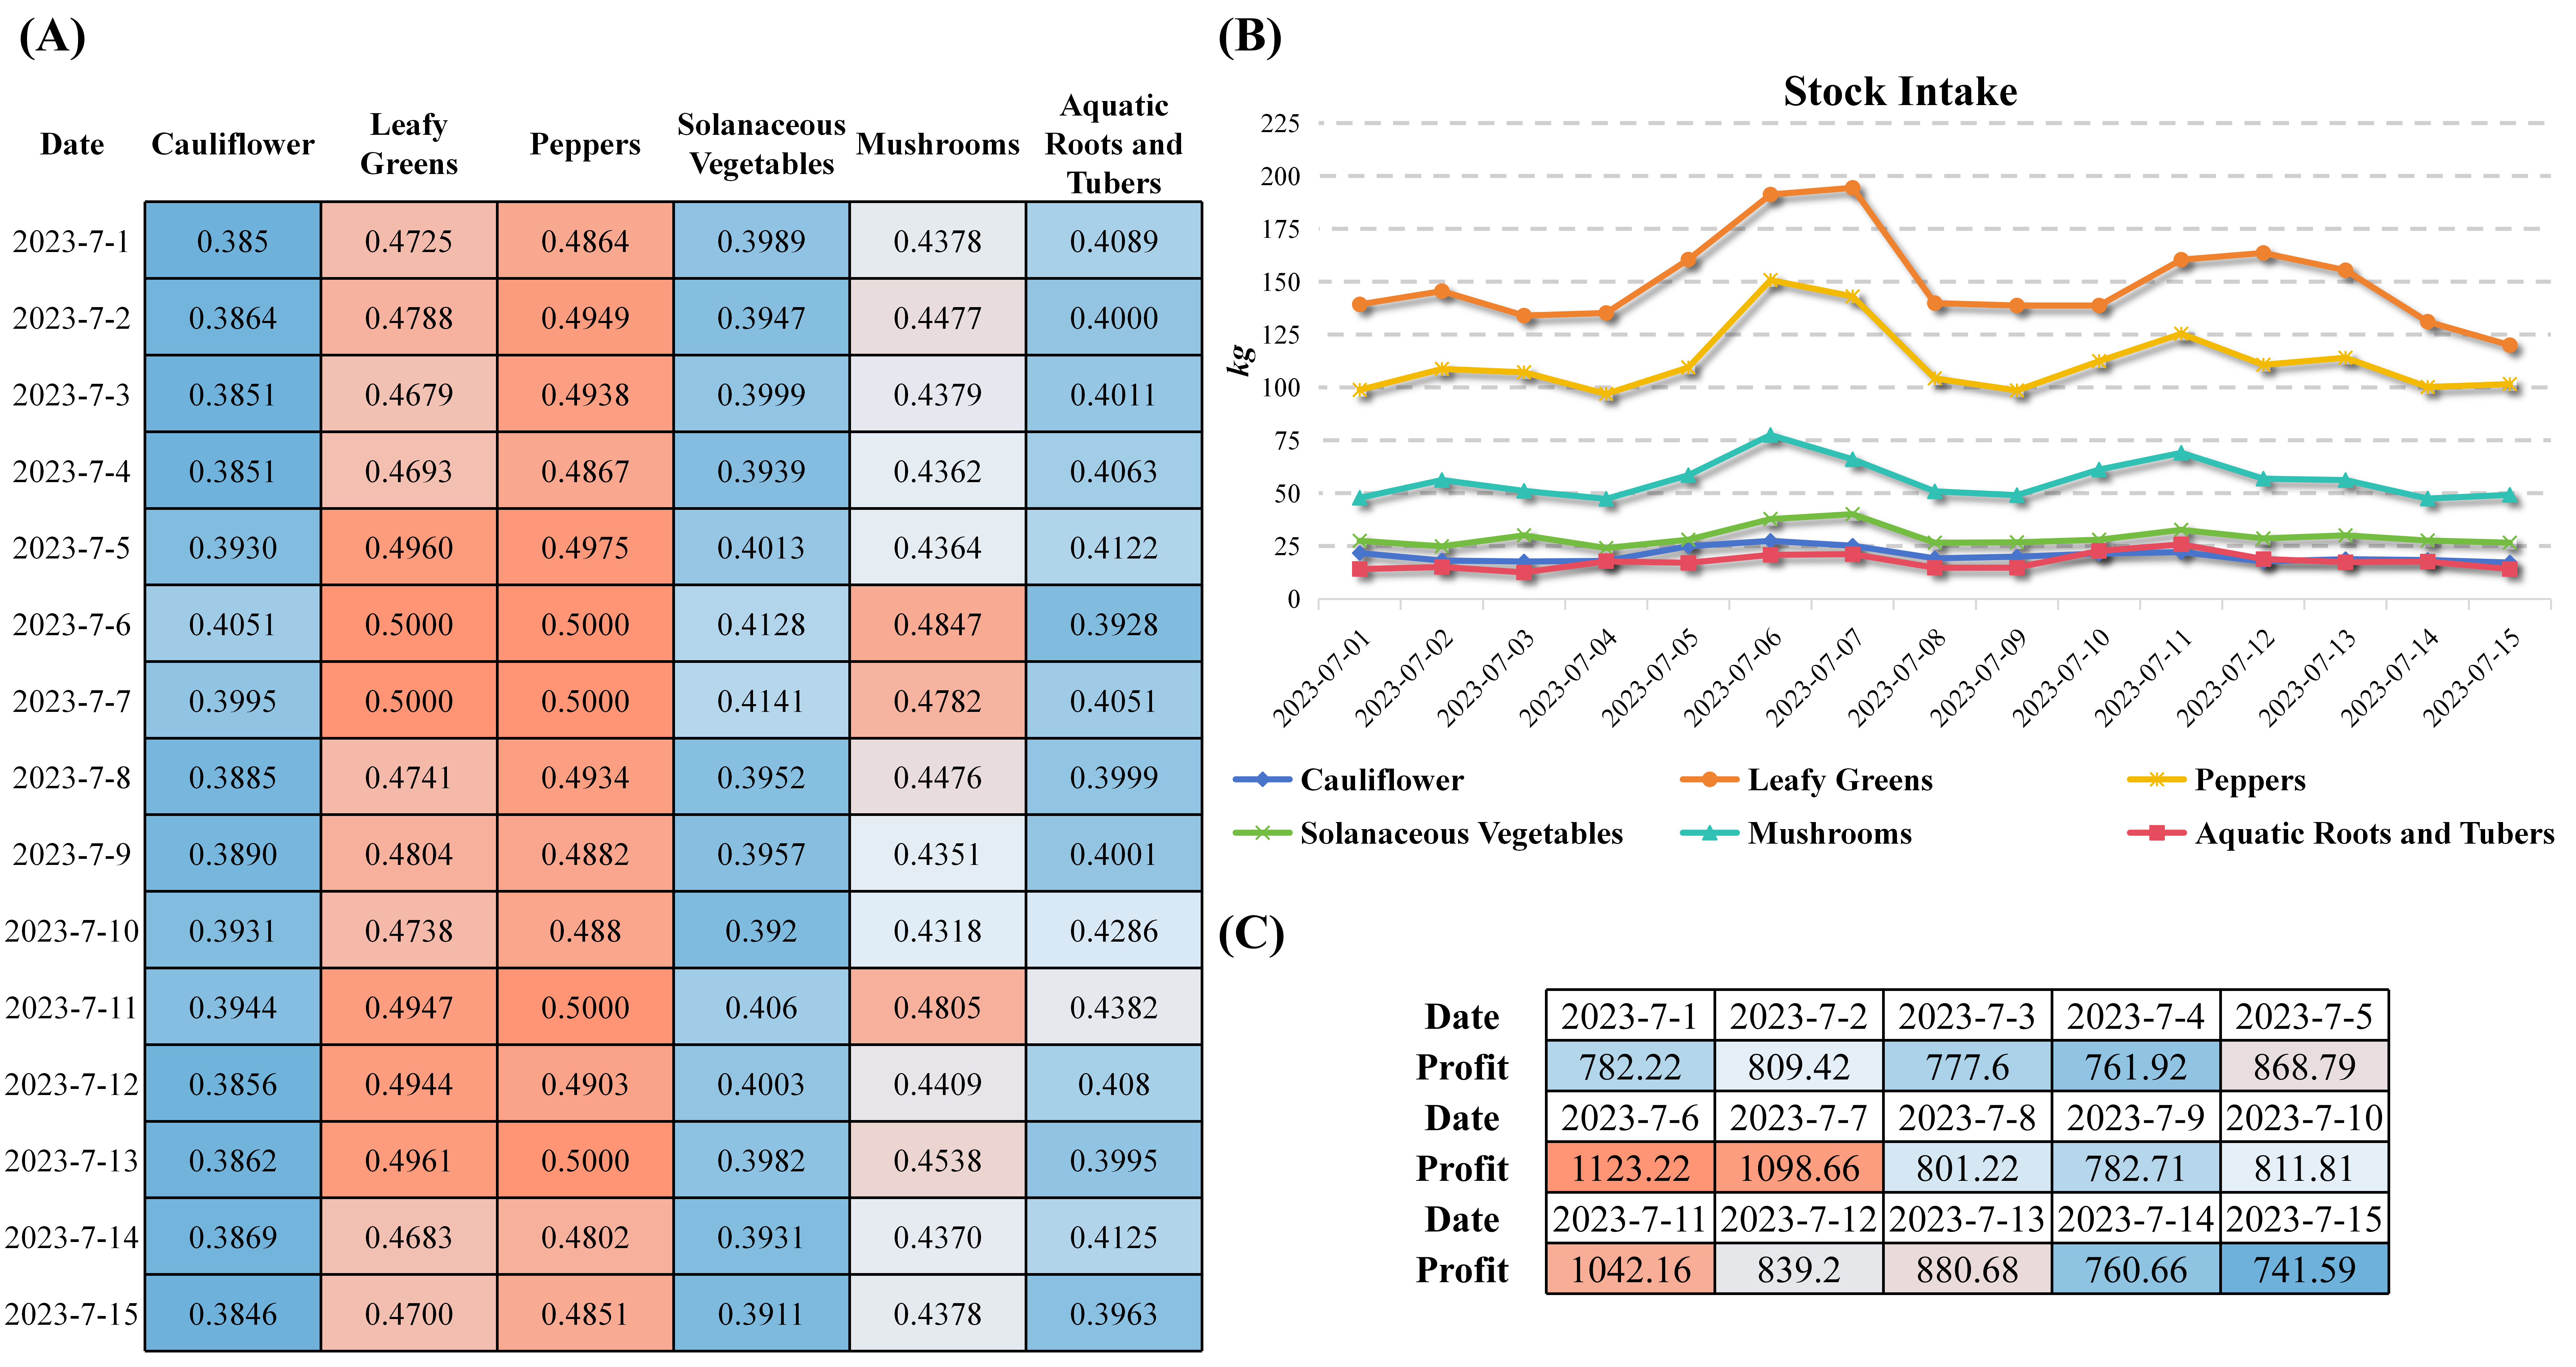
\includegraphics[width=1\textwidth]{图片6.png}
    \caption{未来15日超市运营决策结果。(A)定价加价率决策 (B)订货量决策 (C)农贸市场日利润}
    \label{fig:fig6}
\end{figure}

优化结果显示:加价率范围0.38-0.50,花菜类与水生块根类加价率较低,茄果类较高;日采购量呈波动特征,叶菜类采购量最高,水生块根类最低;超市日利润区间764.64-1123.22元,整体呈波动上升趋势,证实优化策略有效性。
\section{讨论与比较}
\label{sec:discussion_comparison}
本节探讨KAN-LSTM模型在农产品销量与价格预测中的性能表现,内容分为两部分:第\ref{subsec:ablation_study}节分析时序长期记忆的消融实验,第\ref{subsec:discussion_ordering_strategy}节讨论订货策略优化结果。

\subsection{时序长期记忆消融实验}
\label{subsec:ablation_study}

为验证KAN-LSTM模型的长期记忆能力,本研究将数据集划分为1年、2年、3年三种预测窗口,选取LSTM与xLSTM作为基准模型,评估不同预测跨度下模型的泛化性能。

\begin{table}[H]
  \centering
  \caption{不同时间窗口销量预测的KAN-LSTM消融实验}
  \label{tab:abl_sales}
  \resizebox{\textwidth}{!}{ 
  \begin{tabular}{lcccccccccc}
    \toprule
模型 &  & \multicolumn{3}{c}{\textbf{KAN-LSTM}} & \multicolumn{3}{c}{\textbf{xLSTM\citep{Beck2024}}} & \multicolumn{3}{c}{\textbf{LSTM\citep{Hochreiter1997}}} \\
\cmidrule(lr){3-5} \cmidrule(lr){6-8} \cmidrule(lr){9-11} 
指标 & 窗口 & \textbf{R2} & \textbf{RMSE} & \textbf{MAPE} & \textbf{R2} & \textbf{RMSE} & \textbf{MAPE} & \textbf{R2} & \textbf{RMSE} & \textbf{MAPE} \\
\midrule
    \multirow{3}{*}{花菜类} 
      & 365天 & \color{red}0.9769 & \color{red}3.5720 & \color{red}5.2679 & 0.9569 & 2.1479 & 7.3288 & 0.9320 & 2.6979 & 7.7506 \\
      & 730天 & \color{red}0.9710 & \color{red}3.1740 & \color{red}3.5875 & 0.9651 & 3.4821 & 2.7741 & 0.9346 & 4.7667 & 2.8250 \\
      & 1095天 & \textbf{\color{red}0.9903} & \textbf{\color{red}2.4215} & \textbf{\color{red}2.1889} & 0.9745 & 3.9370 & 4.2280 & 0.9335 & 6.3585 & 6.7969 \\
    \multirow{3}{*}{叶菜类} 
      & 365天 & \color{red}0.9018 & \textbf{\color{red}6.3052} & \color{red}1.9257 & 0.9421 & 11.2439 & 4.1950 & 0.9495 & 10.4983 & 3.1545 \\
      & 730天 & \color{red}0.9188 & \color{red}14.1301 & \color{red}1.6266 & 0.9285 & 21.3790 & 2.1547 & 0.9301 & 21.1357 & 1.7232 \\
      & 1095天 & \textbf{\color{red}0.9307} & \color{red}34.6191 & \textbf{\color{red}1.5977} & 0.8838 & 37.4981 & 2.6139 & 0.8695 & 39.7413 & 2.9743 \\
    \multirow{3}{*}{椒类} 
      & 365天 & \color{red}0.9673 & \color{red}7.1016 & \color{red}3.3214 & 0.9298 & 8.9425 & 2.6200 & 0.9271 & 9.1136 & 4.2099 \\
      & 730天 & \color{red}0.9508 & \color{red}12.6713 & \color{red}3.0132 & 0.9411 & 13.8579 & 4.2194 & 0.9330 & 14.7786 & 4.0132 \\
      & 1095天 & \textbf{\color{red}0.9864} & \textbf{\color{red}6.9606} & \textbf{\color{red}1.6975} & 0.9627 & 11.5436 & 6.6992 & 0.9552 & 12.6497 & 5.7077 \\
    \multirow{3}{*}{茄果类} 
      & 365天 & \color{red}0.9873 & \color{red}1.1469 & \textbf{\color{red}3.1911} & 0.9747 & 1.4785 & 3.8310 & 0.9559 & 1.9511 & 5.6651 \\
      & 730天 & \color{red}0.9865 & \color{red}1.3101 & \color{red}5.6574 & 0.9724 & 1.8717 & 8.7564 & 0.9599 & 2.2543 & 7.1288 \\
      & 1095天 & \textbf{\color{red}0.9912} & \textbf{\color{red}1.0600} & \color{red}5.9722 & 0.9536 & 2.4296 & 14.3475 & 0.9450 & 2.6457 & 26.3232 \\
    \multirow{3}{*}{食用菌类} 
      & 365天 & \color{red}0.9834 & \color{red}5.4062 & \color{red}3.1830 & 0.9660 & 4.8710 & 4.2744 & 0.9599 & 5.2907 & 3.8349 \\
      & 730天 & \color{red}0.9652 & \color{red}9.7093 & \color{red}2.6739 & 0.9632 & 9.9824 & 3.9105 & 0.9409 & 12.6473 & 2.7737 \\
      & 1095天 & \textbf{\color{red}0.9935} & \textbf{\color{red}2.1291} & \textbf{\color{red}1.0923} & 0.9315 & 5.2424 & 3.5220 & 0.9188 & 5.2639 & 3.1279 \\
    \multirow{3}{*}{水生块根类} 
      & 365天 & \color{red}0.9846 & \color{red}5.0668 & \color{red}5.5761 & 0.9470 & 1.9774 & 10.2619 & 0.9345 & 2.1975 & 13.3699 \\
      & 730天 & \color{red}0.9521 & \color{red}7.1925 & \color{red}5.6544 & 0.9202 & 9.2878 & 7.3120 & 0.9364 & 8.2901 & 4.3246 \\
      & 1095天 & \textbf{\color{red}0.9872} & \textbf{\color{red}4.0699} & \textbf{\color{red}5.5044} & 0.9750 & 5.6879 & 9.5540 & 0.9511 & 7.9602 & 16.6544 \\
    \bottomrule
  \end{tabular}
  }
\end{table}

\begin{table}[H]
  \centering
  \caption{不同时间窗口进货价格预测的KAN-LSTM消融实验}
  \label{tab:abl_prices}
  \resizebox{\textwidth}{!}{
  \begin{tabular}{lcccccccccc}
  \toprule
模型 & 窗口 & \multicolumn{3}{c}{\textbf{KAN-LSTM}} & \multicolumn{3}{c}{\textbf{xLSTM\citep{Beck2024}}} & \multicolumn{3}{c}{\textbf{LSTM\citep{Hochreiter1997}}} \\
\cmidrule(lr){3-5} \cmidrule(lr){6-8} \cmidrule(lr){9-11} 
指标 &  & \textbf{R2} & \textbf{RMSE} & \textbf{MAPE} & \textbf{R2} & \textbf{RMSE} & \textbf{MAPE} & \textbf{R2} & \textbf{RMSE} & \textbf{MAPE} \\
\midrule
    \multirow{3}{*}{花菜类} 
      & 365天 & \color{red}0.9604 & \color{red}0.1620 & \color{red}1.9586 & 0.9319 & 0.2125 & 1.3935 & 0.9257 & 0.2218 & 0.8013 \\
      & 730天 & \color{red}0.9565 & \color{red}0.2015 & \color{red}1.5385 & 0.9319 & 0.2519 & 1.8398 & 0.9446 & 0.2273 & 1.7983 \\
      & 1095天 & \textbf{\color{red}0.9752} & \textbf{\color{red}0.1378} & \textbf{\color{red}1.0163} & 0.9515 & 0.1930 & 1.1940 & 0.9203 & 0.2473 & 1.9973 \\
    \multirow{3}{*}{叶菜类} 
      & 365天 & \color{red}0.9830 & \textbf{\color{red}0.0639} & \color{red}1.6084 & 0.9451 & 0.1794 & 1.9208 & 0.9044 & 0.2366 & 3.3553 \\
      & 730天 & \color{red}0.9852 & \color{red}0.0942 & \color{red}1.7392 & 0.9629 & 0.1494 & 2.5803 & 0.9221 & 0.2164 & 3.4119 \\
      & 1095天 & \textbf{\color{red}0.9880} & \color{red}0.0977 & \textbf{\color{red}1.0796} & 0.9580 & 0.1826 & 3.8172 & 0.9144 & 0.2608 & 6.4929 \\
    \multirow{3}{*}{椒类} 
      & 365天 & \color{red}0.9501 & \color{red}0.1951 & \color{red}0.5621 & 0.9501 & 0.1063 & 0.6362 & 0.9036 & 0.1478 & 0.7433 \\
      & 730天 & \color{red}0.9511 & \color{red}0.1267 & \color{red}0.9111 & 0.9334 & 0.1479 & 1.2837 & 0.9345 & 0.1466 & 1.2799 \\
      & 1095天 & \textbf{\color{red}0.9517} & \textbf{\color{red}0.1161} & \textbf{\color{red}0.4079} & 0.9464 & 0.1224 & 1.5457 & 0.9368 & 0.1329 & 1.7060 \\
    \multirow{3}{*}{茄果类} 
      & 365天 & \color{red}0.9715 & \textbf{\color{red}0.1393} & \color{red}0.6615 & 0.9445 & 0.1943 & 1.1448 & 0.9459 & 0.1918 & 1.2810 \\
      & 730天 & \color{red}0.9548 & \color{red}0.1565 & \color{red}0.8651 & 0.9627 & 0.1422 & 1.2729 & 0.9214 & 0.2065 & 2.5518 \\
      & 1095天 & \textbf{\color{red}0.9756} & \color{red}0.1710 & \textbf{\color{red}0.5420} & 0.9577 & 0.2251 & 0.9828 & 0.9428 & 0.2618 & 1.2196 \\
    \multirow{3}{*}{食用菌类} 
      & 365天 & \color{red}0.9801 & \color{red}0.1311 & \color{red}1.6576 & 0.9564 & 0.1687 & 1.2552 & 0.9073 & 0.2460 & 1.6336 \\
      & 730天 & \color{red}0.9617 & \color{red}0.1843 & \color{red}1.3138 & 0.9331 & 0.2435 & 1.6365 & 0.9055 & 0.2893 & 2.0250 \\
      & 1095天 & \textbf{\color{red}0.9806} & \textbf{\color{red}0.1291} & \textbf{\color{red}1.0923} & 0.9315 & 0.2424 & 2.5220 & 0.9188 & 0.2639 & 3.1279 \\
    \multirow{3}{*}{水生块根类} 
      & 365天 & \color{red}0.9704 & \color{red}0.5750 & \color{red}1.8830 & 0.9524 & 0.7286 & 2.9308 & 0.9006 & 1.0527 & 4.9100 \\
      & 730天 & \color{red}0.9829 & \color{red}0.3734 & \color{red}1.8555 & 0.9540 & 0.6124 & 4.5322 & 0.9122 & 0.8461 & 5.4465 \\
      & 1095天 & \textbf{\color{red}0.9941} & \textbf{\color{red}0.1884} & \textbf{\color{red}1.4035} & 0.9608 & 0.4843 & 1.9060 & 0.9276 & 0.6588 & 4.0008 \\
    \bottomrule
  \end{tabular}
  }
\end{table}

表\ref{tab:abl_sales}与\ref{tab:abl_prices}显示:KAN-LSTM在所有时间窗口(365/730/1095天)均优于LSTM和xLSTM。花菜类销量预测中,KAN-LSTM的$R^2$值达0.9903(1095天窗口),显著高于对比模型;其RMSE与MAPE值也保持最低,验证预测准确性优势。

椒类销量预测在365天窗口下,KAN-LSTM的RMSE(7.1016)和MAPE(3.3214)均优于基准模型。特别在1095天长期预测中,KAN-LSTM展现更强的长期依赖捕捉能力:水生块根类进货价格预测$R^2$达0.9941,显著高于LSTM(0.9276)和xLSTM(0.9608),RMSE(0.1884)与MAPE(1.4035)改进幅度超30%。

结果表明:KAN-LSTM在长期时序预测中具有显著优势,能有效建模历史动态模式。1095天窗口验证集预测结果见图\ref{fig:fig7}-\ref{fig:fig8},其他窗口结果见附录C。

\begin{figure}[H]
    \centering
    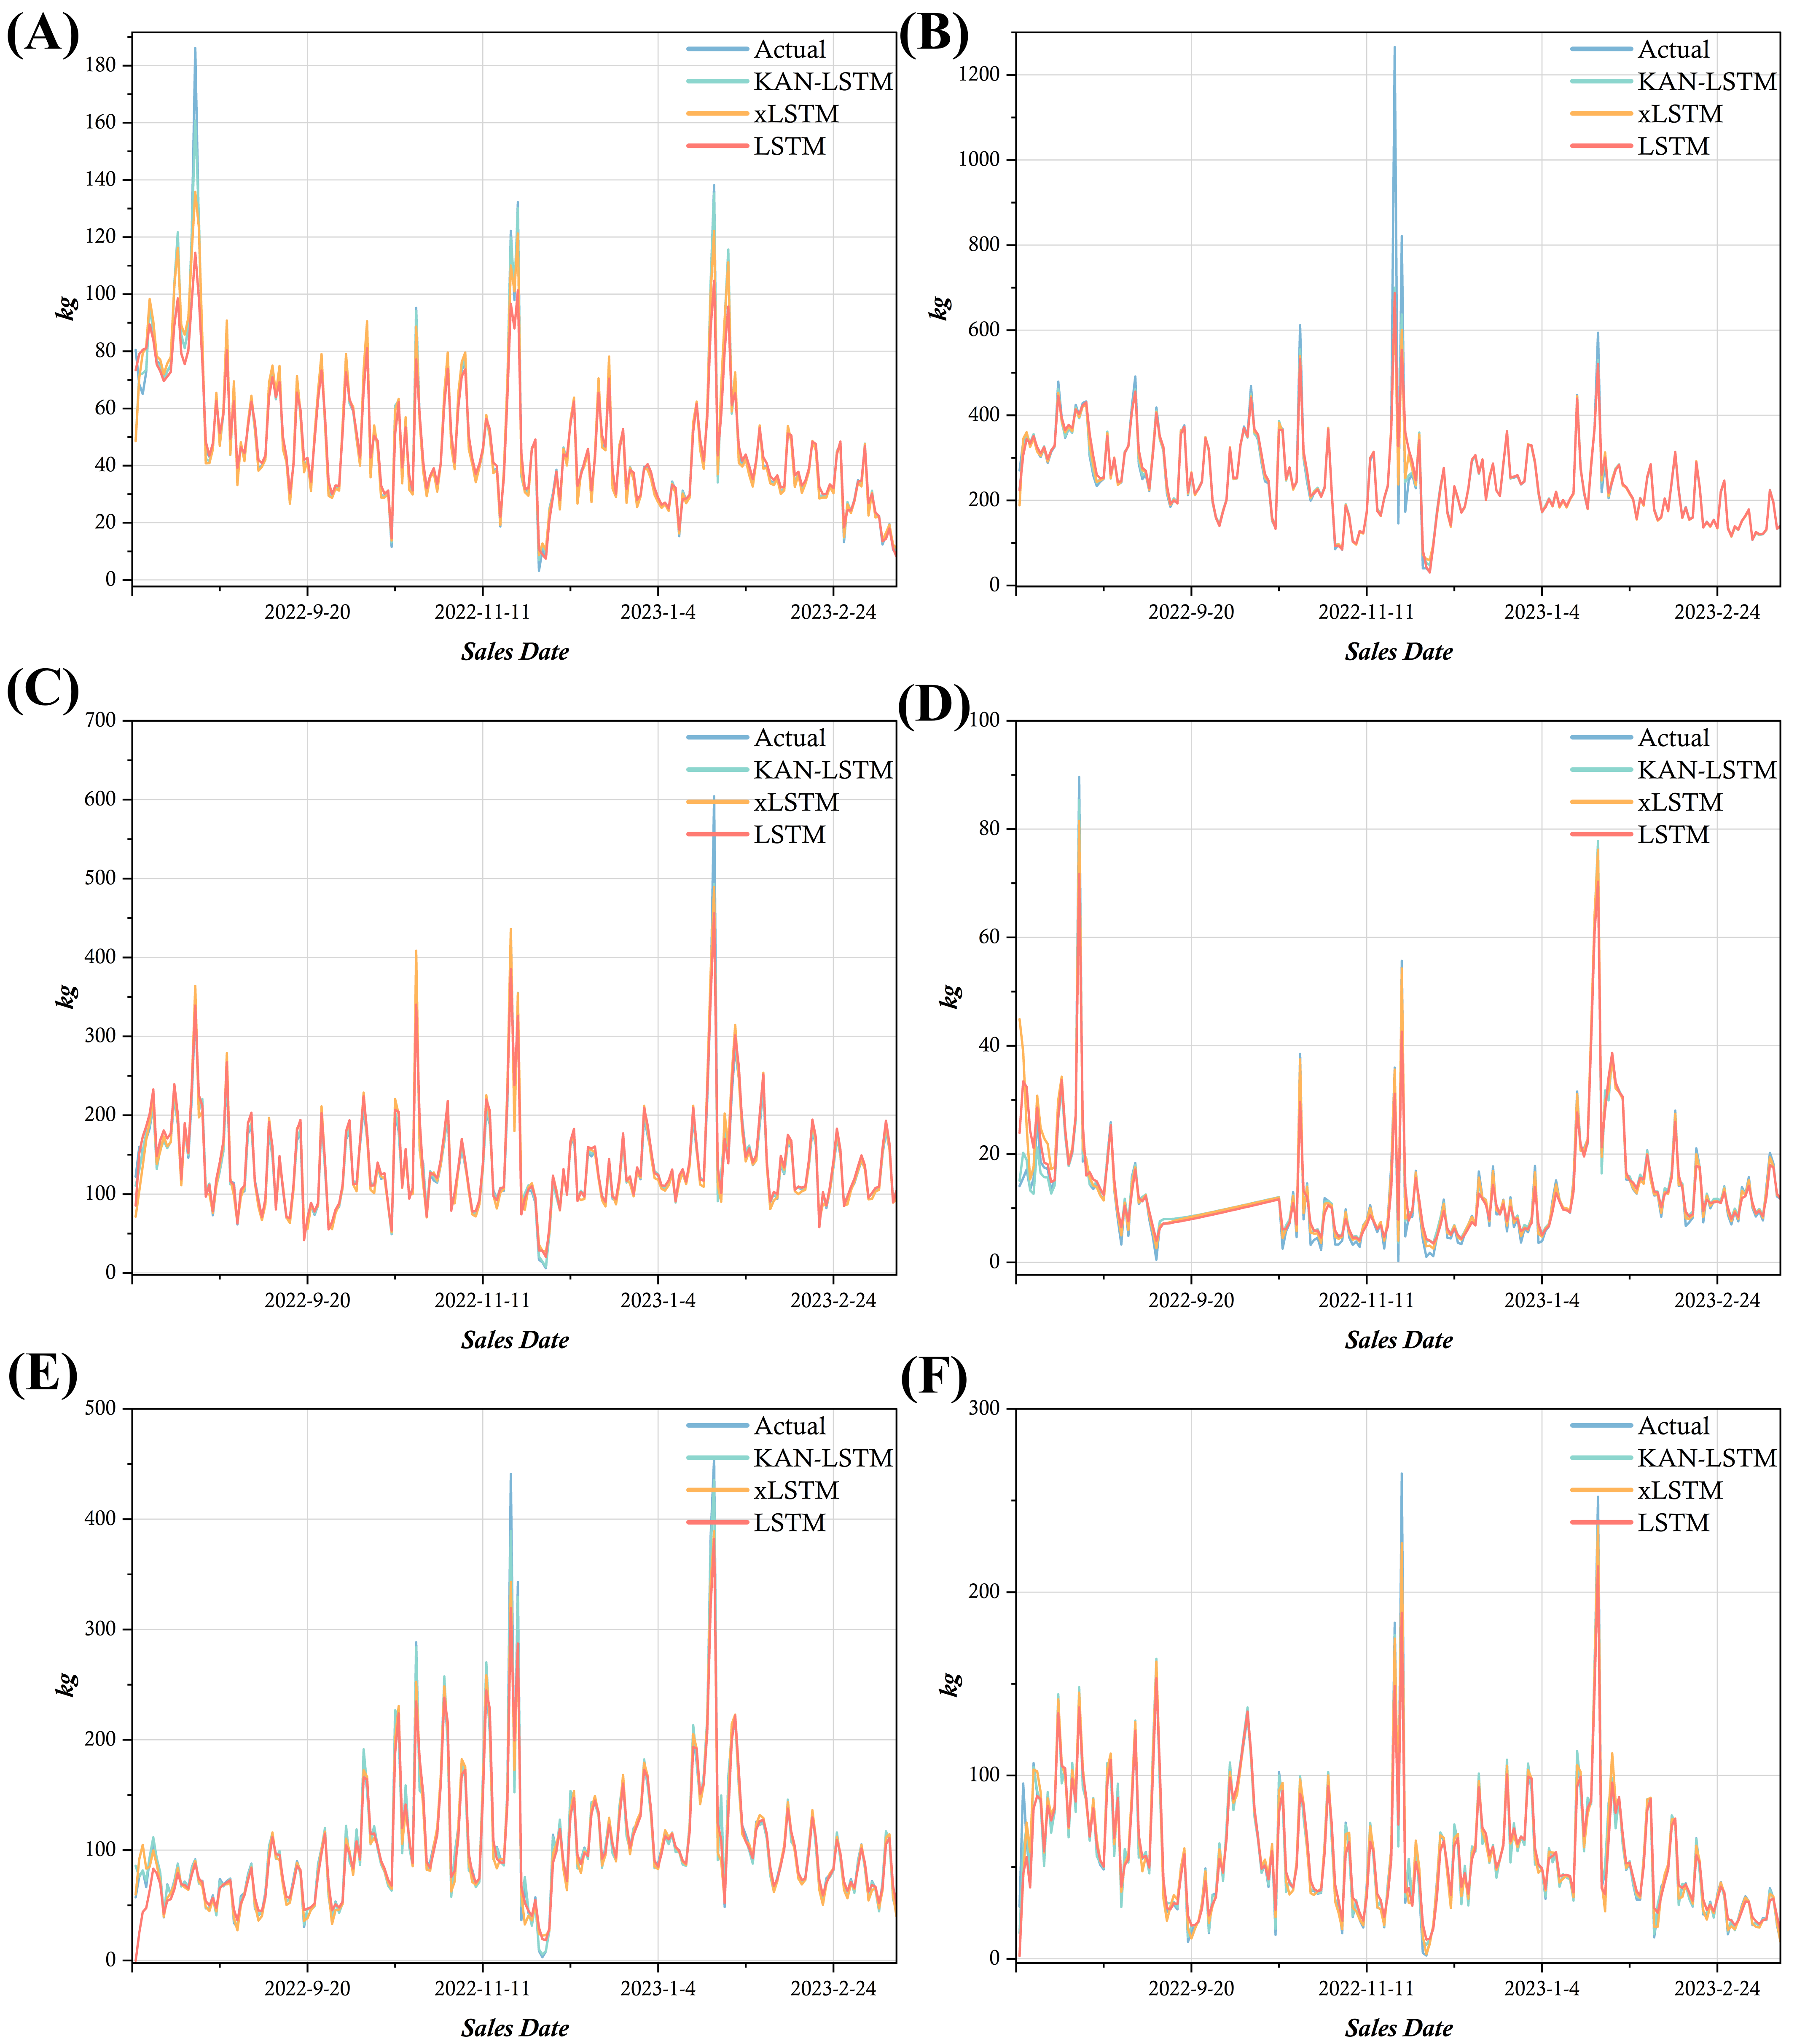
\includegraphics[width=1\textwidth]{图片7.png}
    \caption{1095天窗口销量预测结果。(A)-(F)依次为花菜类、叶菜类、椒类、茄果类、食用菌类、水生块根类}
    \label{fig:fig7}
\end{figure}

\begin{figure}[H]
    \centering
    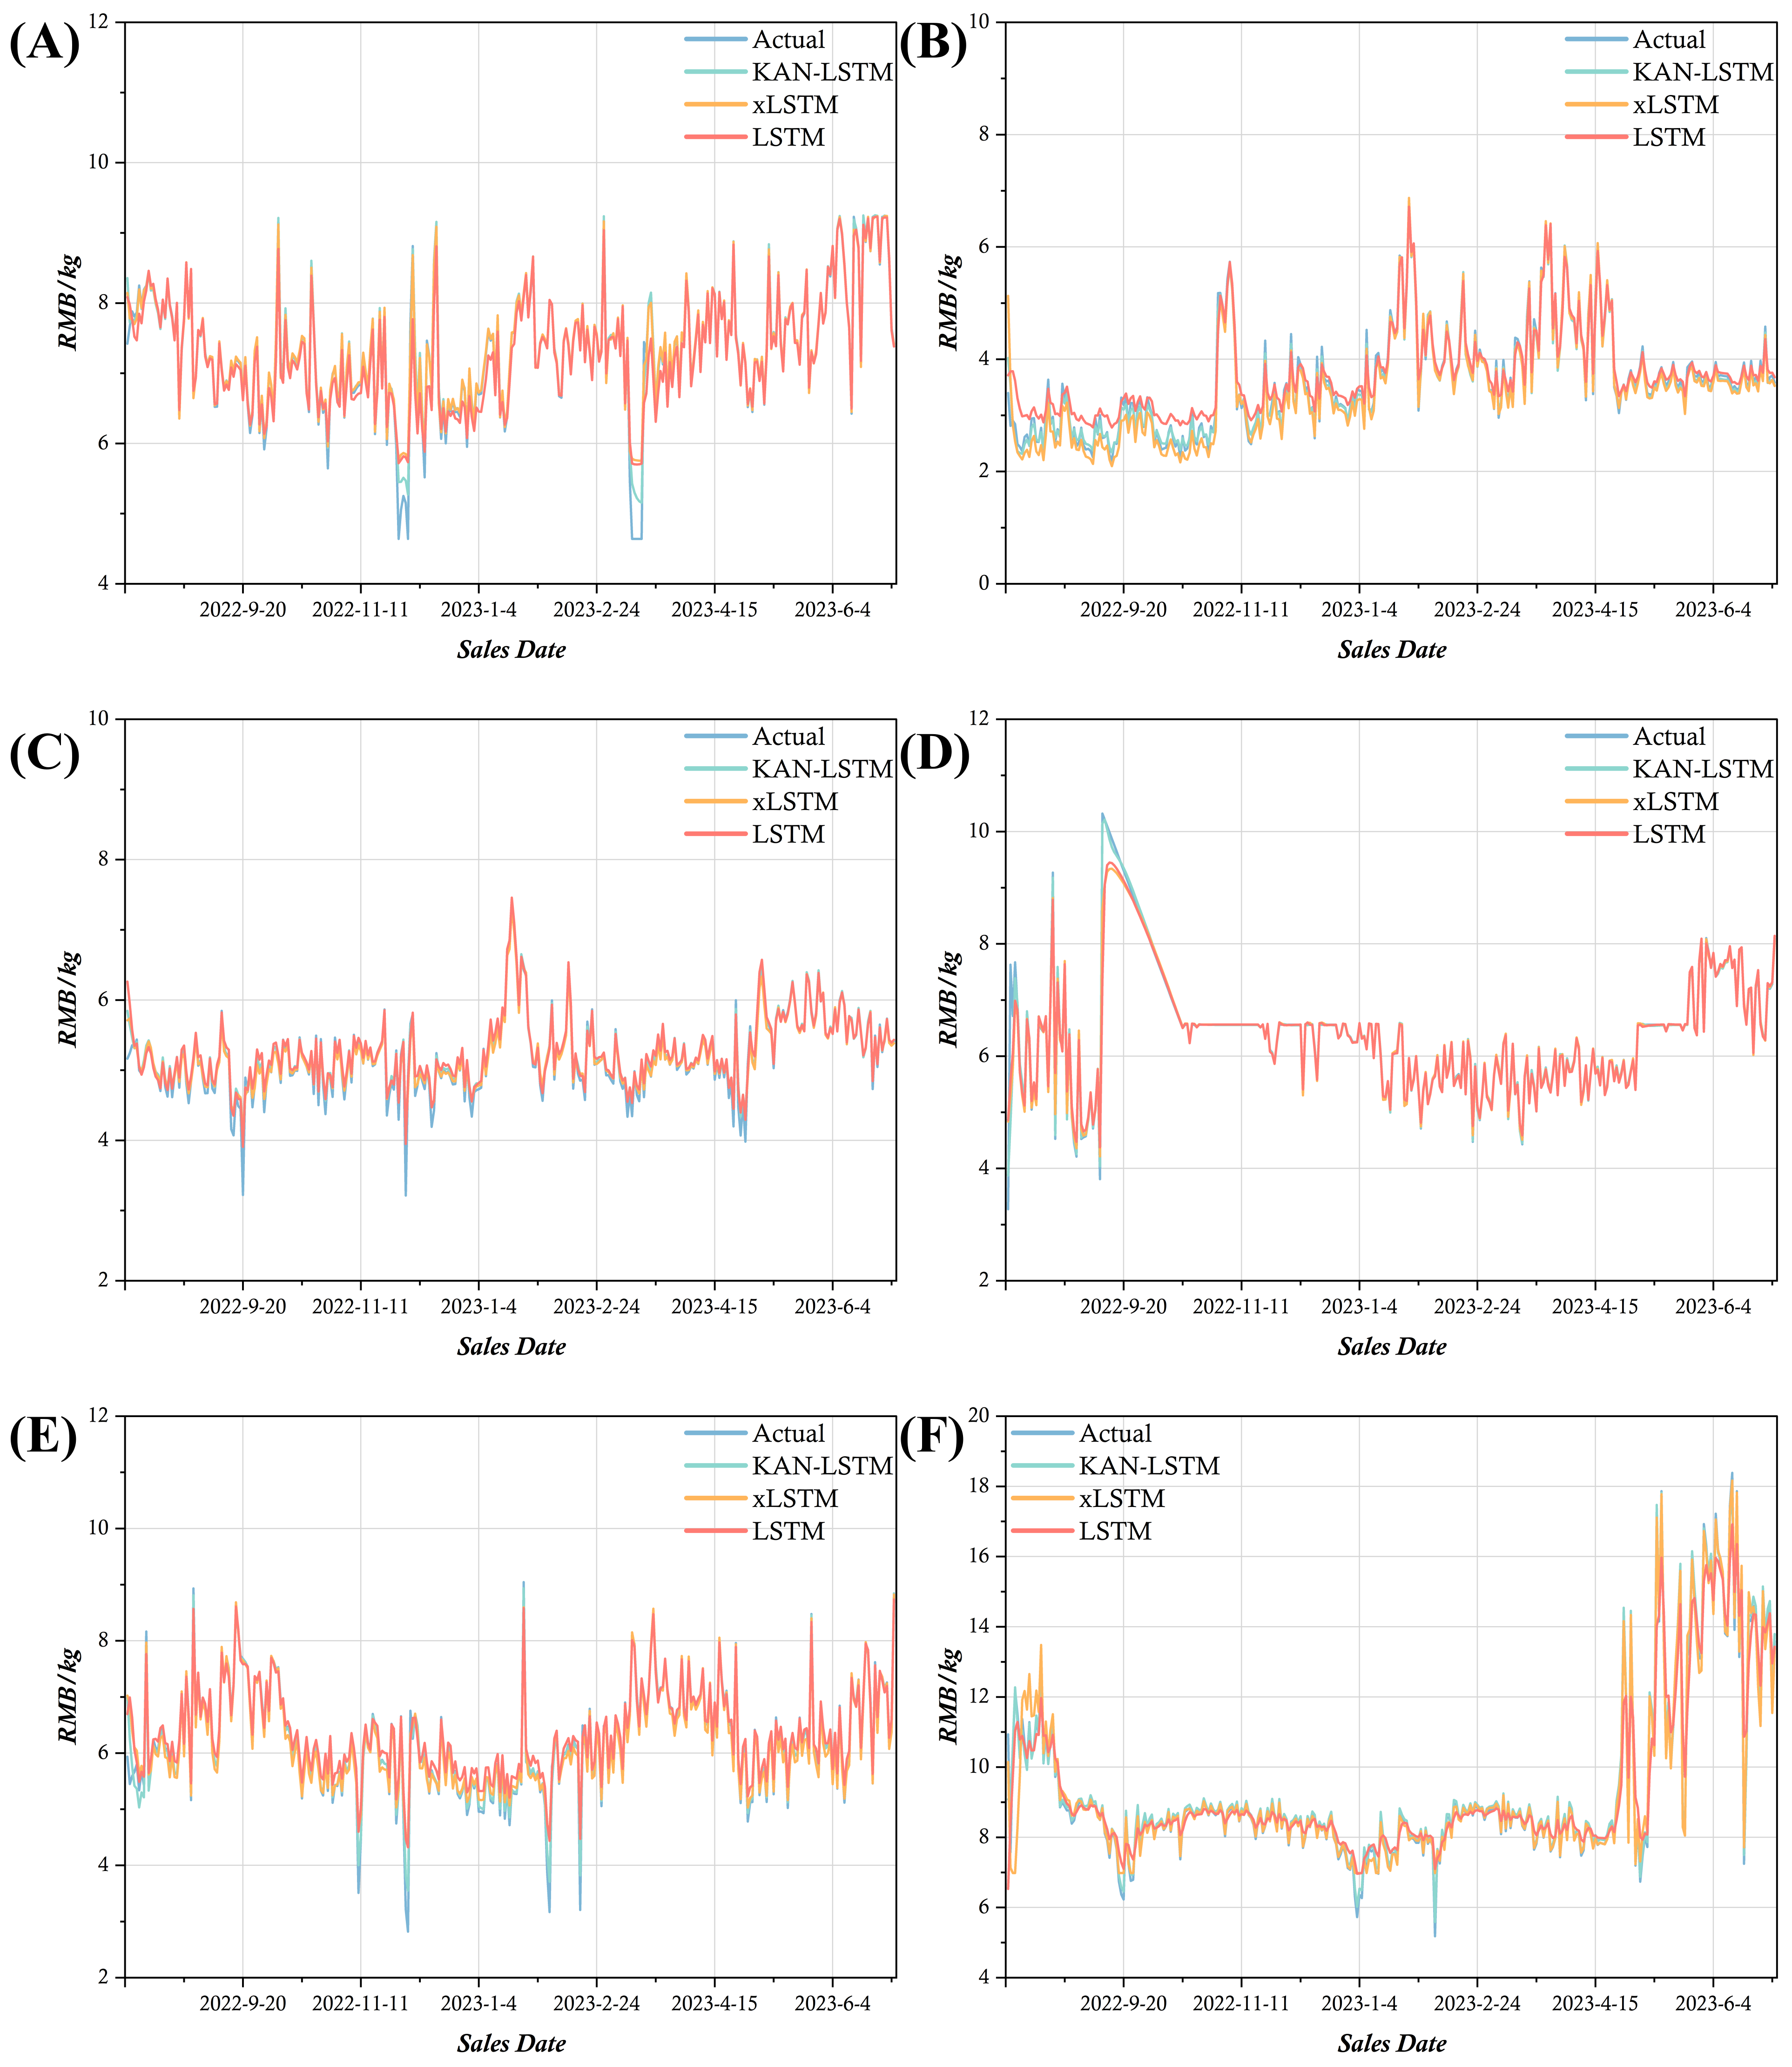
\includegraphics[width=1\textwidth]{图片8.png}
    \caption{1095天窗口进货价格预测结果。(A)-(F)品类顺序同图\ref{fig:fig7}}
    \label{fig:fig8}
\end{figure}

\subsection{订货策略优化讨论}
\label{subsec:discussion_ordering_strategy}

为分析模拟退火(SA)算法在求解非凸优化问题中的优势,选取粒子群优化(PSO)、遗传算法(GA)与禁忌搜索(TS)进行对比\citep{Kennedy1995,Alhijawi2024,Niroumandrad2024}。通过优化未来15日补货量与加价率,评估各算法求解多约束非线性规划的性能差异(图\ref{fig:fig9})。

结果显示:模拟退火(SA)、遗传算法(GA)与禁忌搜索(TS)优化结果相近,但GA与TS单次优化耗时高达3小时;粒子群优化(PSO)虽可在3分钟内完成,但解质量较差;SA算法兼顾优化效率与质量,单周期优化仅需约1分钟。这表明SA在时效敏感的实际决策场景中具有显著优势,特别适合需频繁调整的供应链动态优化问题。

\begin{figure}[H]
    \centering
    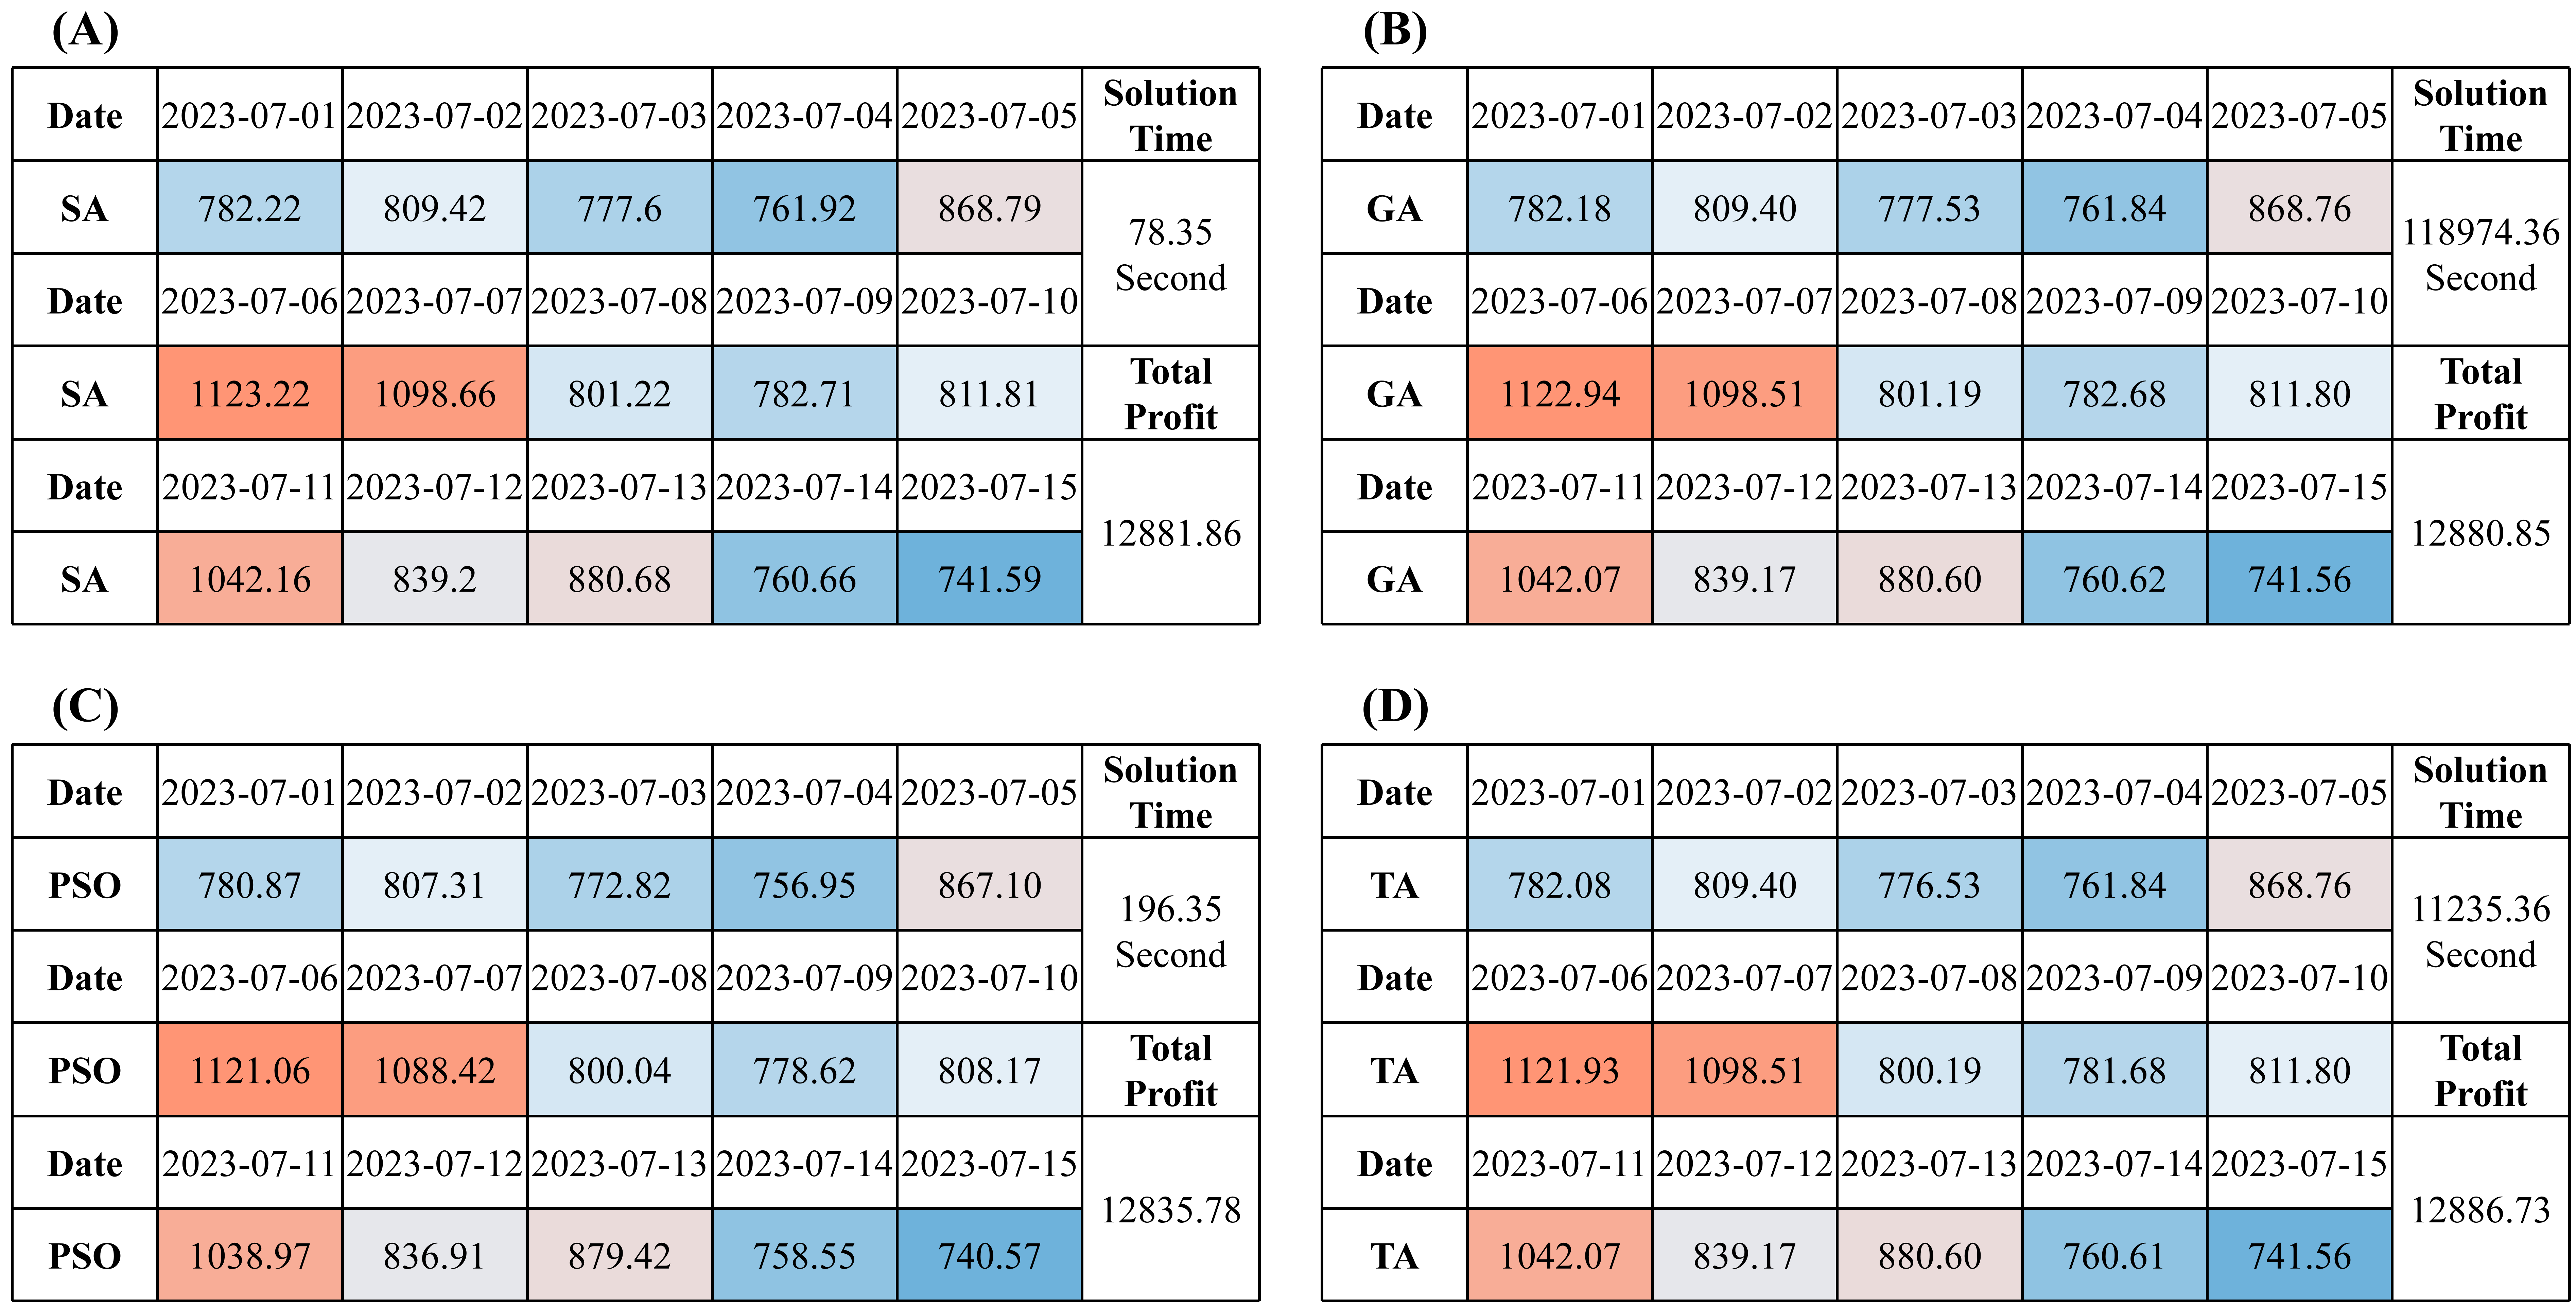
\includegraphics[width=1\textwidth]{图片9.png}
    \caption{优化算法性能比较。(A)SA算法 (B)GA算法 (C)PSO算法 (D)TS算法}
    \label{fig:fig9}
\end{figure}
\section{研究结论}
\label{sec:conclusions}

本文针对生鲜蔬菜产品的库存与定价策略优化问题,提出基于需求预测与优化决策的解决框架。通过多元逐步回归模型估计产品价格弹性与交叉弹性,建立融合产品成本、需求-价格关系及库存持有成本的需求预测模型,并采用KAN-LSTM深度学习模型实现需求时序预测。该模型展现优异的泛化能力,可有效捕捉复杂时序动态特征。

优化阶段运用模拟退火算法确定未来15日库存与加价策略,在保证解可行性与计算效率同时实现利润最大化。对比结果表明:模拟退火算法的计算效率显著优于其他算法(仅需1分钟),且优化结果稳定可靠。这些发现验证了框架有效性,为农产品市场库存定价决策提供科学依据,拓展了需求预测与优化算法在现实场景的应用潜力。

本研究存在一定局限性:首先未考虑损耗率($h$)随时间变化的动态特性;其次蔬菜补货与定价行为与天气、温度等自然因素存在关联,尽管历史数据已隐含此类信息,但显式引入自然变量能否进一步提升结果精度仍需深入探讨。
\newpage
\section*{数据可用性声明}
本研究数据通过\url{https://github.com/Zhanli-Li/Digital-Agricultural-Economics}公开访问,使用权限依据Apache-2.0 license。
\section*{AI辅助声明}
Copilot 用于辅助编写Python代码,我已检查代码并确保其正确性。ChatGPT 和 DeepSeek 用于辅助润色文章和检查语病,我已检查内容并确保其正确性。代码或内容中的任何错误由我本人负责。
\newpage
\newpage
\nocite{*}
\printbibliography[heading=bibintoc, title=\ebibname]
\newpage
\appendix
%\appendixpage
\addappheadtotoc
\section{附录:KAN网络架构}
\label{sec:appendix_kan}

柯尔莫哥洛夫-阿诺德表示定理表明:任意多元连续函数$f(x_1, x_2, \ldots, x_n)$可表示为一元函数的叠加与复合\citep{Braun2009},即:
\begin{equation}
f(x_1, \ldots, x_n) = \sum_{q=1}^{2n+1} \Phi_q \left( \sum_{p=1}^n \phi_{q,p}(x_p) \right),
\end{equation}
其中$\phi_{q,p} : [0,1] \rightarrow \mathbb{R}$为一元映射函数,$\Phi_q : \mathbb{R} \rightarrow \mathbb{R}$为另一组一元映射函数。

\begin{figure}[H]
        \centering
        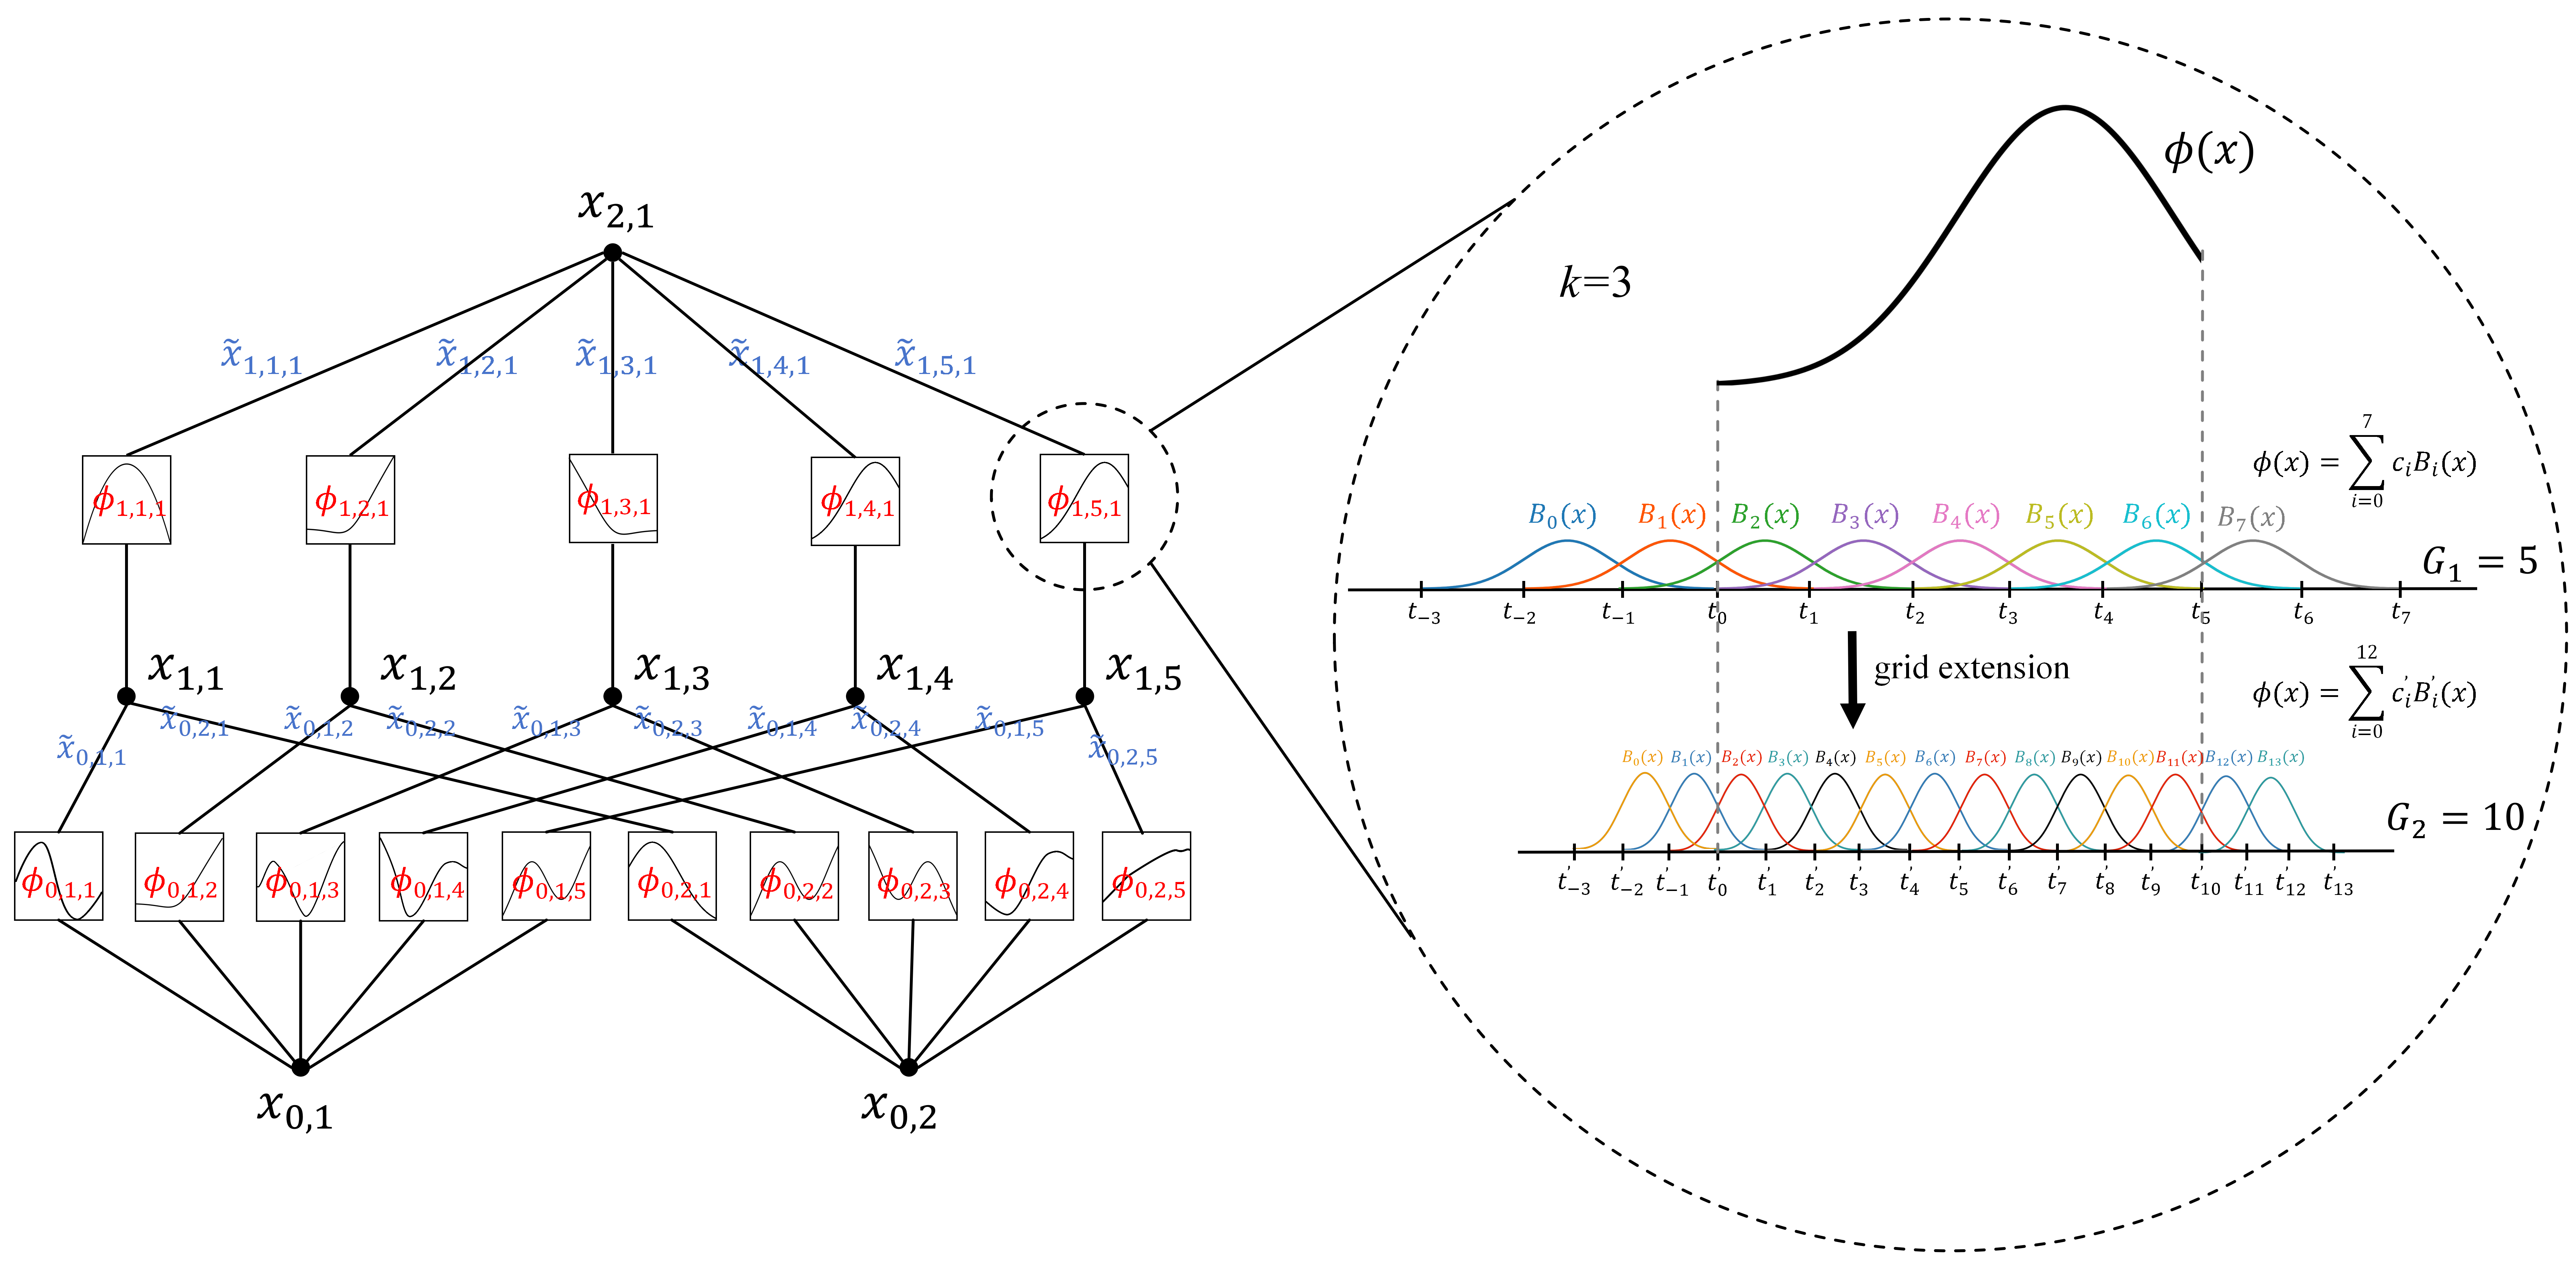
\includegraphics[width=1\textwidth]{图片14.png}
        \caption{KAN架构运行机理}
        \label{fig:fig14}
\end{figure}
如图\ref{fig:fig14}所示,KAN网络架构基于该理论,在神经网络连接处学习激活函数而非使用传统固定激活函数(如ReLU、Sigmoid)。KAN网络中每层计算式为:
\begin{equation}
x_{l+1,j} = \sum_{i=1}^{n_l} \phi_{l,j,i}(x_{l,i}),
\end{equation}
可表示为:
\begin{equation}
x_{l+1} = \Phi_l x_l,
\end{equation}
其中$\Phi_l$表示KAN网络的函数矩阵。KAN网络整体计算表示为:
\begin{equation}
KAN(x) = (\Phi_L \circ \Phi_{L-1} \circ \cdots \circ \Phi_1 \circ \Phi_0) x.
\end{equation}
该架构赋予KAN更强的非线性建模能力与优越的函数逼近特性。

\section{附录:定理1证明}
\label{sec:appendix_proof}
为证明本文定理,需引入以下引理:
\label{sec:proof}
\begin{lemma}[复合函数凹凸性传递规则]
        若$f(x)$为凹函数且$g(x)$单调递增,则$f(g(x))$仍为凹函数;若$f(x)$为凸函数且$g(x)$单调递增,则$f(g(x))$仍为凸函数。
    \end{lemma}
    
    \begin{lemma}[单调函数与凹凸函数的乘积规则]
        设$f(x)$为凸函数,$g(x)$为单调递增线性函数,则乘积函数$h(x) = f(x) g(x)$为凸函数;若$f(x)$为凹函数,$g(x)$为单调递增线性函数,则$h(x)$为凹函数。
    \end{lemma}
    
    \begin{lemma}[线性函数的凹凸性传递]
        给定函数$g(x)$与线性函数$h(x) = ax + b$:若$g(x)$为凹函数,则$f(x) = g(x) - h(x)$仍为凹函数;若$g(x)$为凸函数,则$f(x) = g(x) - h(x)$仍为凸函数。
    \end{lemma}

首先解析本文目标函数与约束条件。目标函数包含利润项与成本项两部分。根据引理1,仅需分别论证两部分函数的凹凸性。

\textbf{利润函数}
利润定义为:
\begin{equation}
f_1(Q, m) = \sum_i c_i m_i D_i
\end{equation}
其中$c_i m_i$为线性递增函数,不改变凹凸性。因需求函数$D_i$与$m_i$呈非线性关系,由引理2,$f_1(Q, m)$的凹凸性取决于需求函数$D_i$的凹凸性。

\textbf{成本函数}
成本定义为:
\begin{equation}
f_2(Q, m) = \sum_i h_i (D_i - Q_i)
\end{equation}
此处$Q_i$为线性变量,不改变凹凸性。因$D_i$与$m_i$的非线性关系,由引理3,成本函数$f_2(Q, m)$的凹凸性与$D_i$保持一致。

\textbf{约束条件}
库存约束$Q_i \geq D_i$:若$D_i$为凸函数,则$Q_i \geq D_i$定义的集合为凸集;反之若$D_i$为非凸函数,则该约束定义非凸集。
加价率约束$m_{\min} \leq m_i \leq m_{\max}$为线性约束,其定义的集合为凸集。

综上,目标函数与约束条件的凹凸性完全取决于$D_i$的凹凸性。

\textbf{需求函数凹凸性分析}
需求函数$D_i$形式为:
\begin{equation}
D_i = e^{\alpha_i} \left[ c_i (1 + m_i) \right]^{-\beta_i} \prod_j p_j^{\gamma_{ij}} \prod_j D_j^{\delta_{ij}}
\end{equation}
因$p_j^{\gamma_{ij}}$不直接依赖$m_i$,且$D_j^{\delta_{ij}}$与$m_i$关系需递归求解,现仅考虑$D_i$对$m_i$的二阶特性。$D_i$对$m_i$的一阶与二阶导数为:
\begin{equation}
\frac{\partial D_i}{\partial m_i} = -\beta_i e^{\alpha_i} \left[ c_i (1 + m_i) \right]^{-\beta_i - 1} c_i \prod_j p_j^{\gamma_{ij}} \prod_j D_j^{\delta_{ij}}
\end{equation}
\begin{equation}
\frac{\partial^2 D_i}{\partial m_i^2} = \beta_i (\beta_i + 1) e^{\alpha_i} \left[ c_i (1 + m_i) \right]^{-\beta_i - 2} c_i^2 \prod_j p_j^{\gamma_{ij}} \prod_j D_j^{\delta_{ij}}
\end{equation}

当$\beta_i (\beta_i + 1) \geq 0$时,$\frac{\partial^2 D_i}{\partial m_i^2} \geq 0$,$D_i$为凸函数;当$\beta_i (\beta_i + 1) < 0$时,$\frac{\partial^2 D_i}{\partial m_i^2} < 0$,$D_i$为凹函数。

故$D_i$在$\beta_i \geq 0$或$\beta_i \leq -1$时为凸函数,在$-1 < \beta_i < 0$时为凹函数。

\textbf{定理得证}
优化问题为凸优化问题当且仅当所有$D_i$均为凸函数。具体而言,当$\beta_i (\beta_i + 1) \geq 0$(即$\beta_i \geq 0$或$\beta_i \leq -1$)时满足凸性条件;当$-1 < \beta_i < 0$时问题为非凸。

\section{附录:附加图表}
\label{sec:appendix_figures}

\begin{figure}[H]
    \centering
    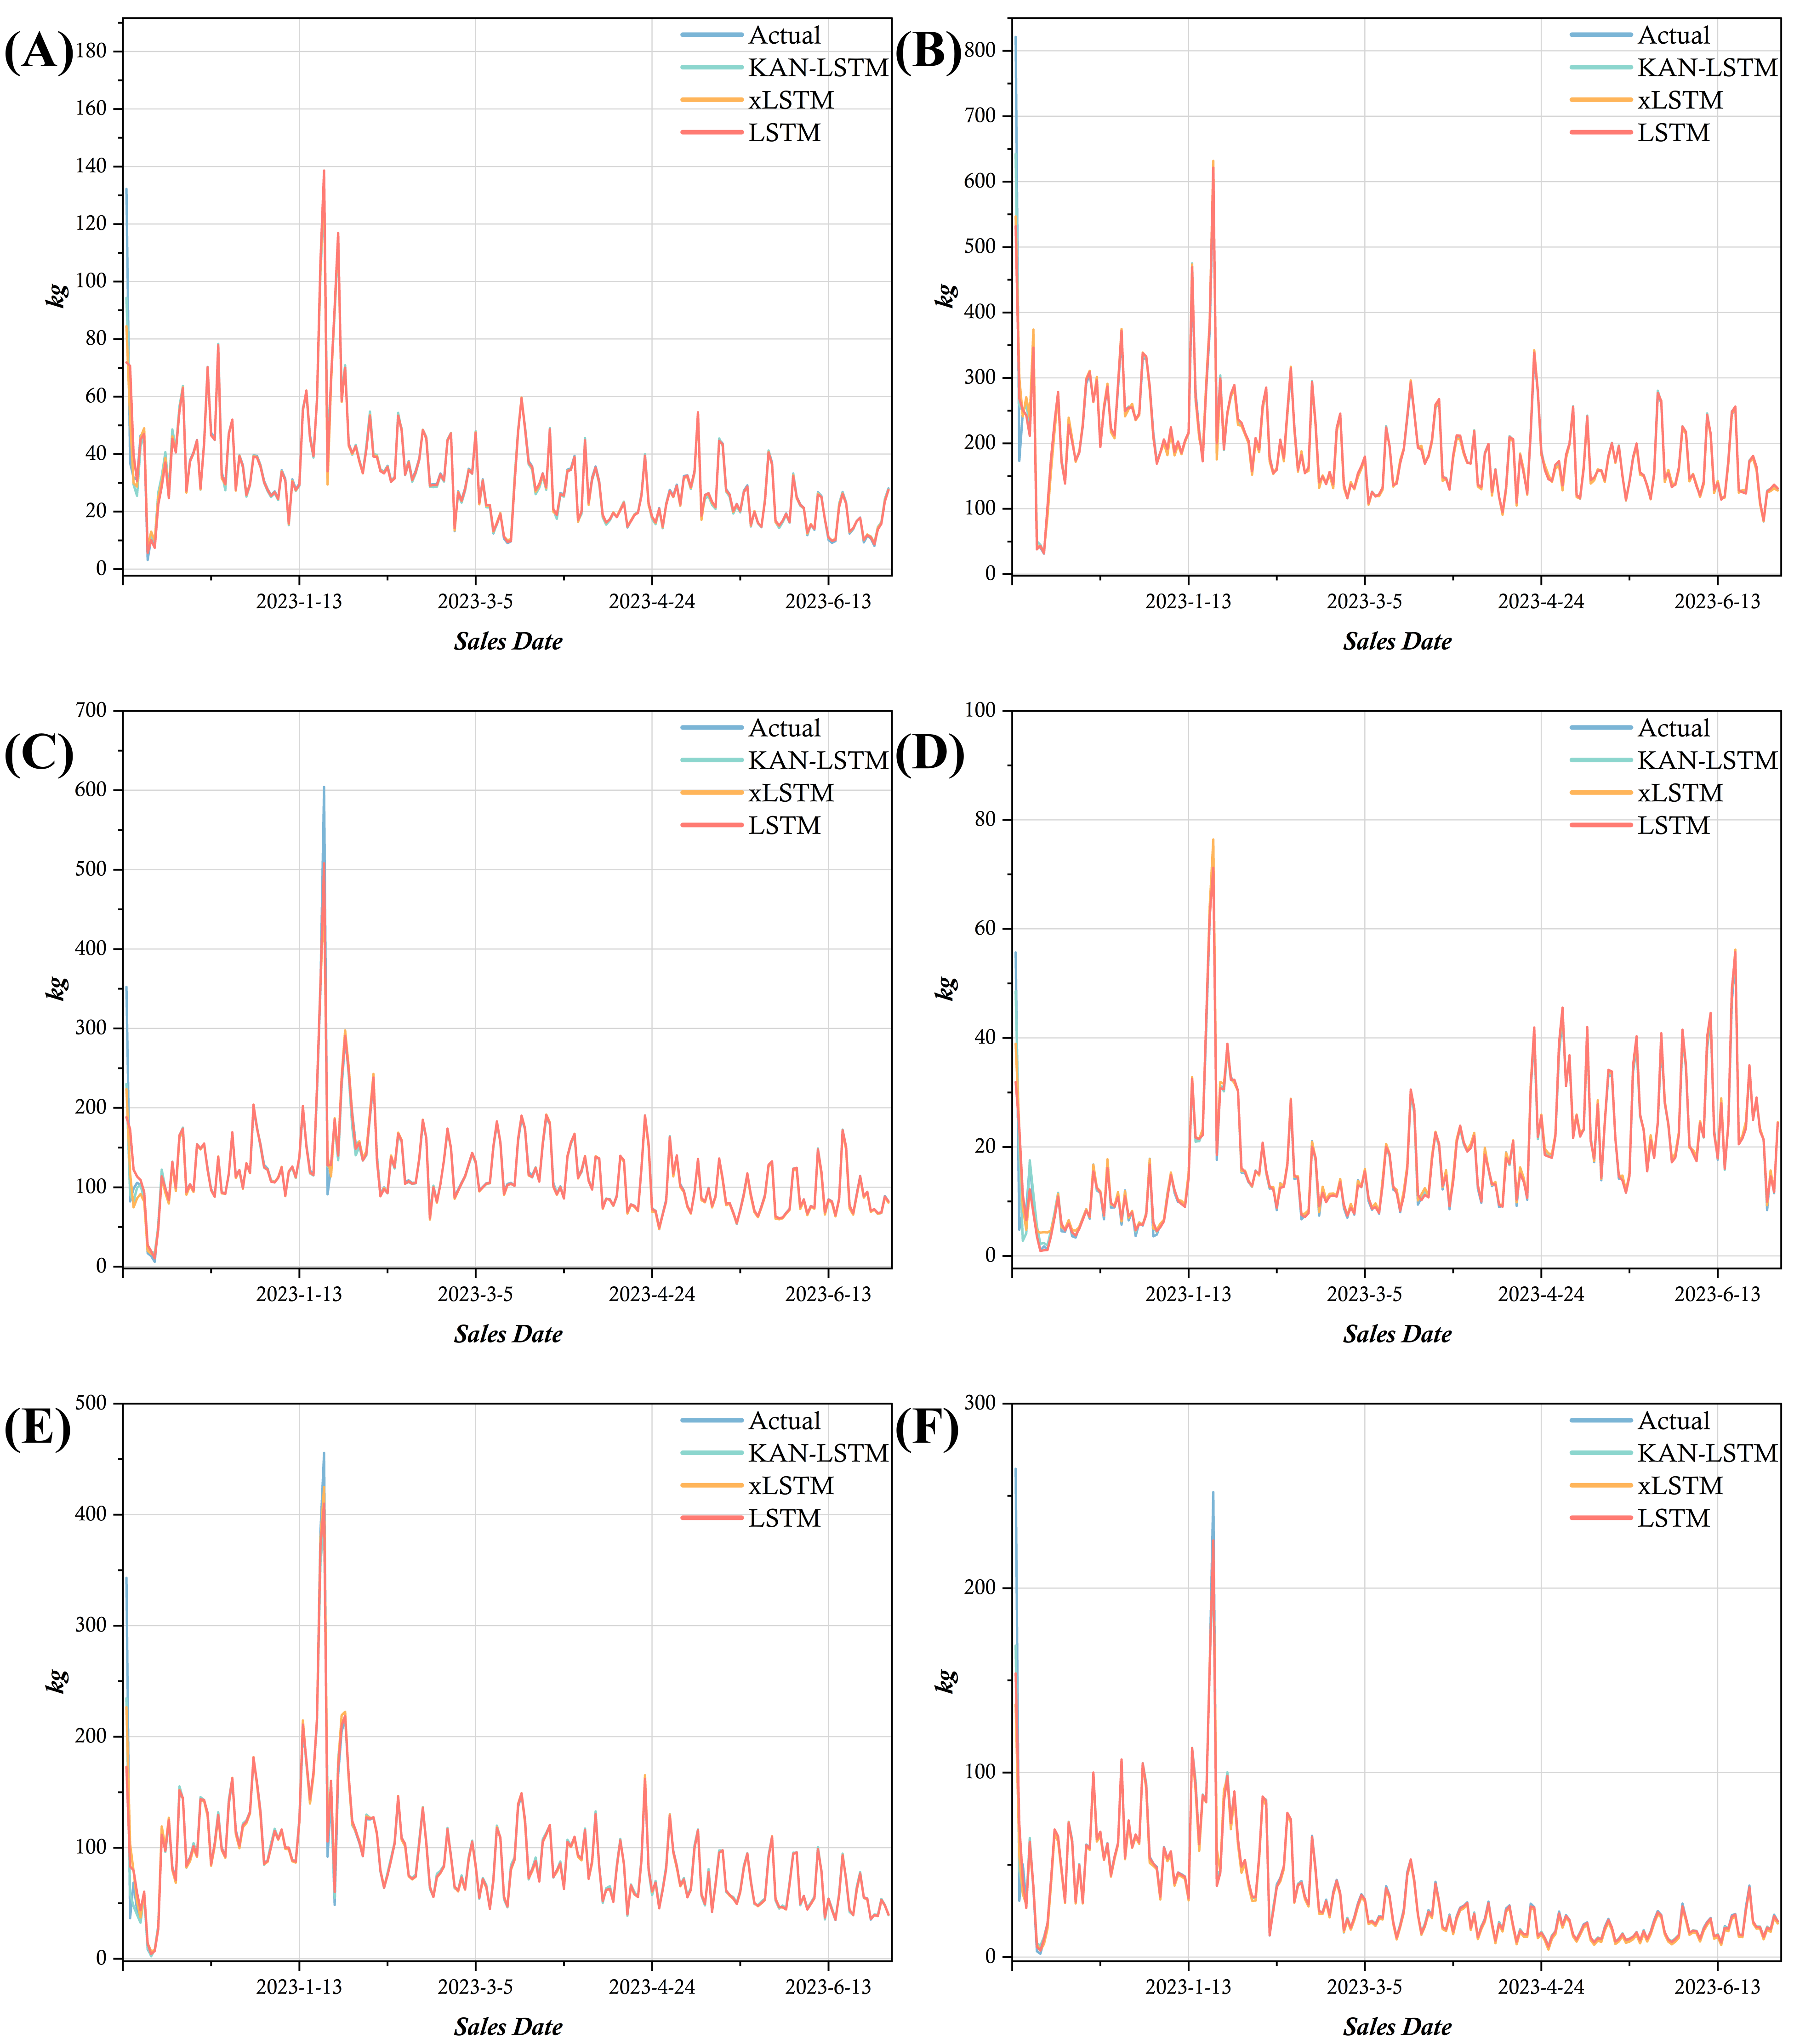
\includegraphics[width=1\textwidth]{图片10.png}
    \caption{730天窗口销量预测结果。(A)-(F)依次为花菜类、叶菜类、椒类、茄果类、食用菌类、水生块根类}
    \label{fig:fig10}
\end{figure}

\begin{figure}[H]
    \centering
    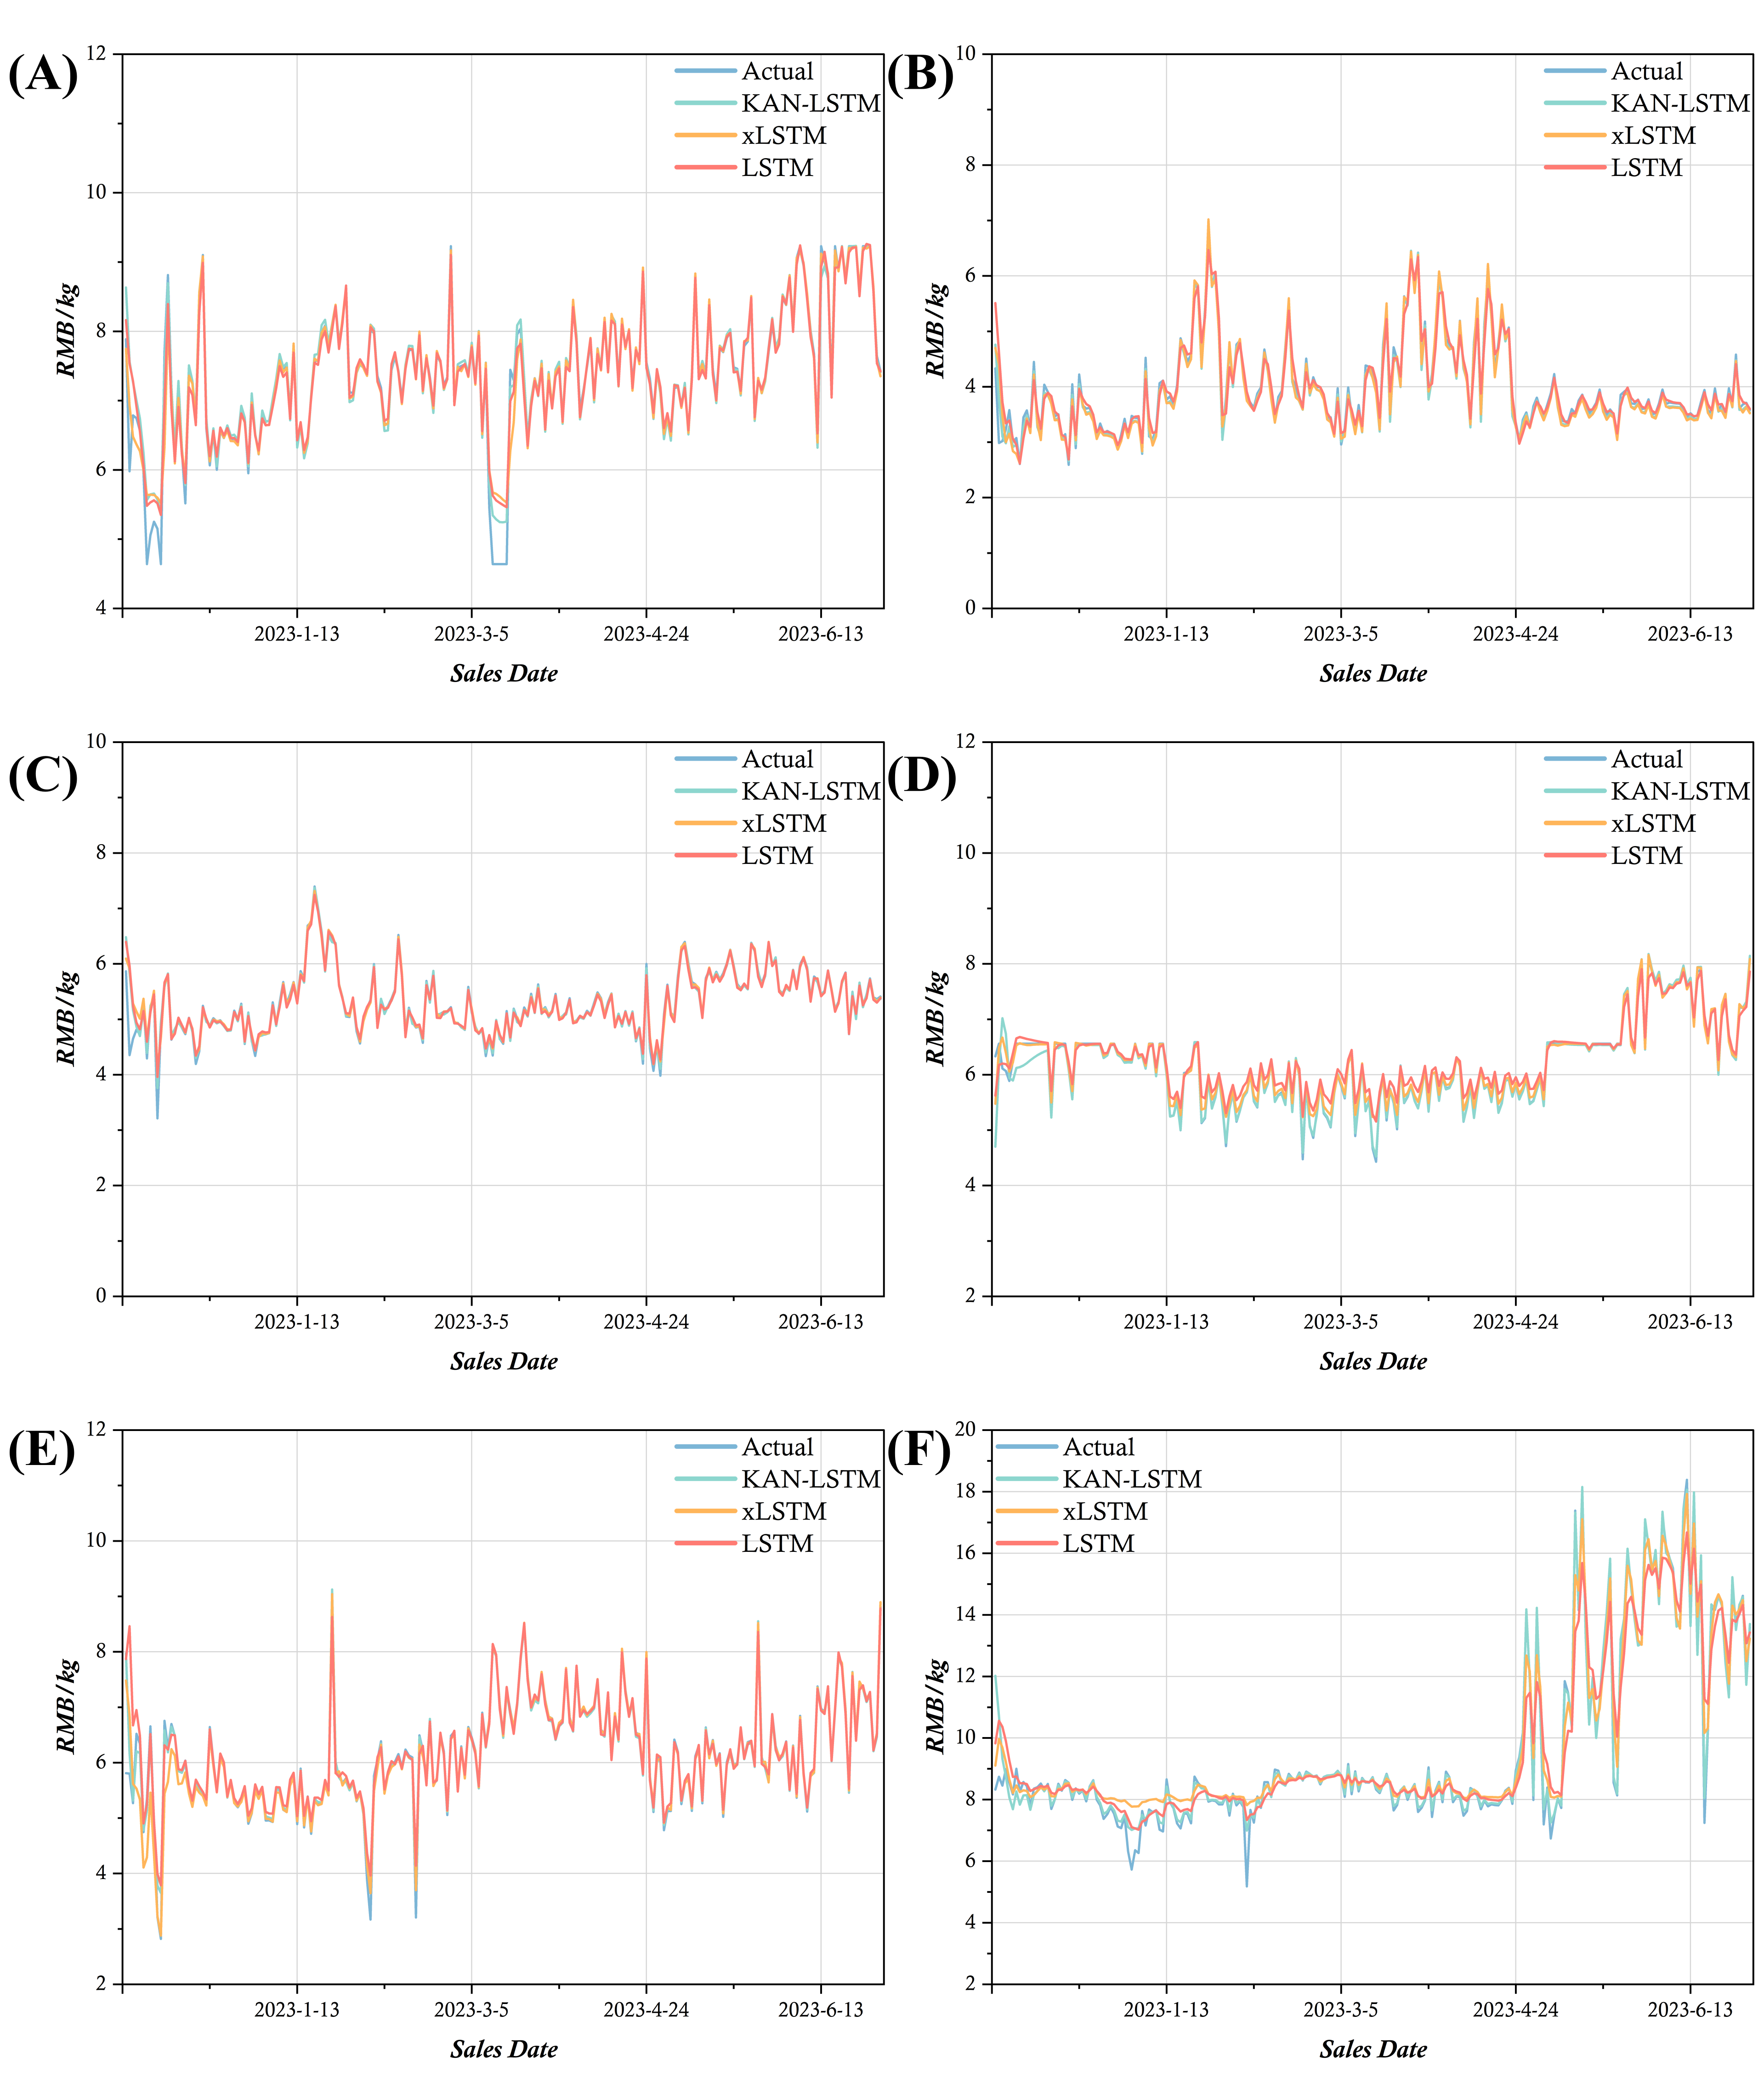
\includegraphics[width=1\textwidth]{图片11.png}
    \caption{730天窗口进货价格预测结果。(A)-(F)品类顺序同图\ref{fig:fig10}}
    \label{fig:fig11}
\end{figure}

\begin{figure}[H]
    \centering
    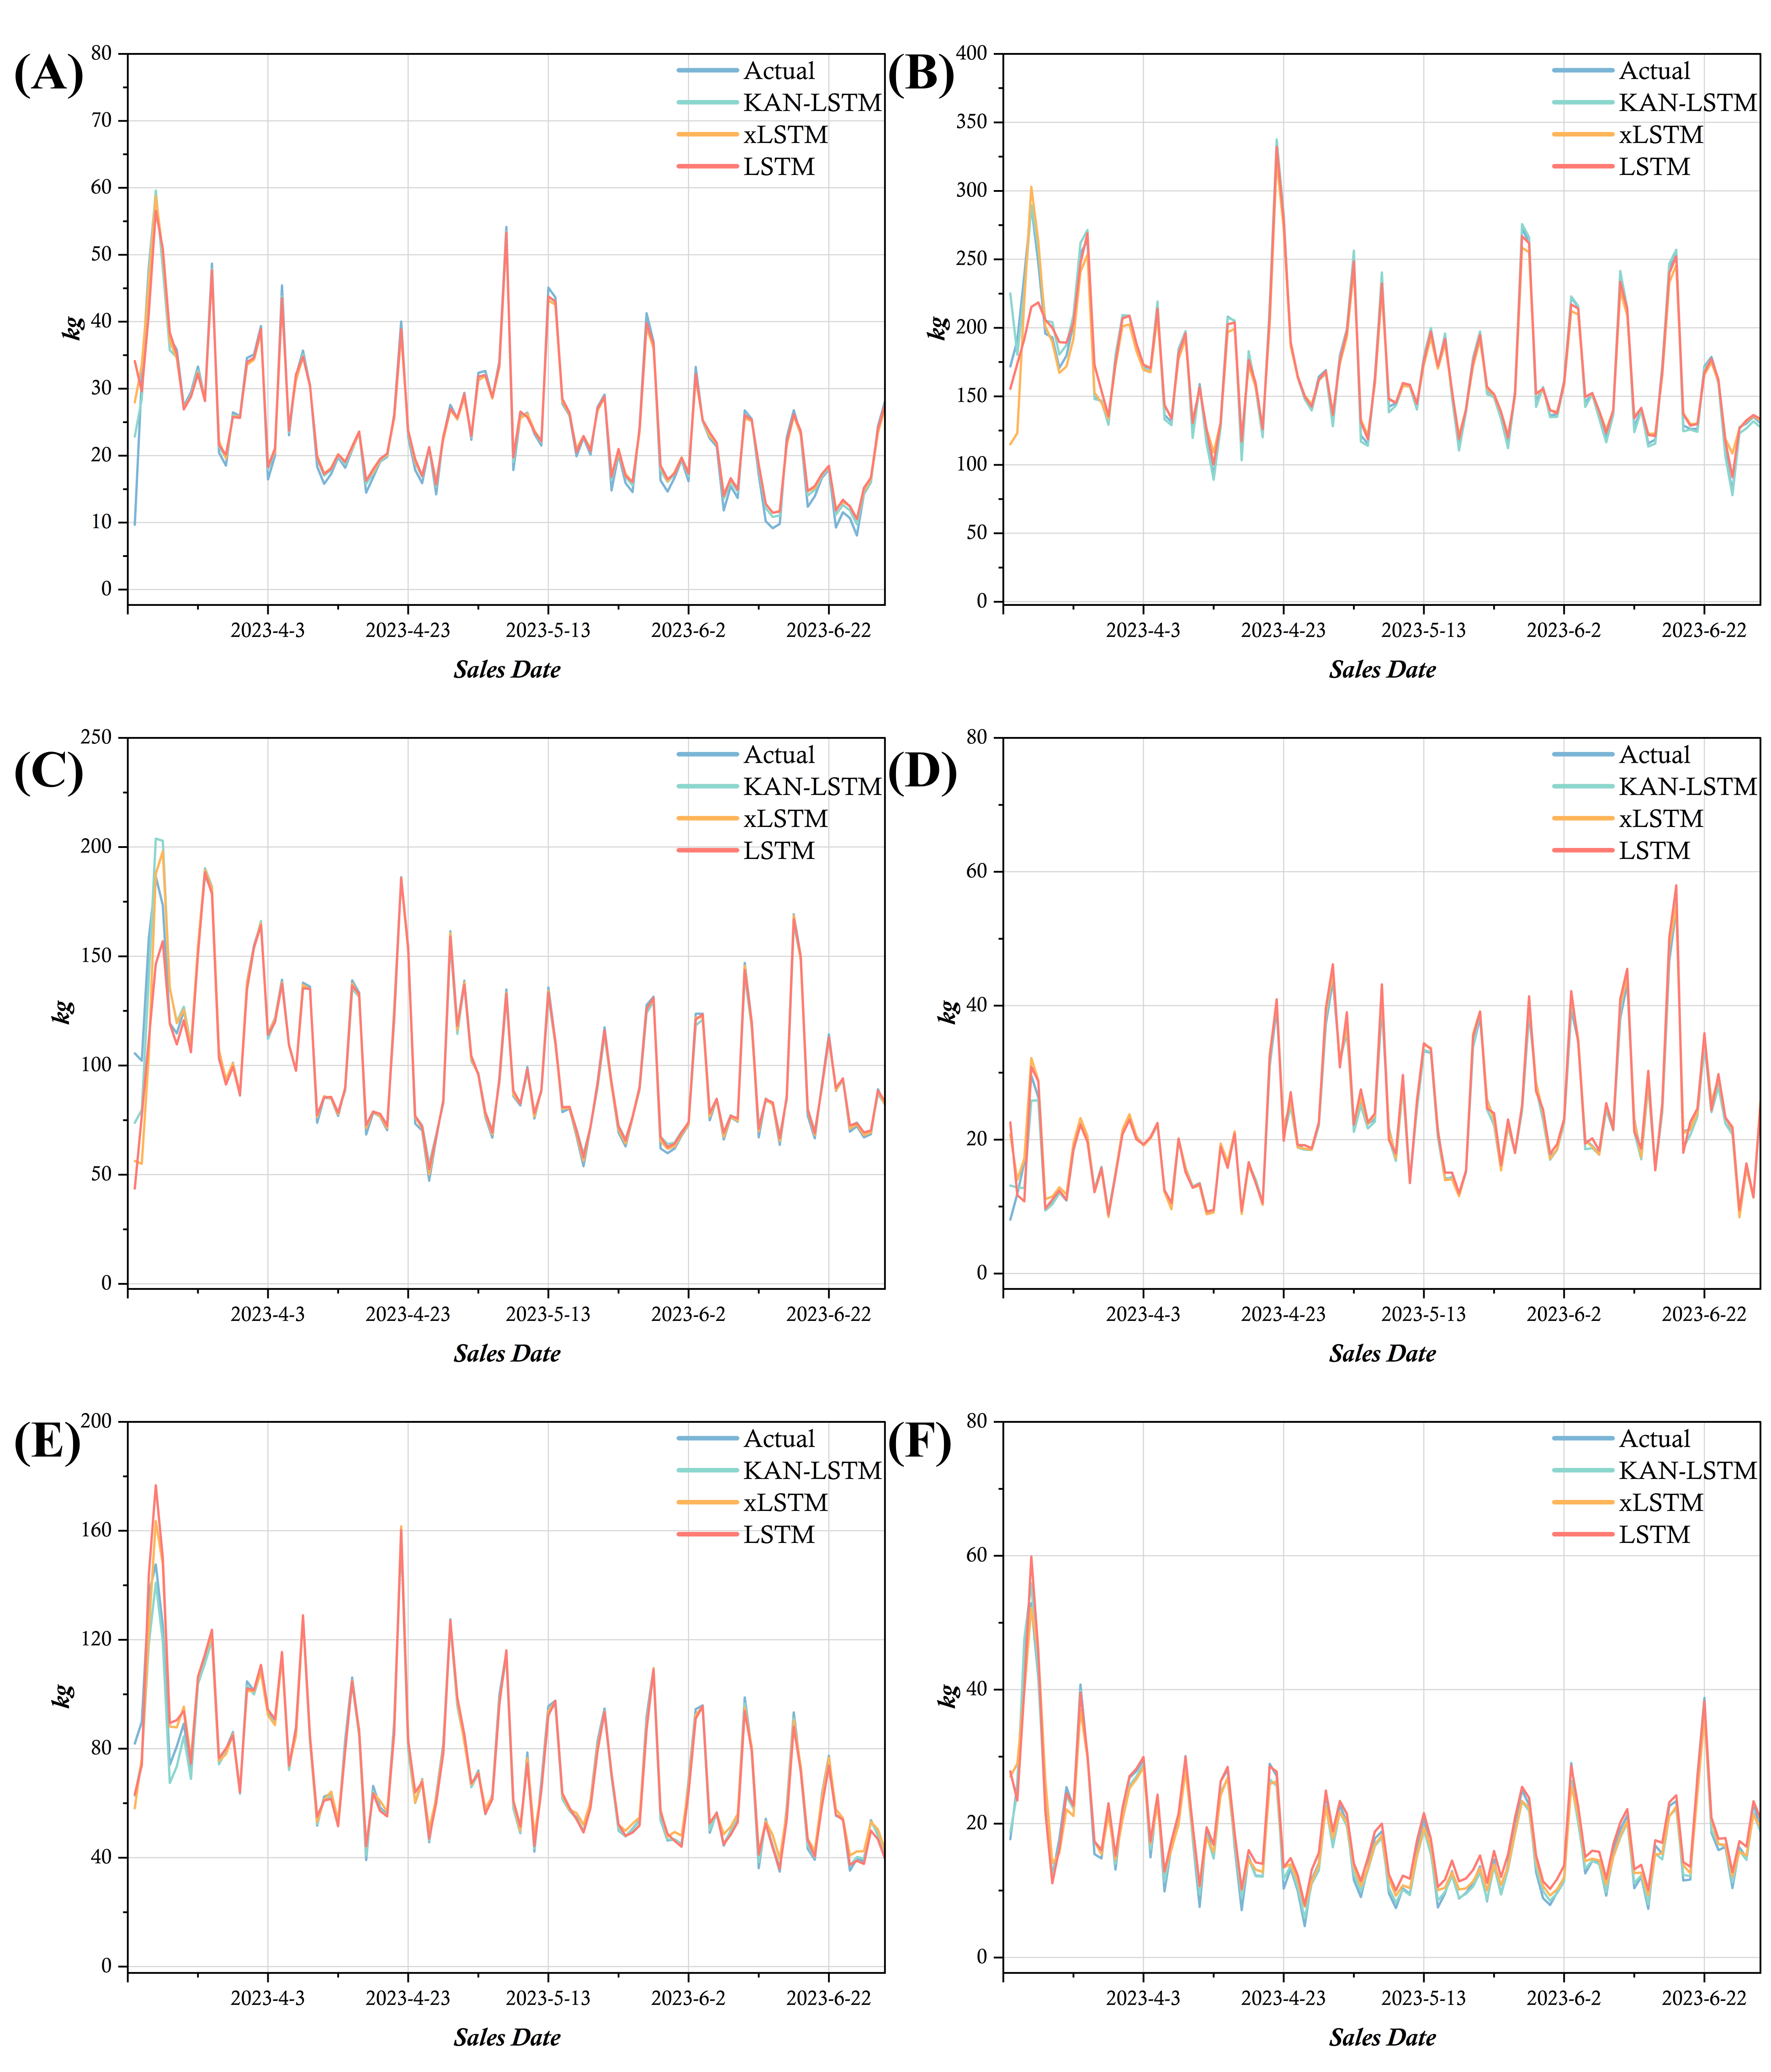
\includegraphics[width=1\textwidth]{图片12.png}
    \caption{365天窗口销量预测结果。(A)-(F)品类顺序同图\ref{fig:fig10}}
    \label{fig:fig12}
\end{figure}

\begin{figure}[H]
    \centering
    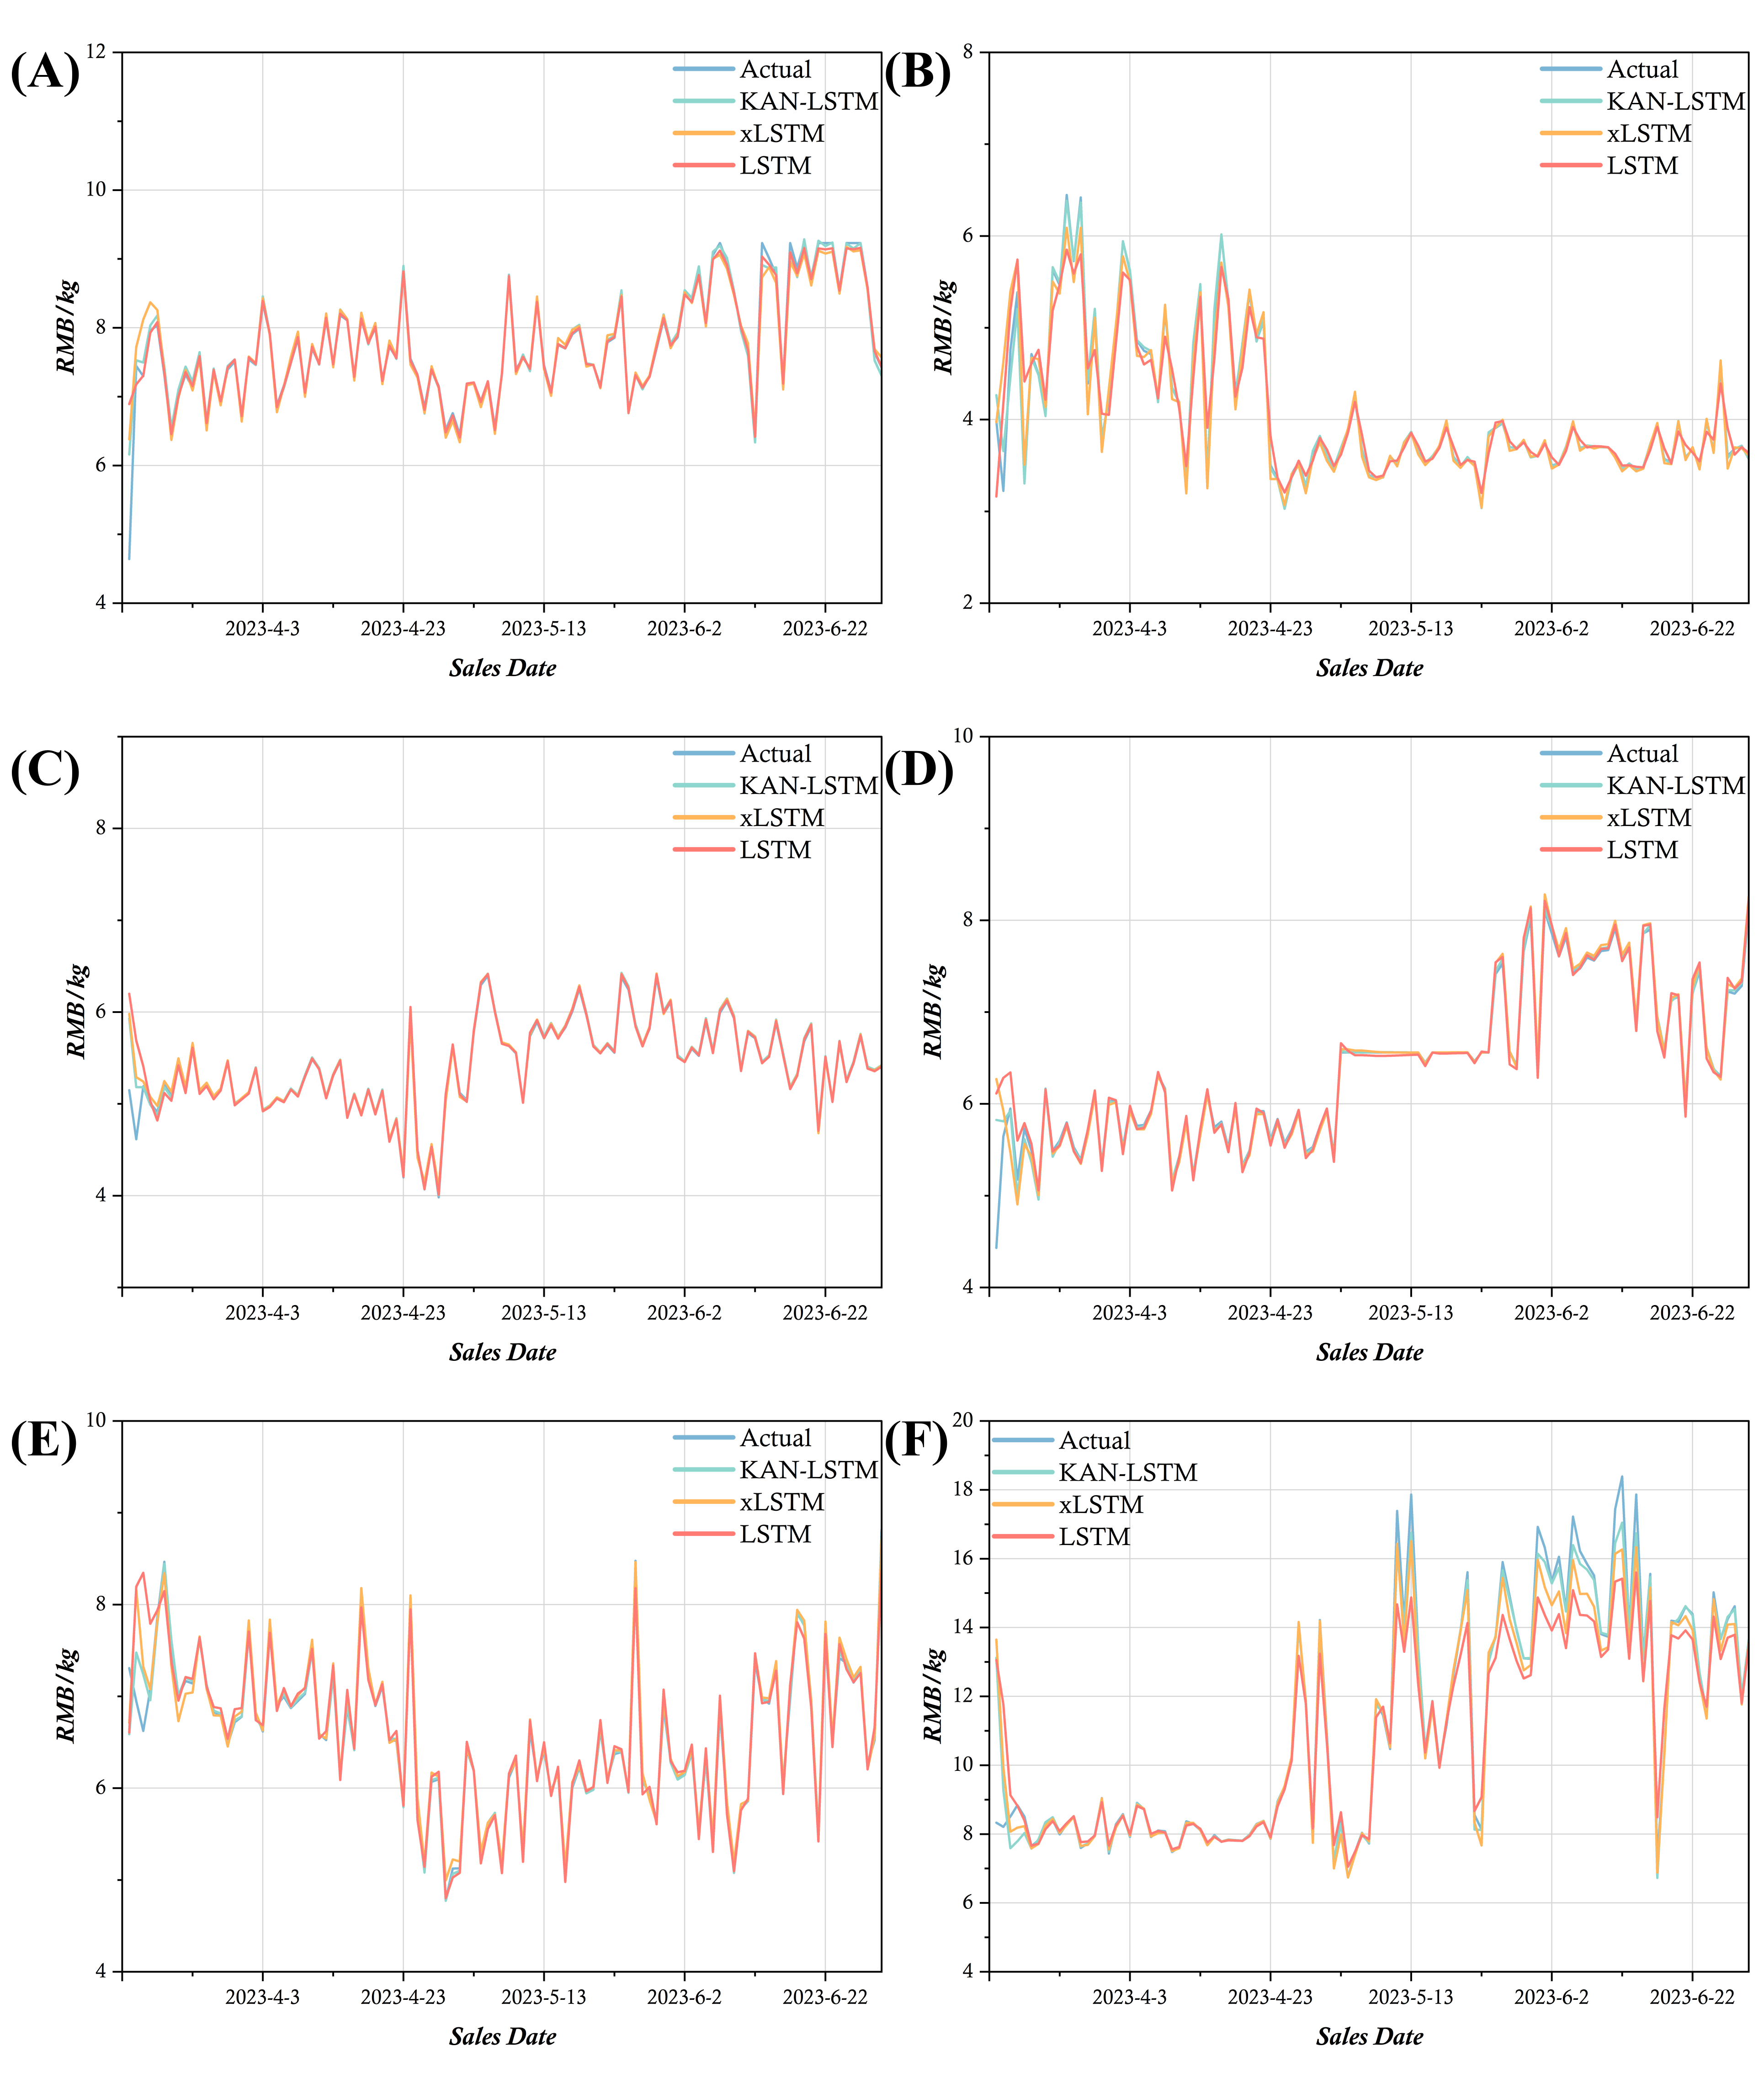
\includegraphics[width=1\textwidth]{图片13.png}
    \caption{365天窗口进货价格预测结果。(A)-(F)品类顺序同图\ref{fig:fig10}}
    \label{fig:fig13}
\end{figure}
\end{document}
